\newif\ifdraft
\drafttrue

\documentclass[12pt]{ucsddissertation}
% mathptmx is a Times Roman look-alike (don't use the times package)
% It isn't clear if Times is required. The OGS manual lists several
% "standard fonts" but never says they need to be used.

% Document class

\documentclass{IEEEtran}

\setlength{\paperheight}{11in}
\setlength{\paperwidth}{8.5in}
\usepackage[pass]{geometry}

% Packages 
%\usepackage{xcolor}
\usepackage{amsmath}
\usepackage{balance}
\usepackage[scaled=1]{inconsolata} % Use Inconsolata instead of CMTT
\usepackage{graphics}
\usepackage{graphicx}
\usepackage[hyphens]{url}%\urlstyle{tt}
\usepackage{listings}
\usepackage{multicol}
\usepackage{multirow}
\usepackage[scaled]{helvet}
\usepackage{rotating}
\usepackage{xspace}{}
\usepackage{algorithm}
\usepackage{comment}
%\usepackage{lmodern}
\usepackage[T1]{fontenc}
\usepackage{array}
\usepackage{tabu}
\usepackage[utf8]{inputenc}
\usepackage[table]{xcolor}
\usepackage{diagbox}
\usepackage{pifont}
\usepackage{xcolor}
\usepackage{booktabs}
\usepackage{relsize}
\usepackage{subcaption}
\usepackage{amsmath}
\usepackage[normalem]{ulem}

% Clickable link colors here:
\definecolor{linkcol}{rgb}{0,0,0}
\definecolor{citecol}{rgb}{0,0,0}
\definecolor{urlcol}{rgb}{0,0,0.75}

\newcommand\colname[1]{\emph{#1}}


%\usepackage{titlesec}
% Commands
%\newcommand{\todo}[1]{\ClassWarning{NOT READY TO SUBMIT}{There is something left todo} \textcolor{blue}{[TODO: #1 ]}}
\newcommand{\experiment}[1]{\textcolor{red}{Experiment: #1 }}
\newcommand{\highlight}[1]{\textcolor{red}{#1 }}
\newcommand{\goal}[1]{\textcolor{blue}{Goal: #1 }}
\newcommand{\transition}[1]{\textcolor{purple}{Transition: #1 }}
\newcommand{\blankfig}[0]{\framebox[3in]{\raisebox{0pt}[2in]{}}}

\ifdraft
\definecolor{notecolor}{rgb}{0.75,0,0} % A darker red
\definecolor{donecolor}{rgb}{0,0,1} % Blue
\newcommand{\note}[1]{{\textcolor{notecolor}{[\textit{#1}]}}}
\newcommand{\done}[1]{{\textcolor{donecolor}{[\textit{#1}]}}}
\usepackage{todonotes}
\else
\newcommand{\note}[1]{}
\newcommand{\done}[2]{}
\usepackage[disable]{todonotes}
\fi

\newcommand{\notefor}[2]{\note{\textbf{#1:} #2}}
\newcommand{\noteby}[2]{\note{#2 ---#1}}
\newcommand{\doneby}[2]{\done{#2 ---#1}}


\usepackage[bookmarks=true,%
	bookmarksnumbered=true,%
	colorlinks=true,%
	linkcolor=linkcol,%
	citecolor=citecol,%
	urlcolor=urlcol,%
	hypertexnames=true,%
	pdfpagelabels]{hyperref}

% Kirill's dainty list environments.

\newenvironment{prettylist}{
	\begin{list}{
		\footnotesize\raisebox{0.1mm}{\small\ding{118}}
	}{
		\setlength\topsep{2pt plus 1pt minus 1pt}
		\setlength\leftmargin{2em}
		\setlength\rightmargin{0pt}
		\setlength\itemsep{1pt plus.1pt}
		\setlength\parskip{0pt}
		\setlength\parsep{0pt}
		\setlength\itemindent{0pt}
	}
}{
	\end{list}
}

% Environments
\newenvironment{widelist}{\begin{list}{$\bullet$}{\setlength{\leftmargin}{.50cm}\setlength{\itemsep}{.1cm}}}{\end{list}}

\newcommand\bluetana{Bluetana}
\newcommand\iq{I/Q\xspace}


\makeatletter

\renewcommand\paragraph[1]{%
\@startsection{paragraph}{4}{\z@}%
{-0.75ex plus 0.05ex}{-0.5em}%
{\normalfont\normalsize\bfseries}{#1.}}

%\renewcommand\section{%
%\@startsection{section}{1}{\z@}%
%{-1.25ex plus -0.5ex minus -.2ex}%
%{0.75ex plus .25ex}%
%{\reset@font\large\bfseries}}
%
%\renewcommand\subsection{%
%\@startsection{subsection}{2}{\z@}%
%{-1.25ex\@plus -0.5ex \@minus -.2ex}%
%{0.5ex \@plus .2ex}%
%{\normalfont\large\bfseries}}
%
%\renewcommand\subsubsection{%
%\@startsection{subsubsection}{3}{\z@}%
%{-0.75ex\@plus -0.25ex \@minus -.25ex}%
%{0.25ex \@plus .2ex}%
%{\normalfont\normalsize\bfseries}}

\makeatother
\pagenumbering{gobble}

% Required information
\title{Mapping Short Range Wireless Links in Urban Infrastructure}
\author{Nishant Bhaskar}
\degree{Computer Science (Computer Engineering)}{Doctor of Philosophy}
% Each member of the committee should be listed as Professor Foo Bar.
% If Professor is not the correct title for one, then titles should be
% omitted entirely.
\chair{Professor Aaron Schulman}
% Your committee members (other than the chairs) must be in alphabetical order
\committee{Professor Patrick Pannuto}
\committee{Professor Stefan Savage}
\committee{Professor Geoffrey Voelker}
\committee{Professor Xinyu Zhang}
\degreeyear{2023}

% Start the document
\begin{document}
% Begin with frontmatter and so forth
\frontmatter
\maketitle
\makecopyright
\makesignature
% Optional
\begin{dedication}
    \setsinglespacing
    \raggedright % It would be better to use \RaggedRight from ragged2e
    \parindent0pt\parskip\baselineskip
    In of reading this manual before beginning to format the
    doctoral dissertation or master's thesis; for following the
    instructions written herein; for consulting with OGS Academic Affairs
    Advisers; and for not relying on other completed manuscripts, this
    manual is dedicated to all graduate students about to complete the
    doctoral dissertation or master's thesis.
    
    In recognition that this is my one chance to use whichever
    justification, spacing, writing style, text size, and/or textfont that
    I want to while still keeping my headings and margins consistent.
\end{dedication}
% Optional
\begin{epigraph}
    \vskip0pt plus.5fil
    \setsinglespacing
    {\flushright
    True ease in writing comes from art, not chance,\\
    As those move easiest who have learn'd to dance.\\
    'T is not enough to no harshness gives offence,---\\
    The sound must seem an echo to the sense.
    
    \vskip\baselineskip
    \textit{Alexander Pope}\par}
    \vfil
    \begin{center}
    You write with ease to show your breeding,\\
    But easy writing's curst hard reading.
    
    \vskip\baselineskip
    \textit{Richard Brinsley Sheridan}
    \end{center}
    \vfil
    \noindent Writing, at its best, is a lonely life. Organizations for
    writers palliate the writer's loneliness, but I doubt if they improve
    his writing. He grows in public stature as he sheds his loneliness and
    often his work deteriorates. For he does his work alone and if he is a
    good enough writer he must face eternity, or the lack of it, each day.
    
    \vskip\baselineskip
    \hskip0pt plus1fil\textit{Ernest Hemingway}\hskip0pt plus4fil\null
    
    \vfil
\end{epigraph}

% Next comes the table of contents, list of figures, list of tables,
% etc. If you have code listings, you can use \listoflistings (or
% \lstlistoflistings) to have it be produced here as well. Same with
% \listofalgorithms.
\tableofcontents
\listoffigures
\listoftables

% Preface
\begin{preface}
    Almost nothing is said in the manual about the preface. There is no
    indication about how it is to be typeset. Given that, one is forced to
    simply typeset it and hope it is accepted. It is, however, optional
    and may be omitted.
\end{preface}

% Your fancy acks here. Keep in mind you need to ack each paper you
% use. See the examples here. In addition, each chapter ack needs to
% be repeated at the end of the relevant chapter.
\begin{acknowledgements}
    I would like to acknowledge Professor Aaron Schulman  for his support as the
    chair of my committee. Through multiple drafts and many long nights,
    his guidance has proved to be invaluable. I would also like to thank my committee for their
    constructive feedback which helped me improve my thesis.

    Chapter 3, in full, is a reprint of the material as it appears in
    Please Pay Inside: Evaluating Bluetooth-based Detection of Gas Pump Skimmers. In USENIX Security Symposium (pp. 373-388).

    Chapter 4, in part, is a reprint of the material as it appears in 
    Evaluating Physical-layer BLE Location Tracking Attacks on Mobile Devices. In 2022 IEEE Symposium on Security and Privacy (SP) (pp. 1690-1704). IEEE.
    
\end{acknowledgements}

% Stupid vita goes next
\begin{vita}
    \noindent
    \begin{cv}{}
    \begin{cvlist}{}
    \item[2012] Bachelor of Engineering in Electronics and Instrumentation, \\
    Birla Institute of Technology and Science Pilani
    \item[2012--2015] Embedded Application Engineer, Texas Instruments Inc.
    \item[2015--2017] Teaching Assistant, Computer Science and Engineering\\University of California, San Diego
    \item[2017--2023] Research Assistant, University of California, San
    Diego
    \item[2019] Master of Science in Computer Science (Computer Engineering), \\
    University of California San Diego
    \item[2023] Doctor of Philosophy in Computer Science (Computer Engineering), \\
    University of California San Diego
    \end{cvlist}
    \end{cv}
    
    % This puts in the PUBLICATIONS header. Note that it appears inside
    % the vita environment. It is optional.
    \publications
    
    \noindent Nikoofard, A., Givehchian, H., Bhaskar, N., Schulman, A., Bharadia, D. and Mercier, P.P., 2022. Protecting Bluetooth User Privacy through Obfuscation of Carrier Frequency Offset. IEEE Transactions on Circuits and Systems II: Express Briefs.
    \\~\\
    \noindent Subbaraman, R., Bhaskar, N., Crow, S., Khazraee, M., Schulman, A. and Bharadia, D., 2022, June. Observing wideband RF Spectrum with low-cost, resource limited SDRs. In Proceedings of the 20th Annual International Conference on Mobile Systems, Applications and Services (pp. 617-618).
    \\~\\
    \noindent Givehchian, H., Bhaskar, N., Herrera, E.R., Soto, H.R.L., Dameff, C., Bharadia, D. and Schulman, A., 2022, May. Evaluating Physical-layer BLE Location Tracking Attacks on Mobile Devices. In 2022 IEEE Symposium on Security and Privacy (SP) (pp. 1690-1704). IEEE.
    \\~\\
    \noindent Jagtap, D., Bhaskar, N. and Pannuto, P., 2021, June. Century-scale Smart Infrastructure. In Proceedings of the Workshop on Hot Topics in Operating Systems (pp. 72-78).
    \\~\\
    \noindent Bhaskar, N., Bland, M., Levchenko, K. and Schulman, A., 2019, August. Please Pay Inside: Evaluating Bluetooth-based Detection of Gas Pump Skimmers. In USENIX Security Symposium (pp. 373-388).
    % This puts in the FIELDS OF STUDY. Also inside vita and also
    % optional.
\end{vita}

% Put your maximum 350 word abstract here.
%the !TEX root = paper.tex
\begin{abstract}

Gas pump skimming is one of the most pervasive forms of payment card attacks in
	the U.S. today.
%
Gas pump skimmers are easy to install and difficult to detect: criminals can open gas pump enclosures
	and hide a skimmer in internal payment wiring.
%
%Internal gas pump skimmers are also difficult to detect: they are not visible
%	from outside of the pump, and they blend into the wiring inside the pump.
%
As a result, officials have resorted to detecting skimmers by performing
	laborious manual inspections of the wiring inside gas pumps.
% 
In addition, criminals can also avoid being caught using skimmers: many gas
	pump skimmers have Bluetooth connectivity, allowing criminals to collect
	payment data safely from inside their car.
 
In this work, we evaluate if the use of Bluetooth in skimmers also creates an opportunity
	for officials to detect them without opening gas pumps.
%
%officials can scan detect skimmers by scanning for Bluetooth devices inside
	%gas pumps.
%
We performed a large-scale study where we collected Bluetooth scans at
	\visitedgasstations~gas stations in six states. We detected a total of
	\totalskimmers~Bluetooth-based skimmers across four U.S. states---all of which were
	recovered by law enforcement.
%
We discovered that these skimmers were clearly distinguishable from legitimate
	devices in Bluetooth scans at gas stations.
%
We also observed the nature of gas station skimming: skimmers can be installed
	for months without detection, and MAC addresses of skimmers may reveal the
	criminal entity installing or manufacturing them.
  
\end{abstract}


% This is where the main body of your dissertation goes!
\mainmatter

% Optional Introduction
\begin{dissertationintroduction}
    Big Picture

    Over the years, Bluetooth has become a popular short range communication technology in virtually everything - from personal devices (phone, smartwatch, tracker), payment systems, proximity detection systems, transportation (fleet trackers, car alarms) to industry and infrastructure (power grid, speed signs, traffic lights). These Bluetooth radios are fairly critical to not only our individual lives, but even to the proper functioning of our cities as a whole. 
    
    Improper or unauthorized use of any of these devices can have effects from the scale of individual safety to failure of financial and administrative institutions. Unfortunately, the deployment and maintainers of such electronic infrastructure make assumptions that they are aware of where and how such wireless radios are being used, and that Bluetooth technology protections will protect their privacy.
    
    In today’s world, Bluetooth sensors beacons are deployed in various urban places to enable proximity sensing, targeted ads and asset tracking and interaction with users. Further on, with the widespread use of social contact tracing, these systems have become even more important to ensuring spread of the pandemic
    
    In various kinds of infrastructure, Bluetooth modules that can be scanned for and connected to are being fitted as wireless implants. The aim is to allow maintainers and users easy access to internal buses for data and command exchange with the electronic systems, without needing to physically access the hardware. The maintainer simply needs to scan for the Bluetooth module and connect to it to run the necessary diagnostics. In transportation, Bluetooth modules are used with the internal OBD ports to allow easy vehicle diagnostics for applications such as vehicle repair and fleet tracking using a simple smart device. Further on, equipment such as traffic light controllers, speed signs are fitted with similar Bluetooth modules. On the power grid, equipment such as transformers, cap bank controllers etc which are located high up on poles are fitted with a Bluetooth radio for maintenance crews to diagnose issues and change settings without needing to climb the pole. All of these use cases show how Bluetooth devices have become integral to the smooth functioning of our urban areas.
    
    Unfortunately these electronic systems fitted with wireless radios work under the assumption of proper utilization of the radios, and inherent protections offered by Bluetooth technology. These assumptions don’t hold true, making them vulnerable to an attacker. Primarily, these devices are generally kept in discoverable or scannable mode, to make them visible and usable for legitimate users. This simple action makes them easily visible to any and all including the attacker.
    
    Bluetooth beacons rely on techniques such as MAC randomization to prevent unauthorized tracking, which has been proven to have several vulnerabilities. This can result in severe issues to user data privacy
    
    In case of infrastructure, these systems are typically deployed as install-and-forget, and since any person accessing such systems needs to be in close proximity the assumption is only legitimate users will attempt to access the system. This is thought to be a stronger guarantee especially since these systems are widespread, its hard to even know that such systems exist unless in proximity, and therefore need not be secured or monitored. To enable any maintenance personnel access to these systems, often they are left unsecured or use hardcoded passwords available in manuals online. This creates potential attack surfaces, even if one of which is exploited can cause huge problems, ex., one misconfigured traffic light controller at an intersection can cause massive accidents.
    
    In the most egregious cases, attackers can misuse lack of physical security and monitoring of infrastructure by installing their own implants to continuously exfiltrate data and often times misconfigure such infrastructure. A common and widespread example is criminals placing skimmers in gas pumps to steal payment card data of consumers. THis results in massive financial losses year on year to our financial institutions. The irony in this situation is that the same implicit assumption of invisibility unless in proximity is what criminals utilize knowing that no one will be able to find their device.
    
    Researchers in security understand the various problems associated with insecure Bluetooth radios. However, we don't have an insight into the scale of the problem in an urban setting. Particularly, what are the various Bluetooth devices that are being used, in what type of end equipment, and how they are being used. The fact that a number of such devices are visible to the world, can aid us in our search for these. Identification of the variety of Bluetooth devices in an urban setting can reveal potential attack surfaces, and is a necessary first step in securing our critical infrastructure.
    
    Challenges
    The task of identifying what Bluetooth devices are in deployment and attributing them to a defined end equipment is extremely challenging. We know that the devices we are hoping to observe are visible in Bluetooth scans, and so logic would dictate we just scan for them when in proximity. While  this approach sounds reasonable in theory, it’s extremely difficult to scale at urban levels. Such scans must be done in close proximity to devices due to the short range of Bluetooth radios. Wardriving based data collection of Bluetooth scans across the city is possible, but to cover all types of devices we need a lot of drivers.. Additionally, since wardrivers don’t stop to collect multiple scans around a piece of end-equipment (to begin with they don’t even know what to stop for), we end up getting very few scan records per device, if any.
    
    Even if such a wardriving exercise for Bluetooth scanning is performed, and a dataset is collected, identification is difficult because of limited information. Bluetooth scan responses (for classic Bluetooth) and advertisement scans (for Bluetooth LE) contain very little in terms of identifying information even for the radio. Bluetooth is intended as a short range peer to peer communication link, and therefore a user has no difficulty in identifying their Bluetooth device even with a simple name or MAC address. However, Bluetooth is so popular in all types of personal and commercial equipment, that any given location a simple scan leads to hundreds of different devices. Even if there are particular infrastructure in a small area that we are interested in, it still is a needle in a haystack problem. Further on, there is massive usage of popular Bluetooth radios, and particularly with implants, end-equipment manufacturers don’t bother changing the Bluetooth parameters to reflect information about the end-equipment. For example, during a wardriving exercise at a particular gas station,  I observed 4 radios with a very similar name. One was a speed sign, one was a fleet tracking system, one was a gas pump skimmer, and one was a traffic light controller.
    
    At the PHY layer, previous work indicates that by capturing the raw signals of WiFi radios, we can extract hardware impairment based information that is a unique identifier of the radio. We can use low cost SDRs to capture raw signals of the device discovery packets. Unfortunately, such techniques are hard to perform for Bluetooth radios. Bluetooth uses a narrowband GFSK modulation scheme with extremely short packets in device discovery. Measuring the hardware impairment based parameters with high resolution is extremely difficult. Furthermore, these parameters are known to be sensitive to the wireless environment and may not provide a unique enough identifier.
    
    Bluetooth devices can provide a list of services/UUIDs for devices that connect to them. A natural inclination is therefore to attempt connecting to some of these devices, especially ones that are unsecured or use default passwords. However, this is a wrong practice, especially when dealing with critical infrastructure in the field. We don’t have prior knowledge of command structure, and therefore we may inadvertently trigger an action that can lead to failure. In the case of illegal implants, connecting is even worse because we can overwrite critical forensic information that law enforcement uses to catch the criminals (e.x. last connected MAC address). Therefore, we have to restrict ourselves to simply the unconnected device discovery scan information for identification.
    
    In summary, to perform Bluetooth device identification at an urban scale we must rely solely on the limited information contained in device discovery packets collected through wardriving efforts, making it a challenging task.
    
    Thesis statement 
    In this dissertation, my goal is to design a generalized mechanism for identifying how Bluetooth devices are utilized in an urban environment. I will utilize information contained only in Bluetooth device discovery packets at both MAC and PHY layers, and combine it with geographic context information obtained from a data scanner. This information will be obtained from a combination of public and personally collected multi-year wardriving datasets. Within these constraints, I will show that even with a large number of Bluetooth devices in the environment,  it is possible to identify which devices correspond to urban infrastructure, and also that persistent PHY identification is possible even with MAC layer identifiers randomizing.
    
    My aim is to defend the following thesis statement: In the presence of a large number of Bluetooth devices at urban scale, we can utilize Bluetooth wardriving scans to 1) Identify particular equipment of urban infrastructure in which the legitimate devices are being used, 2) uniquely identify anomalous or illegitimate wireless devices in infrastructure, 3) Obtain persistent PHY layer identifiers that uniquely identify a wireless radio and are robust to changes in wireless environments
    
    
    Inventory or identification is a key first step in security audits for ensuring security of networked devices. Using this inventory, we can identify legitimate devices and the potential attack surfaces they expose, but also illegitimate devices interacting with our network. Such an identification is an important part of securing our organizational networks including critical infrastructure, and has been identified as an important initial step in various security frameworks like NIST, CISA (full names here)
    
    In recent times, a new class of connectivity solutions have emerged in urban infrastructure - Short range peer-to-peer devices. These devices, predominantly Bluetooth and WiFi modules, are attached to internal buses or available ports on infrastructure equipment. They provide easy, localized wireless access to maintainers for running diagnostics and configuring these infrastructure equipment. Authorized users simply scan for these wireless modules and connect to them using a smartphone/tablet, and are able to gain access to the functionality available.
    
    Current security audit methods are able to inventory network connected devices over any geographic scale, or unconnected devices within the confines of an organization building. Unfortunately, these short range peer-to-peer wireless links are at the intersection : they are not connected to a network, and are spread over entire metropolitan areas, and therefore have limited visibility with existing inventory approaches. This has resulted in several open attack surfaces for nefarious elements. Not only that, this limited visibility has encouraged criminals to attach their own such short range modules to infrastructure to gain unauthorized access (ex. gas pump skimmers)
    
    In this dissertation I tackle the problem of metropolitan scale identification of short range peer-to-peer wireless devices in infrastructure, by utilizing device discovery data collected from wardriving efforts. Using prior work, I show that it is possible to identify illegal wireless devices in fuel infrastructure using limited device discovery information, and that raw signal information can be utilized to extract persistent identifiers in large scale field settings. Finally, I propose a project to perform large scale inventory of such short range peer-to-peer wireless devices in urban infrastructure across multiple counties in the US. I discuss the technical and logistical challenges associated with such an effort, proposed ideas to tackle those challenges, and open research questions that I hope to answer.
    
\end{dissertationintroduction}

\chapter{Discovering illegitimate Bluetooth devices}
%!TEX root = paper.tex
%%% datadef.tex - Macros for various results used in tables and text.

\newcommand\pctmatchskimmer{3.98\%} % Percentage of classic bluetooth devices seen at gas stations that match the profile of skimmers

\newcommand\visitedgasstations{1,185} %Total number of gas stations visited in our study
%\newcommand\inspectedgasstationsAZ{757} %Total number of inspections by bluetana
\newcommand\inspectedgasstationsAZ{757} %Total number of gas stations visited in AZ in our study
\newcommand\visitedgasstationsAZ{491} %Total number of gas stations visited in AZ in our study
\newcommand\totaluncatstation{143} % Total number of gas stations where uncategorized BT devices were seen
\newcommand\visitedstationsMACCoDfiltered{79} % Number of gas stations visited where BT devices matching suspicious MAC + CoD were seen

\newcommand\totalskimmersBluetana{33}
\newcommand\Bluetanafraudprevented{\$495,000} % Total monetary fraud prevented by Bluetana assuming skimmers operated for one day. Will be the product of totalskimmersBluetana X 15,000

\newcommand\totalskimmers{64} %Total skimmers found in the field in our study
\newcommand\totalskimmersLE{23} %Total skimmers given to us by LE
\newcommand\totalskimmersseen{87} %Total skimmers ever detected by Bluetana. This is sum of found in field + obtained from LE
\newcommand\averageclassicBTperstation{2.2} %Average classic BT devices seen per gas station
\newcommand\stdevclassicBTperstation{2.05} % Std deviation of classic BT devices seen per gas station


%Following two macros are AZ specific and can be merged if we go through with AZ analysis
\newcommand\azskiminspect{7,325} %Total skimmer inspections done in Arizona 2016-2018.
\newcommand\azpercentskimfound{1.5\%} %Percentage of inspections Arizona 2016-2018 in which skimmers were found 
%%%%%%%%%%%%%%%%%%%


\newcommand\totalbtobserved{2,214} %Total number of BT devices observed across all visited gas stations
\newcommand\percentbtuncategorized{8.4\%} % Percent of total BT devices at visited gas stations that had uncategorized BT CoD
\newcommand\numberbtuncategorized{187} % Number of total BT devices at visited gas stations that had uncategorized BT CoD
\newcommand\numberBTMACCoDfiltered{102} % Number of total BT devices at visited gas stations that had suspect MAC + CoD
\newcommand\totalskimmersfirstvisit{42} % Total skimmers that were found in the visit to gas station (not including those found during a second visit to the gas station)


\newcommand\numvolunteers{44} %Total number of data collectors we had across US
\newcommand\skimmerfraudXVIIIUSA{\$17.43 million} % Total potential fraud in one day of operation of skimmers installed across SD,AZ,FL in 2018. Will be product of skimmers recovered X 15000

\newcommand\Bluetanaskimmerfield{33} %Skimmers found in the field without us 4 involved (Basically all of AZ, SDWM,LVPD)

\newcommand\Bluetanaskimstations{34} % Number of gas stations in which Bluetana saw a skimmer and it was recovered, US-wide

\newcommand\skimmeroneminutepercent{80\%} %Percent fraction of skimmers detected within one minute of arriving at a gas station

\newcommand\skimmerdetectiontimemedian{3} %Median time in seconds after entering 150 ft of gas station, when Bluetana can detect a skimmer 
\newcommand\skimmerdetectiontimemean{33} %mean time in seconds after entering 150 ft of gas station, when Bluetana can detect a skimmer 
\newcommand\skimmerdetectiontimestd{60} %mean time in seconds after entering 150 ft of gas station, when Bluetana can detect a skimmer 

%\newcommand\usssfyXVIIIincidents{13}
%\newcommand\usssfyXVIIIsksta{11}
%\newcommand\usssfyXVIIIstarisk{1.26\%}
%\newcommand\usssfyXVIIIrptsksta{2}
%\newcommand\usssfyXVIIIskimmers{42}
%\newcommand\usssfyXVIIIskperinc{3.2}
%
\newcommand\sdfyXVIIIskimmers{42}
\newcommand\azXVIskimmers{88}
\newcommand\azXVIIskimmers{57}
\newcommand\azXVIIIskimmers{148}
\newcommand\azALLskimmers{293}
\newcommand\flXVIskimmers{207}
\newcommand\flXVIIskimmers{650}
\newcommand\flXVIIIskimmers{972}
\newcommand\flALLskimmers{1,829}

\newcommand\sdfyXVIIIsksta{11}
\newcommand\azXVIsksta{54}
\newcommand\azXVIIsksta{46}
\newcommand\azXVIIIsksta{86}
\newcommand\azALLsksta{134}
\newcommand\flXVIsksta{162}
\newcommand\flXVIIsksta{432}
\newcommand\flXVIIIsksta{524}
\newcommand\flALLsksta{1,029}

\newcommand\sdfyXVIIIskperinc{3.2}
\newcommand\azXVIskperinc{1.6}
\newcommand\azXVIIskperinc{1.2}
\newcommand\azXVIIIskperinc{1.7}
\newcommand\azALLskperinc{2.2}
\newcommand\flXVIskperinc{1.3}
\newcommand\flXVIIskperinc{1.5}
\newcommand\flXVIIIskperinc{1.8}
\newcommand\flALLskperinc{1.7}

\newcommand\sdfyXVIIIskpercap{11.9} % 42 / (3.338m + 183k)
\newcommand\azXVIskpercap{4.3} % 88 / (20.66m)
\newcommand\azXVIIskpercap{2.7} % 57 / (20.98m)
\newcommand\azXVIIIskpercap{6.9} % 148 / (21.31m)
\newcommand\azALLskpercap{14.0} % 293 / (20.98m)
\newcommand\flXVIskpercap{10.0} % 207 /20.6m
\newcommand\flXVIIskpercap{31.1} % 650 / 20.9m
\newcommand\flXVIIIskpercap{45.6} % 972 / 21.3m
\newcommand\flALLskpercap{87.4} % 1829 / 20.93

\newcommand\fyXVIIIstart{October 1, 2017}
\newcommand\fyXVIIIend{September 30, 2018}

%\newcommand\azALLinspects{6,828}
%%\newcommand\azALLinspects{\smaller[3]\bfseries${}^{\texttt{{\textbackslash}azALL}}_{\texttt{\phantom{\textbackslash}inspects}}$}
%\newcommand\azXVIinspects{2,447}
%%\newcommand\azXVIinspects{\smaller[3]\bfseries${}^{\texttt{{\textbackslash}azXVI}}_{\texttt{\phantom{\textbackslash}inspects}}$}
%\newcommand\azXVIIinspects{1,857}
%%\newcommand\azXVIIinspects{\smaller[3]\bfseries${}^{\texttt{{\textbackslash}azXVII}}_{\texttt{\phantom{\textbackslash}inspects}}$}
%\newcommand\azXVIIIinspects{2,524}
%%\newcommand\azXVIIIinspects{\smaller[3]\bfseries${}^{\texttt{{\textbackslash}azXVIII}}_{\texttt{\phantom{\textbackslash}inspects}}$}
%
%\newcommand\azALLskinsp{2,894}
%%\newcommand\azALLskinsp{\smaller[3]\bfseries${}^{\texttt{{\textbackslash}azALL}}_{\texttt{\phantom{\textbackslash}skinsp}}$}
%\newcommand\azXVIskinsp{939}
%%\newcommand\azXVIskinsp{\smaller[3]\bfseries${}^{\texttt{{\textbackslash}azXVI}}_{\texttt{\phantom{\textbackslash}skinsp}}$}
%\newcommand\azXVIIskinsp{753}
%%\newcommand\azXVIIskinsp{\smaller[3]\bfseries${}^{\texttt{{\textbackslash}azXVII}}_{\texttt{\phantom{\textbackslash}skinsp}}$}
%\newcommand\azXVIIIskinsp{1,202}
%%\newcommand\azXVIIIskinsp{\smaller[3]\bfseries${}^{\texttt{{\textbackslash}azXVIII}}_{\texttt{\phantom{\textbackslash}skinsp}}$}
%
%\newcommand\azALLreginsp{3,934}
%%\newcommand\azALLreginsp{\smaller[3]\bfseries${}^{\texttt{{\textbackslash}azALL}}_{\texttt{\phantom{\textbackslash}reginsp}}$}
%\newcommand\azXVIreginsp{1,508}
%%\newcommand\azXVIreginsp{\smaller[3]\bfseries${}^{\texttt{{\textbackslash}azXVI}}_{\texttt{\phantom{\textbackslash}reginsp}}$}
%\newcommand\azXVIIreginsp{1,104}
%%\newcommand\azXVIIreginsp{\smaller[3]\bfseries${}^{\texttt{{\textbackslash}azXVII}}_{\texttt{\phantom{\textbackslash}reginsp}}$}
%\newcommand\azXVIIIreginsp{1,322}
%%\newcommand\azXVIIIreginsp{\smaller[3]\bfseries${}^{\texttt{{\textbackslash}azXVIII}}_{\texttt{\phantom{\textbackslash}reginsp}}$}
%
%\newcommand\azALLskinsppct{42.4\%} % 2894/6828
%%\newcommand\azALLskinsppct{\smaller[3]\bfseries${}^{\texttt{{\textbackslash}azALL}}_{\texttt{\phantom{\textbackslash}skinsppct}}$}
%\newcommand\azXVIskinsppct{49.4\%} % 939/2447
%%\newcommand\azXVIskinsppct{\smaller[3]\bfseries${}^{\texttt{{\textbackslash}azXVI}}_{\texttt{\phantom{\textbackslash}skinsppct}}$}
%%\newcommand\azXVIIskinsppct{}
%\newcommand\azXVIIskinsppct{40.4\%}
%%\newcommand\azXVIIIskinsppct{}
%\newcommand\azXVIIIskinsppct{36.9\%}
%
%%\newcommand\azALLreginsppct{}
%\newcommand\azALLreginsppct{57.6\%}
%%\newcommand\azXVIreginsppct{}
%\newcommand\azXVIreginsppct{50.6\%}
%%\newcommand\azXVIIreginsppct{}
%\newcommand\azXVIIreginsppct{59.6\%}
%%\newcommand\azXVIIIreginsppct{}
%\newcommand\azXVIIIreginsppct{63.1\%}
%
%%\newcommand\azALLincidents{}
%\newcommand\azALLincidents{232}
%%\newcommand\azXVIincidents{}
%\newcommand\azXVIincidents{61}
%%\newcommand\azXVIIincidents{}
%\newcommand\azXVIIincidents{54}
%%\newcommand\azXVIIIincidents{}
%\newcommand\azXVIIIincidents{117}
%
%%\newcommand\azALLskinc{}
%\newcommand\azALLskinc{7.3\%}
%%\newcommand\azXVIskinc{}
%\newcommand\azXVIskinc{3.3\%}
%%\newcommand\azXVIIskinc{}
%\newcommand\azXVIIskinc{5.5\%}
%%\newcommand\azXVIIIskinc{}
%\newcommand\azXVIIIskinc{10.2\%}
%
%%\newcommand\azALLreginc{}
%\newcommand\azALLreginc{92.7\%}
%%\newcommand\azXVIreginc{}
%\newcommand\azXVIreginc{96.7\%}
%%\newcommand\azXVIIreginc{}
%\newcommand\azXVIIreginc{94.5\%}
%%\newcommand\azXVIIIreginc{}
%\newcommand\azXVIIIreginc{89.8\%}
%
%%\newcommand\azALLinsphr{}
%\newcommand\azALLinsphr{8.0\%}
%%\newcommand\azXVIinsphr{}
%\newcommand\azXVIinsphr{5.1\%}
%%\newcommand\azXVIIinsphr{}
%\newcommand\azXVIIinsphr{7.2\%}
%%\newcommand\azXVIIIinsphr{}
%\newcommand\azXVIIIinsphr{12.5\%}
%
%%\newcommand\azALLskinsphr{}
%\newcommand\azALLskinsphr{6.1\%}
%%\newcommand\azXVIskinsphr{}
%\newcommand\azXVIskinsphr{2.6\%}
%%\newcommand\azXVIIskinsphr{}
%\newcommand\azXVIIskinsphr{3.9\%}
%%\newcommand\azXVIIIskinsphr{}
%\newcommand\azXVIIIskinsphr{9.1\%}
%
%%\newcommand\azALLreginsphr{}
%\newcommand\azALLreginsphr{8.2\%}
%%\newcommand\azXVIreginsphr{}
%\newcommand\azXVIreginsphr{5.2\%}
%%\newcommand\azXVIIreginsphr{}
%\newcommand\azXVIIreginsphr{7.6\%}
%%\newcommand\azXVIIIreginsphr{}
%\newcommand\azXVIIIreginsphr{13.1\%}
%
%\newcommand\azXVIadvantage{49.2\%}
%\newcommand\azXVIIadvantage{37.1\%}
%\newcommand\azXVIIIadvantage{17.9\%}
%\newcommand\azALLadvantage{30.6\%}
%
%\newcommand\azXVIencoreIII{6.5\%}
%\newcommand\azXVIIencoreIII{14.7\%}
%\newcommand\azXVIIIencoreIII{24.8\%}
%\newcommand\azALLencoreIII{17.6\%}
%
%\newcommand\azXVIencoreV{34.4\%}
%\newcommand\azXVIIencoreV{7.4\%}
%\newcommand\azXVIIIencoreV{51.3\%}
%\newcommand\azALLencoreV{36.6\%}
%
%\newcommand\azXVIvista{3.4\%}
%\newcommand\azXVIIvista{3.7\%}
%\newcommand\azXVIIIvista{2.6\%}
%\newcommand\azALLvista{3.1\%}
%
%\newcommand\azXVIovation{6.5\%}
%\newcommand\azXVIIovation{37.1\%}
%\newcommand\azXVIIIovation{3.4\%}
%\newcommand\azALLovation{12.1\%}
%
%%\newcommand\azALLsksta{}
%\newcommand\azALLsksta{172}
%%\newcommand\azXVIsksta{}
%\newcommand\azXVIsksta{54}
%%\newcommand\azXVIIsksta{}
%\newcommand\azXVIIsksta{42}
%%\newcommand\azXVIIIsksta{}
%\newcommand\azXVIIIsksta{76}
%
%%\newcommand\azALLstarisk{}
%\newcommand\azALLstarisk{8.7\%}
%%\newcommand\azXVIstarisk{}
%\newcommand\azXVIstarisk{2.8\%}
%%\newcommand\azXVIIstarisk{}
%\newcommand\azXVIIstarisk{2.1\%}
%%\newcommand\azXVIIIstarisk{}
%\newcommand\azXVIIIstarisk{3.8\%}
%
%%\newcommand\azALLskimmers{}
%\newcommand\azALLskimmers{299}
%%\newcommand\azXVIskimmers{}
%\newcommand\azXVIskimmers{85}
%%\newcommand\azXVIIskimmers{}
%\newcommand\azXVIIskimmers{63}
%%\newcommand\azXVIIIskimmers{}
%\newcommand\azXVIIIskimmers{151}
%
%%\newcommand\azALLstreet{}
%\newcommand\azALLstreet{\smaller[3]\bfseries${}^{\texttt{{\textbackslash}azALL}}_{\texttt{\phantom{\textbackslash}street}}$}
%%\newcommand\azXVIstreet{}
%\newcommand\azXVIstreet{\smaller[3]\bfseries${}^{\texttt{{\textbackslash}azXVI}}_{\texttt{\phantom{\textbackslash}street}}$}
%%\newcommand\azXVIIstreet{}
%\newcommand\azXVIIstreet{\smaller[3]\bfseries${}^{\texttt{{\textbackslash}azXVII}}_{\texttt{\phantom{\textbackslash}street}}$}
%%\newcommand\azXVIIIstreet{}
%\newcommand\azXVIIIstreet{\smaller[3]\bfseries${}^{\texttt{{\textbackslash}azXVIII}}_{\texttt{\phantom{\textbackslash}street}}$}
%
%%\newcommand\azALLstore{}
%\newcommand\azALLstore{\smaller[3]\bfseries${}^{\texttt{{\textbackslash}azALL}}_{\texttt{\phantom{\textbackslash}store}}$}
%%\newcommand\azXVIstore{}
%\newcommand\azXVIstore{\smaller[3]\bfseries${}^{\texttt{{\textbackslash}azXVI}}_{\texttt{\phantom{\textbackslash}store}}$}
%%\newcommand\azXVIIstore{}
%\newcommand\azXVIIstore{\smaller[3]\bfseries${}^{\texttt{{\textbackslash}azXVII}}_{\texttt{\phantom{\textbackslash}store}}$}
%%\newcommand\azXVIIIstore{}
%\newcommand\azXVIIIstore{\smaller[3]\bfseries${}^{\texttt{{\textbackslash}azXVIII}}_{\texttt{\phantom{\textbackslash}store}}$}
%
%%\newcommand\azALLskperinc{}
%\newcommand\azALLskperinc{1.3}
%%\newcommand\azXVIskperinc{}
%\newcommand\azXVIskperinc{1.4}
%%\newcommand\azXVIIskperinc{}
%\newcommand\azXVIIskperinc{1.2}
%%\newcommand\azXVIIIskperinc{}
%\newcommand\azXVIIIskperinc{1.3}
%
%%\newcommand\azALLskperskinc{}
%\newcommand\azALLskperskinc{1.5}
%%\newcommand\azXVIskperskinc{}
%\newcommand\azXVIskperskinc{2.5}
%%\newcommand\azXVIIskperskinc{}
%\newcommand\azXVIIskperskinc{1.3}
%%\newcommand\azXVIIIskperskinc{}
%\newcommand\azXVIIIskperskinc{1.5}
%
%%\newcommand\azALLskperreginc{}
%\newcommand\azALLskperreginc{1.2}
%%\newcommand\azXVIskperreginc{}
%\newcommand\azXVIskperreginc{1.3}
%%\newcommand\azXVIIskperreginc{}
%\newcommand\azXVIIskperreginc{1.2}
%%\newcommand\azXVIIIskperreginc{}
%\newcommand\azXVIIIskperreginc{1.3}
%
%
%%\newcommand\azALL{}
%%\newcommand\azXVI{}
%%\newcommand\azXVII{}
%%\newcommand\azXVIII{}
%
%
%%%% TABLE usss-results
%% Note: FY18 encoded using Roman numerals as fyXVII.
%
%\newcommand\usssfyXVIIIstart{October 1, 2017}
%\newcommand\usssfyXVIIIend{September 30, 2018}
%\newcommand\usssfyXVIIIincidents{13}
%\newcommand\usssfyXVIIIsksta{11}
%\newcommand\usssfyXVIIIstarisk{1.26\%}
%\newcommand\usssfyXVIIIrptsksta{2}
%\newcommand\usssfyXVIIIskimmers{42}
%\newcommand\usssfyXVIIIskperinc{3.2}
%
%%%% TABLE skimcost
%
%


%%the !TEX root = paper.tex
\begin{abstract}

Gas pump skimming is one of the most pervasive forms of payment card attacks in
	the U.S. today.
%
Gas pump skimmers are easy to install and difficult to detect: criminals can open gas pump enclosures
	and hide a skimmer in internal payment wiring.
%
%Internal gas pump skimmers are also difficult to detect: they are not visible
%	from outside of the pump, and they blend into the wiring inside the pump.
%
As a result, officials have resorted to detecting skimmers by performing
	laborious manual inspections of the wiring inside gas pumps.
% 
In addition, criminals can also avoid being caught using skimmers: many gas
	pump skimmers have Bluetooth connectivity, allowing criminals to collect
	payment data safely from inside their car.
 
In this work, we evaluate if the use of Bluetooth in skimmers also creates an opportunity
	for officials to detect them without opening gas pumps.
%
%officials can scan detect skimmers by scanning for Bluetooth devices inside
	%gas pumps.
%
We performed a large-scale study where we collected Bluetooth scans at
	\visitedgasstations~gas stations in six states. We detected a total of
	\totalskimmers~Bluetooth-based skimmers across four U.S. states---all of which were
	recovered by law enforcement.
%
We discovered that these skimmers were clearly distinguishable from legitimate
	devices in Bluetooth scans at gas stations.
%
We also observed the nature of gas station skimming: skimmers can be installed
	for months without detection, and MAC addresses of skimmers may reveal the
	criminal entity installing or manufacturing them.
  
\end{abstract}

%!TEX root = paper.tex
\section{Introduction}
\label{sec:intro}

% The story is can we augment slow and methodical with fast and maybe less good
% to save lots of money. Officers, NOT consumers.

% === Big picture picture ===
Payment card skimming attacks at gas pumps have reached alarming levels.
%
In 2018, law enforcement officials recovered 972 skimmers from gas pumps in Florida~\cite{florida-2018} and 148 skimmers from Arizona~\cite{arizona-2018} alone.
% 524 stations %at 11 stations %
Based on industry estimates, a single skimmer can capture 30--100 credit cards per day~\cite{rippleshot} and each card, based on estimates from law enforcement officials, nets the criminal an estimated \$500~\cite{ussc-guidelines}, resulting in a daily loss of \$15,000--50,000 per day of operation for each skimmer.\footnote{In Section~\ref{sec:background:money}, we compare these quoted estimates to other sources, and find them to be in agreement.} Less is known about how long a skimmer remains in operation, but allowing for even one day of operation per skimmer, 2018 losses exceed \$16 million across these two states.

Gas pumps are an ideal skimming target.
%
Gas pumps have relatively weak security: their payment circuitry can be accessed with universal keys or crowbars, and reading payment data is as easy as tapping into a ribbon cable (Section~\ref{sec:bkgd-skimhw}).
% 
Gas pump skimmers can be hidden inside of a gas pump enclosure, making them difficult to detect.
% 
As a result, inspectors have resorted to manually opening the pumps to inspect their wiring for skimmers.
%\footnote{These inspections are infrequently triggered by complaints.}
% 
Gas pump skimming has become so pervasive that the Arizona Department of Agriculture, Weights and Measures Division (AZWMSD) now checks for skimmers while doing routine inspections.\footnote{For example,
the ``Vapor Recovery Inspection Pre-Test Checklist'' has a checkbox for ``Checked for Skimmers''.}
%
From 2016 to 2018, the AZWMSD looked for skimmers in \azskiminspect~gas station inspections.
%
Inspectors found skimmers in only \azpercentskimfound~of these inspections.

Unfortunately, Law Enforcement (LE) rarely catch criminals while they are collecting payment data from gas pump skimmers.
%
The reason is, many gas pump skimmers are equipped with Bluetooth connectivity~\cite{krebs-siphoning,krebs-pos,krebs-gang,krebs-mexico}.
%
This allows criminals to remain in their car while wirelessly retrieving card payment data.
%
While Bluetooth is a vital tool for criminals to exfiltrate data from gas
pumps, it also could be an opportunity to make it easier to detect skimmers.

% === Our solution: Study Bluetooth ==== 

%that allow for operation from a safe distance
In this paper, we evaluate the effectiveness of detecting skimmers with 
Bluetooth scanning from a smartphone.
%
Indeed, if a skimmer can be detected with 
a smartphone, then authorities can discover and remove
skimmers passively and quickly while they visit a gas station for
other reasons.
% 
We built a smartphone application to perform this study, called Bluetana.
%
Bluetana collects all Bluetooth scan data that is available via
the Android Bluetooth APIs.
%---including information that has not been considered
%in the few Bluetooth skimmer detection tools that are available for consumers.
%
We equipped \numvolunteers~volunteers in six U.S. states with smartphones
running Bluetana. 
%
Our volunteers have collected scans at \visitedgasstations~gas stations, where
%
they observed a total of \totalbtobserved~Bluetooth devices.
%
In these scans, Bluetana detected a total of \totalskimmers~skimmers
installed at gas stations in Arizona, California, Nevada, and Maryland, and it
%
was the sole source of information
that led law enforcement to find \totalskimmersBluetana~skimmers.
%
%Assuming
%all of these skimmers were operating for at least one day, 
%we estimate that Bluetana prevented \Bluetanafraudprevented~in fraud.
%
%with Bluetana was the trigger for after we detected each skimmer we informed
%law enforcement, and they removed the skimmers and collected them as evidence.
%
%We estimate that the skimmers discovered by during this study stopped a
%total of \Bluetanafraudprevented~in fraud per day they were operating.

%
% They are also one of the largest owner-operated infrastructure that is slow to
% update to secure technology: there are $\sim$135,000 gas stations across the
% U.S., many of which still use magnetic stripe card readers and insecure PIN
% pads~\cite{emv2020}.
%
%This provides the key benefit of detecting skimmers before they have been used
%for enough fraud to trigger authorities to perform manual inspections (if it
%ever does).
%

%Bluetooth-based detection provides the additional benefit of revealing
%well-hidden skimmers.

% === Results ===

The primary result of this study is the first comprehensive look at how 
skimmers can appear in Bluetooth scans.
%
Namely, we observe that it is feasible to differentiate skimmers from other
common Bluetooth devices that appear in Bluetooth scans at gas stations (e.g.,
vehicle telemetry collectors).
%
The main differentiating factor for the skimmers we observed, is that the
Bluetooth Class-of-Device---a parameter not collected by any consumer Bluetooth
scanning applications that we are aware of---is ``Uncategorized''.
%for all of
%the skimmers we observed \noteby{JC}{for all of the skimmers}.
%
We also find that signal strength is a reliable way to determine if a Bluetooth
device is located near a gas pump, and thus could be a skimmer.
%
%even if it does not match the characteristics of typical skimmers.
%
%We also inadvertently ran a natural experiment where we observed the duration
%that skimmers can operate undetected in gas pumps: at least six months.

%(2) we observe that Bluetooth scanning is an effective tool for finding skimmers,

%for
%the Bluetooth signals from skimmers is today; and how effective it
%will be in the future.
 
Our study reveals several problems with consumer Bluetooth-based skimmer
detection applications~\cite{scaifeoakland,sparkfunapp,skimplus}:
%
(1) there are many legitimate products that appear at gas stations that use the
same Bluetooth modules as known skimmers; therefore, MAC address-prefix based detection 
may lead to false positives,
%
(2) there are many Bluetooth modules used in skimmers that do not comply with IEEE MAC
assignment requirements.
%
We also debunk advice on how to find skimmers with Bluetooth scans from authorities~\cite{ag-mn-skimmers} and viral information from social media~\cite{snopesskimmers}.
%
For instance, none of the skimmers we found using Bluetooth scans 
have a name that is a long string of letters and numbers.

Performing this in-depth study brought to light several important operational
lessons learned about the importance of detecting skimmers with Bluetooth.
%for
%improving skimmer inspections.
%
Using Bluetooth scans, officials detected skimmers while
driving by gas stations that they otherwise would not have inspected.
%
We also witnessed several instances where an inspector tried to find a skimmer,
but could not find it on their first pass looking inside a gas pump. However they persisted and found it based on the
knowledge that a suspected skimmer had appeared in
Bluetooth scans.
%
Surprisingly, we observed that there are skimmers installed in the same gas station, or
city, that have very similar MAC addresses---indicating their source is a
single criminal entity.
%
We even found skimmers installed hundreds of miles away that had surprisingly
close MAC addresses.

The rest of the paper is organized as follows: Section~2 provides background
on internal gas pump skimming: their construction, monetary incentive, and prevalence in
the wild. Section~3 is an overview of our large-scale Bluetooth scan collection methodology.
%for large-scale Bluetooth skimmer measurement study.
In Section~4, we
present the results of our study: what the skimmers we detected look like, how they compare to skimmers recovered independently by Law Enforcement, and
whether they are well hidden in the Bluetooth environment. In Section~5, we present
possible counter measures to the Bluetooth detection.  In Section~6 we present the operational lessons we
learned about skimming and criminal investigation procedure, while performing
our large scale measurement study. Section~7 is related work, and we conclude in
Section~8.

\if 0 % extra text {{{

Internal skimmers passively siphon track data, PIN keystrokes, and power, from
the PoS terminal's circuitry that sends all of this data in plain-text inside
the device (Section~\ref{sec:background:design}).

%
The primary advantage of Bluetooth-based detection is it can be crowdsourced:
authorities do not have to open PoS terminals to find skimmers, they can be
detected by anyone with a smartphone that is near a compromised PoS terminal.
%

We provide the first estimate of how much money criminals can make from
skimming (\todo{XXX} per skimmer) through a detailed analysis of carding
forums, combined with our own analysis of actual credit card data stored on
skimmers that were retrieved by law enforcement.
%


Also unlike ATMs, gas dispensers have been slow to update to new secure
technology because they are individually owned and operated\footnote{ATMs are
operated by a few large companies (i.e., Diebold and Cardtronics).}.

, and criminals delete the credit card numbers off of the skimmers as they
download them. 

The quintessential
skimmer is a a false face-plate overlay attached to an ATM's card slot that
records the card's track data, and a pinhole camera aimed at the PIN keypad to
record the PIN entry. 

ATM skimmers alone are estimated to cost over \$2 billion
globally~\cite{cnbc-skimmers}.

Upon finding a skimmer in a terminal during a manual inspection, they installed a
camera inside it to capture images of the criminal in the act of
retrieving the data~\cite{camera-in-pump}.

As evidence of this, the payment card industry has pushed back the deadline to
require gas stations to convert EMV chip payment technology to
2020, and it is likely to be pushed back again.



\fi %}}}

% Also that cellular skimmers are a thing http://newjersey.news12.com/story/38809657/consumer-alert-gas-station-gas-pump-credit-card-skimmers

% Also this is only going to get worse as the Bluetooth shimmer is now a thing https://www.sparkfun.com/sparkx/blog/2673

% "FICO, a credit scoring and analytics firm, noted that during the first half of 2017"

% https://www.muni.cz/en/research/publications/1073227
% https://www.muni.cz/en/research/publications/1362671
%
%European Financial Systems 2016, Proceedings of the 13th International Scientific Conference, year: 2016

%!TEX root = paper.tex
\section{Background}
\label{sec:background}

\begin{figure}
    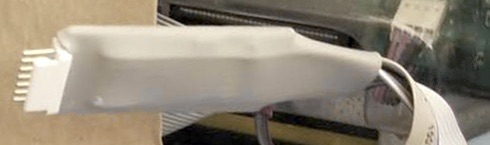
\includegraphics[width=0.95\linewidth]{skimmer/fig/wrapped-skimmer}
    \caption{An internal Bluetooth-based skimmer wrapped in grey tubing to blend in with the cabling inside the fuel pump. This skimmer
    was detected by \bluetana\ in Tempe, AZ.
%\noteby{NB}{Should we maybe put like a bigger picture with the entrails of the gas pump also visible?}}
}
\label{fig:wrapped-skimmer}
\end{figure}

\emph{Skimmers} are illicit devices that capture credit card magnetic stripe data when a card is used at a point-of-sale (PoS) terminal or automatic teller machine (ATM). External skimmers use a magnetic head concealed in a false
faceplate to read the magnetic stripe of a card as it is inserted into the real card reader. However, this paper is concerned
with a newer class of skimmers, called \emph{internal skimmers}, that are installed entirely inside a PoS
terminal or ATM, leaving no visual evidence of its presence~\cite{skimreaper2018}. Internal skimmers are attached inline to the cable that connects the
card reader to the main circuit board of the PoS terminal, tapping into the data and drawing power.
%
To make data collection easier, many internal skimmers include a Bluetooth-to-serial module that allows the
perpetrator to covertly collect the ``skimmed'' card data from a safe distance.
%
These skimmers are built using commodity hardware with a total unit cost of \$20 or less.

Fuel pumps
with a built-in PoS terminal have become a very popular target for such internal skimmers: they are unattended, easy
to access, and have poor physical security, which make it easy to install a skimmer without being noticed.
%
In a typical installation scenario, an attacker positions a van at a fuel station to block the station attendant's view of
the target pump (Excerpt in \ref{sec:appendix:cardsperskimmer}), opens the fuel pump using a common master key or crowbar, and clips a discreet gumstick-sized skimmer to the
ribbon cable between reader and main circuit board using a vampire clip (Figure~\ref{fig:wrapped-skimmer}). 
The entire process to install skimmer can
take less than 10 seconds~\cite{arizonareport}. The perpetrator can then return to the station with a 
smartphone, and without leaving their vehicle, connect to the skimmer using Bluetooth and download the card data.

\begin{figure}
    \centering
    \includegraphics[width=0.95\linewidth]{skimmer/fig/skimmer-example}
    \caption{Parts of a typical internal Bluetooth-based fuel pump skimmer. This skimmer
    was detected by \bluetana.}
    \label{fig:skimmer-example}
\end{figure}

\subsection{Internal Bluetooth Skimmers}
\label{sec:bkgd-skimhw}

The subject of our study are \emph{internal, Bluetooth-based skimmers} that are installed in fuel pump PoS
terminals. 
%
Figure~\ref{fig:skimmer-example} shows a typical Bluetooth skimmer, recovered from a fuel station in Southern California. This skimmer consists of a ``Teensy'' development board with an ARM Cortex-M4F
micro-controller and a Roving Networks \xspace{RN-42} Bluetooth-to-serial module. It also includes connectors 
for tapping into the wiring inside the pump (not shown). 

\paragraph{Connections} In the figure, the ribbon cable on the left intercepts or replaces the ribbon cable that connects the
magnetic stripe reader to the PoS terminal main board. The skimmer also uses this connection for power: the power and
ground pins of the Teensy (on far left of board, not visible in Figure~\ref{fig:skimmer-example}) are connected to
power and ground on the card reader cable. The ribbon cable on the right intercepts or replaces the ribbon cable from
the PoS keypad. This allows the perpetrator to capture additional card verification data, namely the debit card PIN
or credit card billing ZIP Code. Availability of a PIN code with a stolen debit card in particular, can increase its
value five-fold on the black market (Table \ref{tab:cardval}). However, not all skimmers capture keypad data.

Most gas station skimmers read the unencrypted data pulled from magnetic stripe readers.
%
Card issuers feel that removing sensitive data from the magnetic stripe on cards will help to solve
the problem~\cite{pcidss}.
%
Newer literature has demonstrated attacks on chip payment systems~\cite{bar2005known, bond2014chip}, and
law enforcement in Latin America have begun to find EMV skimmers that are Bluetooth enabled~\cite{krebshimmer,
customshimmer}.

\paragraph{Controller board} The skimmer pictured in Figure~\ref{fig:skimmer-example} used a Teensy micro-controller
development board equipped with a 120 MHz ARM Cortex-M4F micro-controller made by Freescale Semiconductor. By using a
development board, a skimmer requires only rudimentary electronic assembly: soldering wires to the development board.

However, skimmers have also been found using what appeared to be fully custom-designed boards. These are compact,
making them better for hiding in the dispenser. Examples of micro-controllers used in recovered skimmers include
Microchip PIC18F4550~\cite{sparkfunapp} and Atmel XMEGA128A4U~\cite{customshimmer}.

%\notefor{Nishant}{Please add additional examples of custom PCB skimmers from Web or skimmers we have seen ourselves; list \emph{exact} micro-controller and include a reference.}

%\noteby{NB}{Skimmers require minimal features on the micro-controller- low memory footprint[NB - Quote sparkfun website], two serial peripherals (to Bluetooth radio and mag reader), and a couple of GPIO/ADC(keypad) are all that are needed. In practice, skimmers recovered in the wild have been known to use various types of micro-controller boards.The first kind use readily available development boards, to enable fast prototyping. For example, the skimmer shown in figure uses a Teensy. In another kind of skimmers, criminals tend to simply re-purpose the micro-controller board on portable USB/Bluetooth mag readers, to use them as skimmers. The existing firmware can be used as is, but now to skim data. Finally, there are skimmers using custom boards based on a variety of micro-controllers (PIC18F, AtMega and others). While these boards take more effort to design and manufacture, the result is a compact skimmer which typically is hard to spot.}


\paragraph{Storage} The Teensy board also has a microSD card slot for additional data storage. Skimmers built on custom PCBs have also used flash and EEPROM ICs for storage. The storage capacities vary across designs, with examples using the PCT25VF032B (32-Mbit)~\cite{customshimmer} and M25P16VP (16-Mbit)~\cite{sparkfunapp}.

\paragraph{Bluetooth module} The skimmer shown in Figure~\ref{fig:skimmer-example} uses a Roving Networks RN-42 module, an inexpensive Bluetooth-to-serial module found in many skimmers. In Section~\ref{sec:bluetana:tool} we describe characteristics of popular Bluetooth-to-serial modules used in recovered skimmers for wireless data exfiltration. On the Bluetooth side, a Bluetooth-to-serial module provides a Serial Port Peripheral interface, which most operating systems recognize as a Bluetooth modem and instantiate a serial device for it. Operating systems will create a corresponding serial device, allowing user-space applications, namely a criminal's card dumping application, to communicate with the module. On the hardware side, a Bluetooth-to-serial module provides a TTL-level receive and transmit pin, allowing it to interface to any micro-controller UART. The module this allows even the simplest micro-controller to communicate via Bluetooth with a host device. The 2.4GHz Bluetooth antenna is included on the module's circuit board (exposed area to the left of the metal shield for the module shown in Figure~\ref{fig:skimmer-example}), so the antenna is also hidden.

Bluetooth-to-serial modules generally require no configuration, however, most
can be reconfigured using Hayes-style modem AT commands. In
Section~\ref{sec:bluetooth:skimmers} we describe the configuration capabilities
of popular modules. Notably, all of the Bluetooth-to-serial modules we found in
skimmers support changing the device MAC address, Bluetooth device name,
changing the pairing password, and the ability to become non-discoverable once
paired.

\subsection{Economics of Carding}
\label{sec:background:money}
Stealing and monetizing stolen credit and debit card data, called \emph{carding} by its practitioners, is a well-studied
form of financial fraud, however, reliable estimates of losses resulting from a single skimmer are difficult to find. To the criminal operating a skimmer, the expected revenue per skimmer breaks down as:
%
\[W = \textrm{(card value)}
\times \textrm{(cards per day)}
\times \textrm{(days deployed)}.\]
%\[W = \underbrace{\textrm{(card value)}}_{P}
%\times \underbrace{\textrm{(cards per day)}}_{Q}
%\times \underbrace{\textrm{(days deployed)}}_{D}.\]

Of these, we found published estimates for only the first two quantities, and very little about skimmer lifetimes. Here, we summarize the available data with the goal of estimating the losses incurred by a single skimmer.

\paragraph{Card value} To monetize stolen credit card data, skimmer installers have two options: sell the data on the black market, or cash out the cards on themselves. Based on our survey of sites selling stolen card data, black market prices for stolen cards fall in the \$10--220 range, depending on whether the card is a debit or credit card, and whether it comes with a PIN (for debit) or billing ZIP code (for credit). Table~\ref{tab:cardval} provides a summary of these prices with references. 

\begin{table}
\begin{tabular}{l@{\quad}lrl}
    \toprule
    \multicolumn{2}{l}{\colname{Scheme}} & \colname{Value} & \colname{Reference} \\
    \midrule
    \multicolumn{2}{l}{\textbf{Black market price}} \\
    & Debit, no PIN & \$20--30 & \cite{meccadumps,sellcvv,dumpsto, dumpsPrtShip} \\
    & Debit with PIN & \$110--220 & \cite{legitshop, sellcvv, dumpsPrtShip} \\
    & Credit, no ZIP & \$10--25 & \cite{meccadumps,sellcvv,dumpsto, dumpsPrtShip} \\
    & Credit with ZIP & \$25--60 & \cite{meccadumps,sellcvv,dumpsto, dumpsPrtShip} \\
    \multicolumn{2}{l}{\textbf{Cash-out value}} \\
    & Credit or Debit (standard) & \$400--800 & \cite{makingFirstMoney, cardingNewbieGuide, howToSucceedInStore, viceInterviewWithCarder} \\
    & Credit (premium) & \$1,000 & \cite{cardingNewbieGuide, santandWithdraw, honeyMoneyTut}\\
   \multicolumn{2}{l}{\textbf{Bank and merchant loss}} \\
%   & DOJ & \$902 & \cite{harrell2017} \\
%   & Arizona W\&M & \$1,003 & \cite{arizonareport} \\
    & Credit & \$1,003 & \cite{arizonareport} \\
%   & ATM Skimming & \$650 & \cite{ATMIA} \\
    & Debit & \$650 & \cite{ATMIA} \\
    \multicolumn{2}{l}{\textbf{Consumer liability}} \\
    & Debit (> 60 days) & unlimited & 15~USC~1693g \\ % \cite[\S1693g]{15uscode} \\
    & Debit (< 60 days) & max \$500 & 15~USC~1693g \\ % \cite[\S1693g]{15uscode} \\
    & Debit (< 2 days) & max \$50 & 15~USC~1693g \\ % \cite[\S1693g]{15uscode} \\
    & Credit & max \$50 & 15~USC~1643 \\ % \cite[\S1643]{15uscode} \\
     \multicolumn{2}{l}{\textbf{Prosecuted loss}} \\
%   & USSC & \$500 & \cite{ussc-guidelines} \\
    & Credit or debit & \$500 & \cite{ussc-guidelines} \\
     \multicolumn{2}{l}{\textbf{Court documents}} \\
     & Credit & \$362--400 & \cite{hristov,cristea,alisuretove,mekhakian} \\
     & Debit & \$665--1132 & \cite{estrada,aqel} \\

    \bottomrule
\end{tabular}

\caption{Value of stolen credit and debit cards.}
\label{tab:cardval}
\end{table}

Criminals can also cash out the cards themselves. Debit cards with a PIN are often cashed out by withdrawing money from an ATM, while credit cards are often cashed out by purchasing high-value merchandise (e.g. iPhones) and re-selling them. Reported cash-out values for debit and credit cards range between \$400 and \$1,000, depending on credit limit associated with the card.
%
We also conducted a survey of cash-out values reported in court documents involving skimmers.\footnote{We surveyed only documents available without fee from Court Listener.} Several cases reported specific cash-out values, rather than ranges. The debit card cash-out values were \$1132~\cite{hristov}, \$444~\cite{cristea} \$665~\cite{alisuretove}, \$1354~\cite{mekhakian}. The credit card cash-out values were \$362~\cite{aqel} and \$400~\cite{estrada}.

Losses due to credit and debit card fraud are borne largely by banks and merchants. This is likely because consumer liability for fraud in the U.S. is limited to \$50 for credit cards, and \$50 or more for debit cards (depending on how quickly the consumer reports the fraud).  Industry estimates for losses per-card incurred by banks are \$650 for debit cards and, \$1,003 for credit cards~\cite{arizonareport,ATMIA}. The U.S. Sentencing Commission estimates per-card losses at \$500 or more.

\paragraph{Cards per day} The number of cards a skimmer captures each day
depends on the number of transactions at that pump, which will vary by station.
Rippleshot, a payment fraud prevention service, states: ``a single compromised
pump can capture data from roughly 30--100 cards per day''~\cite{rippleshot}.
The lower end Rippleshot's estimate agrees with the estimate of 20--50 cards
per day we received from U.S. law enforcement agents. In addition, we found two
court documents that report criminals captured 25~\cite{estrada} and
30~\cite{alisuretove} cards per day.
%
We also studied 10 skimmers recovered from the field, which we were told were used and wiped daily. We found an average of 20 cards per skimmer, divided
evenly between debit and credit cards.\footnote{These skimmers were provided to
us because they were removed by the station owner, rather than LE, making them
unsuitable for use as evidence.}

\paragraph{Days deployed}  Internal skimmers are not limited by battery life
and can remain in operational indefinitely, because they draw power from the
PoS circuitry, Skimmer lifetime, then, is limited only by how long they can
remain undetected. Unfortunately, there is little reliable data on this. Our
only direct experience is our discovery of a pair of skimmers that remained
undetected for six months (Section~\ref{sec:blu:identify}). However, LE
informed us that criminals may leave skimmers in gas pumps after only a few days of retrieving 
card data and moving on to another location. Given the very limited data available on
skimmer lifetimes, we instead consider skimmer value \emph{per day of
operation}.

\paragraph{Cashout success rate}

Our analysis of court documents revealed that criminals are often unsuccessful
when trying to cashout a skimmed card. This may be due to a variety of reasons,
such as the following: incorrectly reading card data, hitting daily withdrawal
limits, and activating fraud alerts. Several cases mentioned that criminals
were not successful in cashing all skimmed cards. One case mentions a specific
cashout success rate of 47\%~\cite{mekhakian}.%, and the other was 50\%~\cite{rodriguez}.

\paragraph{Total skimmer value}

Finally, we estimate the range of per-day revenue from a skimmer based on the
prior figures. Our low end estimate is \$4,253 (25 cards per day, cashout of
\$362 per card, and 47\% cashout success rate), and our high end estimate is
\$63,638 (100 cards per day per day, \$1,354 cashout per card, and cashout success rate of
47\%).

\begin{comment}
Taking 30 cards per day, the lowest value in the Rippleshot range and near the middle of the estimate from law enforcement, and \$500 per card, the figure estimated by law enforcement officers and consistent with other estimates of cash-out value, places the value of each skimmer to the criminal at \textbf{\$15,000 per day}.

We compare this with a separate estimate obtained from information in court documents. Knowing that there is an equal distribution of credit and debit cards per skimmers, the average cashout value is at \$615 per card. With an average of 27 skimmer per card per day, and a lower bound success rate of 47.1\% in cashing out, the value of skimmer per day to the criminal stands at \$7820 per day.
\end{comment}

\begin{table}
\centering
\small
% Converted to vertical format by Aaron to manage space
\if 0
\begin{tabular}{lrrrrrrrrr}
\toprule
& \multicolumn{1}{c}{SD}
& \multicolumn{4}{c}{Arizona}
& \multicolumn{4}{c}{Florida}
\\
\cmidrule(lr){2-2}
\cmidrule(lr){3-6}
\cmidrule(lr){7-10}
%
\colname{Parameter}
& \colname{FY18}
& \colname{2016} & \colname{2017} & \colname{2018} & \colname{All}
& \colname{2016} & \colname{2017} & \colname{2018} & \colname{All}
\\
\midrule
Recovered skimmers
& \sdfyXVIIIskimmers
& \azXVIskimmers & \azXVIIskimmers & \azXVIIIskimmers & \azALLskimmers
& \flXVIskimmers & \flXVIIskimmers & \flXVIIIskimmers & \flALLskimmers
\\
Skimmed stations
& \sdfyXVIIIsksta
& \azXVIsksta & \azXVIIsksta & \azXVIIIsksta & \azALLsksta
& \flXVIsksta & \flXVIIsksta & \flXVIIIsksta & \flALLsksta
\\
Skimmers per incident
& \sdfyXVIIIskperinc
& \azXVIskperinc & \azXVIIskperinc & \azXVIIIskperinc & \azALLskperinc
& \flXVIskperinc & \flXVIIskperinc & \flXVIIIskperinc & \flALLskperinc
\\
Skimmers per million
& \sdfyXVIIIskpercap
& \azXVIskpercap & \azXVIIskpercap & \azXVIIIskpercap & \azALLskpercap
& \flXVIskpercap & \flXVIIskpercap & \flXVIIIskpercap & \flALLskpercap
\\
\bottomrule
\end{tabular}
\fi

\begin{tabular}{lcccc}
  \toprule
	\multicolumn{1}{p{1.5cm}}{\colname{Location \& Year}}          &
	\multicolumn{1}{p{2.0cm}}{\centering \colname{Recovered skimmers}}     & 
	\multicolumn{1}{p{1.5cm}}{\centering \colname{Skimmed stations}}       & 
	\multicolumn{1}{p{1.6cm}}{\centering \colname{Skimmers / \newline station}}     &
	\multicolumn{1}{p{1.8cm}}{\centering \colname{Skimmers / \newline $10^6$ people}}   \\
	\midrule
	\multicolumn{4}{l}{\textbf{San Diego}} & \\
	\hspace{0.4cm}FY 2018 & \sdfyXVIIIskimmers & \sdfyXVIIIsksta & \sdfyXVIIIskperinc & \sdfyXVIIIskpercap \\

  \multicolumn{4}{l}{\textbf{Arizona}} \\
	\hspace{0.4cm}2016 & \azXVIskimmers & \azXVIsksta & \azXVIskperinc & \azXVIskpercap \\
	\hspace{0.4cm}2017 & \azXVIIskimmers & \azXVIIsksta & \azXVIIskperinc & \azXVIIskpercap \\
	\hspace{0.4cm}2018 & \azXVIIIskimmers & \azXVIIIsksta & \azXVIIIskperinc & \azXVIIIskpercap \\
	\hspace{0.4cm}\textit{All}  & \azALLskimmers & \azALLsksta & \azALLskperinc & \azALLskpercap \\

  \multicolumn{4}{l}{\textbf{Florida}} \\
  \hspace{0.4cm}2016 & \flXVIskimmers & \flXVIsksta & \flXVIskperinc & \flXVIskpercap \\
	\hspace{0.4cm}2017 & \flXVIIskimmers & \flXVIIsksta & \flXVIIskperinc & \flXVIIskpercap \\
	\hspace{0.4cm}2018 & \flXVIIIskimmers & \flXVIIIsksta & \flXVIIIskperinc & \flXVIIIskpercap \\
	\hspace{0.4cm}\textit{All}  & \flALLskimmers & \flALLsksta & \flALLskperinc & \flALLskpercap \\

  \bottomrule
\end{tabular}

\caption{Prevalence of skimming in three regions of the U.S.}
\label{tab:wildskims}
\end{table}

\subsection{Skimmers Recovered in the Wild}
\label{sec:skimmersinwild}
To understand the prevalence of skimmers in the wild, we obtained data on recovered skimmers from three regions in the United States: San Diego and Imperial counties of California, with a combined population of 3.5 million; the state of Arizona, with a population of 7 million inhabitants; and the state of Florida, with a population of 21 million inhabitants. Table~\ref{tab:wildskims} summarizes the statistics. We note that these numbers do not represent \emph{all} recovered skimmers. For San Diego and Imperial counties, our statistics represent the number of skimmers found by or reported to a U.S. federal law enforcement agency. For Arizona and Florida, our statistics represent skimmers found by or reported to the AZWMSD and the Florida Department of Agriculture and Consumer Services.

The number of recovered skimmers has increased from 2016 to 2018 in both Florida and Arizona. The total number of skimmers recovered in 2018 across the three geographic regions is significant: if each skimmer operated for just one day, we estimate their total monetary impact would be ~\skimmerfraudXVIIIUSA. Yet, as the skimmers-per-million people number shows, the possibility of an average consumer encountering a skimmer at a gas station is quite small.

%%!TEX root = paper.tex
\subsection{Skimmers in the wild} %{{{
\label{sec:skimmersinwild}

\begin{table}
    \centering\small
    \begin{tabular}{lrrrr}
\toprule
\colname{Parameter} & \colname{2016} & \colname{2017} & \colname{2018} & \colname{All} \\
\midrule
\textbf{Routine Inspections} \\
\quad Total & 2,116 & 928 & 1,311 & 4,355 \\
\quad Found skimmers & 28 & 30 & 45 & 103 \\
\emph{Effectiveness} & 1.3\% & 3.2\% & 3.4\% & 2.4\% \\
\hline
\textbf{Complaint Inspections} \\
\quad Total & 53 & 63 & 128 & 244 \\
\quad Found skimmers & 3 & 5 & 12 & 20 \\
\emph{Effectiveness} & 5.7\% & 7.9\% & 9.3\% & 8.2\% \\

%Effectiveness of  & 2,116 & 928 & 1,311 & 4,355 \\
%Inspections triggered by Complaints & 53 & 63 & 128 & 244 \\
%Inspections recovering Skimmers & 28 & 27 & 38 & 93 \\
%Percent Skimmer Complaint Hits & 0 & 0 & 0 & 0 \\
%Percent Skimmer Investigation Hits & 0 & 0 & 0 & 0 \\
%(\%) Complaint-based Inspection Hits & \\
%\quad Avg. days since last insp. & 175.7 & 129.3 & 120.2 & 136.7 \\
%Skimmed stations & \azXVIsksta & \azXVIIsksta & \azXVIIIsksta & \azALLsksta \\
%\quad Gilbarco Advantage & \azXVIadvantage & \azXVIIadvantage & \azXVIIIadvantage & \azALLadvantage \\
%\quad Gilbarco Encore 300 & \azXVIencoreIII & \azXVIIencoreIII & \azXVIIIencoreIII & \azALLencoreIII \\
%\quad Gilbarco Encore 500s & \azXVIencoreV & \azXVIIencoreV & \azXVIIIencoreV & \azALLencoreV \\
%\quad Wayne Vista & \azXVIvista & \azXVIIvista & \azXVIIIvista & \azALLvista \\
%\quad Wayne Ovation & \azXVIovation & \azXVIIovation & \azXVIIIovation & \azALLovation \\
%Station risk  & \azXVIstarisk & \azXVIIstarisk & \azXVIIIstarisk & \azALLstarisk \\
%Skimmers recovered & \azXVIskimmers & \azXVIIskimmers & \azXVIIIskimmers & \azALLskimmers \\
%\quad Streetside & \azXVIstreet & \azXVIIstreet & \azXVIIIstreet & \azALLstreet \\
%\quad Storeside & \azXVIstore & \azXVIIstore & \azXVIIIstore & \azALLstore \\
%Sk. per incident & \azXVIskperinc & \azXVIIskperinc & \azXVIIIskperinc & \azALLskperinc \\
\bottomrule
\end{tabular}
    \caption{Routine inspections routinely do not find skimmers, but complaint-triggered inspections are significantly
    more likely to find skimmers.}
    \label{tab:azwm-results}
\end{table}

In previous subsections, we have identified the monetary cost of every single skimmer recovered in the field. In this subsection, we use data available from skimmer-hotbed areas of Arizona state and San Diego region to understand the prevalence of this problem. Armed with this understanding of gas station vulnerabilities in these regions that enable this problem, we perform a Google Street View based nationwide sampling of gas stations, to identify the potential prevalence of this threat across the US. Finally we close off by analyzing Arizona data further to understand effectiveness of current manual inspection methods and skimmer complaint mechanisms in Arizona. This motivates the need to augment existing investigative techniques with new pieces of information for improving the status quo.

\subsubsection*{Dataset Overview}

The Southwest of the U.S. is an area of elevated skimmer activity, leading us to focus on these two parts of the U.S.

The Arizona Department of Weights and Measures (AZWM) is tasked, among other responsibilities, with inspecting fuel dispensers for compliance with Arizona state laws and regulations. While the purpose of most inspections is not to search for skimmers, if inspectors do a find skimmers, they report this on the Fueling Device Inspection Form. AZWM makes all inspections reports available publicly in PDF form on their Web site.\footnote{\url{https://ctutools.azda.gov/PdfOriginals/}} The form includes the following data items: gas station street address, inspection date, time spent on the inspection, description of the complaint if inspection is based on a complaint, the last 5 inspections done at same location with date, and a description of the current inspection. If a skimmer is found, this is noted on the Fueling Device Inspection Form, and, in some cases, is accompanied by a Skimmer Inspection Form.

We downloaded all AZWM inspection reports and extracted all Fueling Device Inspection Form data and Skimmer Inspection Form data for analysis. Table~\ref{tab:azwm-results} summarizes our results.

\subsubsection{Prevalence of skimmers} %{{{

\paragraph{Arizona} \noteby{AS}{Nishant needs to write the rest of this text} \azALLskimmers~skimmers were
Recovered at skimmed stations, which amounts to \azALLskperinc~per incident.
While the number of skimmers are low, in section~\ref{subsec:skimcost} we show that the losses are huge

\paragraph{San Diego and Imperial counties} The San Diego office of the United States Secret Service is responsible
for San Diego and Imperial counties, which span the California--Mexico border. Unlike the AZWM, the USSS does not
routinely inspect fuel dispensers; all inspections are triggered by reports of a skimmer or a pattern of credit card
fraud that suggests a skimmer may be present at a fuel station.

%\begin{table}
%    \centering
%    \begin{tabular}{lr}
\toprule
\colname{Parameter} & \colname{FY18} \\
\midrule
% Inspections & XXX \\
Incidents & \usssfyXVIIIincidents \\
% Insp. hit rate & XXX \\
Sk. stations & \usssfyXVIIIsksta \\
Station risk & \usssfyXVIIIstarisk \\
Skimmers & \usssfyXVIIIskimmers \\
Sk. per incident & \usssfyXVIIIskperinc \\
\bottomrule
\end{tabular}
%    \caption{Summary of skimmer recovery statistics from the San Diego office of the United States Secret Service.}
%    \label{tab:usss-results}
%\end{table}

We obtained skimmer recovery statistics from the San Diego office of the United
States Secret Service for the 12 month period from October 1, 2017 to September
30, 2018. Table~\ref{tab:usss-results} summarizes these statistics.
\noteby{KL}{Discuss USSS results.}
\begin{comment}
\begin{figure}
    \centering
    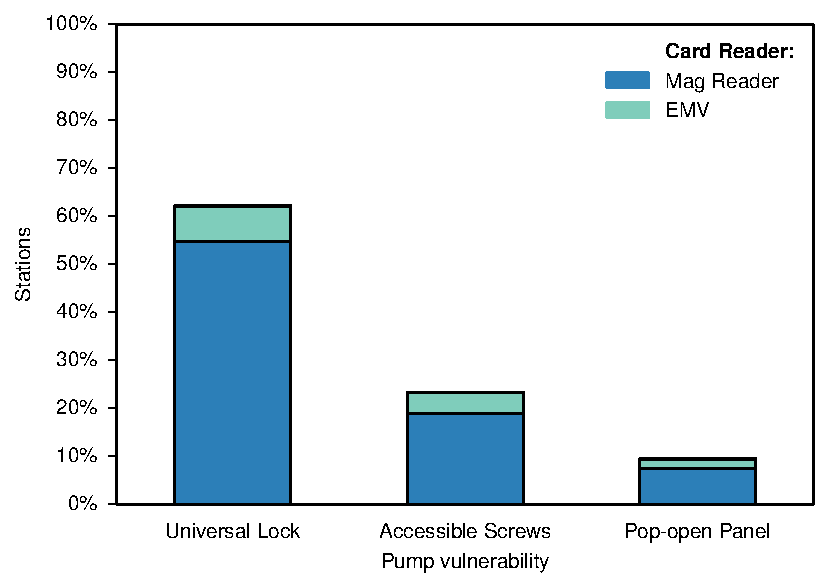
\includegraphics[width=\linewidth]{plots/barplot_us_vul_list.pdf}
    \caption{
    \label{fig:cdf_usvulgasstation}
    More than 80\% of gas stations across US, are still using easily accessible dispensers with magnetic card readers
    }
\end{figure}
\end{comment}
\paragraph{Nationwide prevalence of vulnerable pumps}
%

From the Arizona dataset we also know the make and model of gas dispensers on which skimmers were recovered. Gilbarco dispensers accounted for 84.8\% of skimmed stations with the numbers split between different models - Advantage (30.6\%), Encore 500s (36.6\%) and Encore 300 (17.6\%). Wayne dispensers accounted for 15.2\%. Since skimmers were discovered on these particular dispensers, a natural question arises - how common are these dispensers nationwide?

To answer this question, we performed a nationwide survey of gas stations across the US, with the aim of figuring out how prevalent are these particular dispensers. To identify the particular dispenser in service at a gas station, we can use Google Street View images, which surprisingly have a decent resolution for our task. We grouped all the gas stations across the US into population-served brackets using public FIPS data of the specific areas where the gas stations are located. The goal of population binning is to cover a wide variety of urban to semi-urban areas. In the top three population brackets - population in order of millions, order of hundreds of thousands and
order of tens of thousands, we randomly selected 0.5\% of all gas stations. For each of the gas stations selected, we manually inspected the Google Street View images to identify make and model of the dispenser. Additionally, since we know that there has been a push to retrofit these particular dispensers with EMV readers to remove the magnetic reader vulnerability, we identify the card reader with tha aim of understanding how widespread the use of EMV is. 

\begin{comment}
model and card reader type of dispensers. All the gas stations across the US
were divided into population-served brackets using public FIPS data of the
specific areas where the gas stations are located. In the top three population
brackets - population in order of millions, order of hundreds of thousands and
order of tens of thousands, we randomly selected 0.5\% of all gas stations, and
used Street View images to identify how many of these gas stations had
dispensers that suffered from three known vulnerabilites - use of a universal
lock, easily accessible door screws and pop-open card reader access.
Figure~\ref{fig:cdf_usvulgasstation} demonstrates the results.
\end{comment}
From the analysis, we observed that Gilbarco dispensers - Advantage, Encore 300 and Encore 500s are still the most popular across the country with 62.26\% of all dispensers sampled. Wayne Ovation and Vista account for another 32.79\%. The newer and secure models like Wayne Helix and Encore 700s currently only account for 1.61\% of all dispensers in the sample set, revealing the status quo of migration to secure dispensers. Even retrofitting to EMV had significantly low adoption. Of the 62.26\% of Gilbarco dispensers, only 7.44\% had EMV, and for Wayne this number stands at 6.43 \%. From these numbers, it can clearly be seen that the problem of skimmer vulnerable dispensers is significant all across the nation.

%}}}

\subsubsection{Effectiveness of inspections and complaints} %{{{

Analysis of Arizona inspection data reveals the challenges faced with the
status quo for skimmer discovery. While skimmer inspections comprised
\azALLskinsppct~of all inspections in the period from 2016-2018, skimmers were
recovered in only \azALLinsphr~of these. Skimmer complaints, often perceived to
be a viable source of skimming information, are surprisingly ineffective. Only
\azALLskinc~of successful skimmer inspections were due to a skimming complaint.
Worse still, of all the skimmer complaints only \azALLskinsphr~resulted in a
hit, revealing that these reports are also very unreliable. In this period,
skimmers were recovered at only \azALLsksta~gas stations, which meant that if
investigators were to randomly inspect an Arizona station, they only had a
\azALLstarisk chance of finding a skimmer. The year-by-year
breakdowns follow similar trends as the overall numbers. Interestingly though,
while the year 2018 saw a drop in ratio of skimmer
inspections~(\azXVIIIskinsppct)~over previous years, we observe a significant
increase in the number of incidents~(\azXVIIIincidents),~inspection hit
rate~(\azXVIIIinsphr)~and also number of skimmers
recovered~(\azXVIIIskimmers).~This is a result of increased knowledge among
consumers, station owners and the inspectors about skimmers. While this has
improved the effectivenss of skimmer inspections, still leaves a lot to be
desired.

\begin{figure}
    \centering
    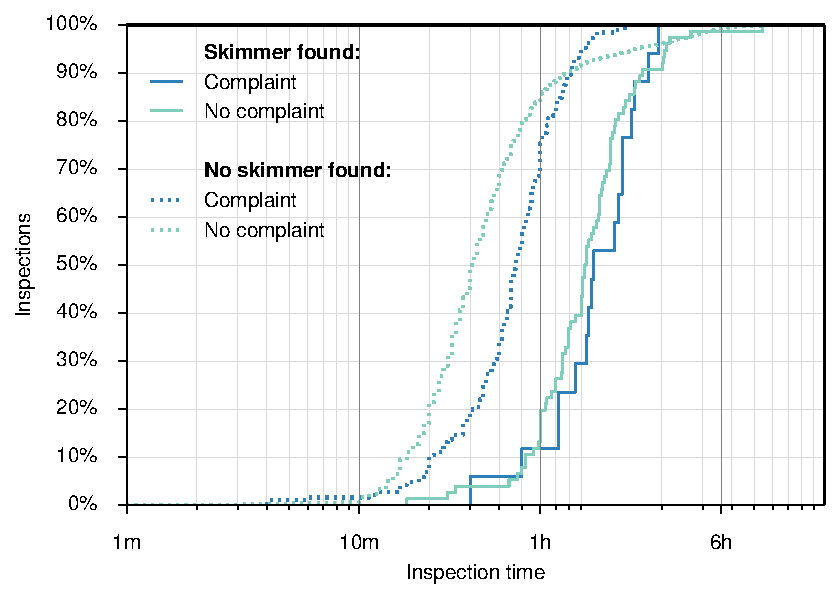
\includegraphics[width=\linewidth]{plots/arizona_analysis_all.pdf}
    \caption{
    \label{fig:cdf_arizona_timetaken}
    50\% of the unsuccessful manual inspections for skimmers took over half an hour to complete
    }
\end{figure}

But how costly in time is an inspection for Weights and Measures? All
inspection reports mention a start and end time for the inspection, and we use
that to analyze the time taken per inspection. Figure
\ref{fig:cdf_arizona_timetaken} shows the distribution of durations for
inspections that found skimmers and inspections that did not, split up by
whether inspection was triggered by a skimming complaint or not.

From the figure it can be observed that more time is spent in an inspection
when a skimmer was discovered. This is expected as the skimmer needs to be
carefully removed, tagged and bagged for forensic evidence. Also inspection
triggered by complaints take more time than their regular inspection
equivalents, which is also expected as a complaints need to be investigated
thoroughly. The interesting piece of information is the median time of
inspections. The median time for an unsuccessful inspection is 30 min (regular
inspection) and almost 50 min (complaint). From table~\ref{tab:azwm-results},
we know the number of unsuccessful inspections, and therefore the total time
spent by inspectors in unsuccessful inspections is 2,312 human-hours, or about
14 months(40 hours/week) of full time labor.Note that this is a conservative
estimate because it does not include transportation time, only the time spent
opening and searching fuel dispensers. Given limited agency resources, a
skimmer may be in place for months before it is found by a random inspection.
For 2018, we calculated the number of days to a successful skimmer recovery from a previous inspection at that same location and it turns out to be 120 days, which can result in significant monetary fraud.
%}}}

%}}}

%!TEX root = paper.tex


\section{Data Collection Methodology}
\label{sec:bluetana}

Driven by the observation that skimmers are hard to find---few pumps in San Diego, Arizona, and Florida have been found to have 
skimmers installed in them (Table~\ref{tab:wildskims})---we created a tool, called Bluetana, to evaluate the
effectiveness of Bluetooth-based skimmer detection.
%
We begin by presenting an overview of the tool and the data it collects.
%
Then we describe how Bluetana identifies suspicious devices and directs users
to collect additional data.
%
Finally, we discuss how we retroactively inspect data to find skimmers. 

\subsection{Crowdsourcing Bluetooth Scanning}
\label{sec:bluetana:tool}

We developed Bluetana, an Android-based measurement tool that officials and volunteers
use to scan for skimmers at gas stations.
%
%is an Android application that is provided to
%
Bluetana scans for nearby Bluetooth---both Classic and Bluetooth Low
Energy (BLE)---devices every 5~seconds using Android's Bluetooth API.
%
It collects the Bluetooth scans and geo-location data, and uploads this data to a
secure database over a cellular link.
%
Bluetana collects all of the Bluetooth scan data that Android makes available, including
Device name, MAC Address, Class-of-Device\footnote{Class-of-Device is twenty
  four bits indicating the device's intended use, such as \emph{smartphone} or
  \emph{speaker}.}, and signal strength (RSSI).

\paragraph{How we visited 1200 gas stations}
%
We outfitted ~\numvolunteers~ volunteers and inspectors in six U.S. states (CA, AZ, MD, NC,
NV, IL) with low-end smartphones running Bluetana in kiosk mode (they could not
close the application).
%
We selected officials who frequent gas stations as part of their daily job
duties. Primarily, they were Weights and Measures inspectors.
%Periodically, the application automatically transmits them over the cellular
%link to our secure database.
%
%It also records the device's geo-location during the scan when it completes. 

\subsubsection*{Indicating suspicious devices to inspire data collection}

\begin{figure}
\centering
\captionsetup{justification=centering}
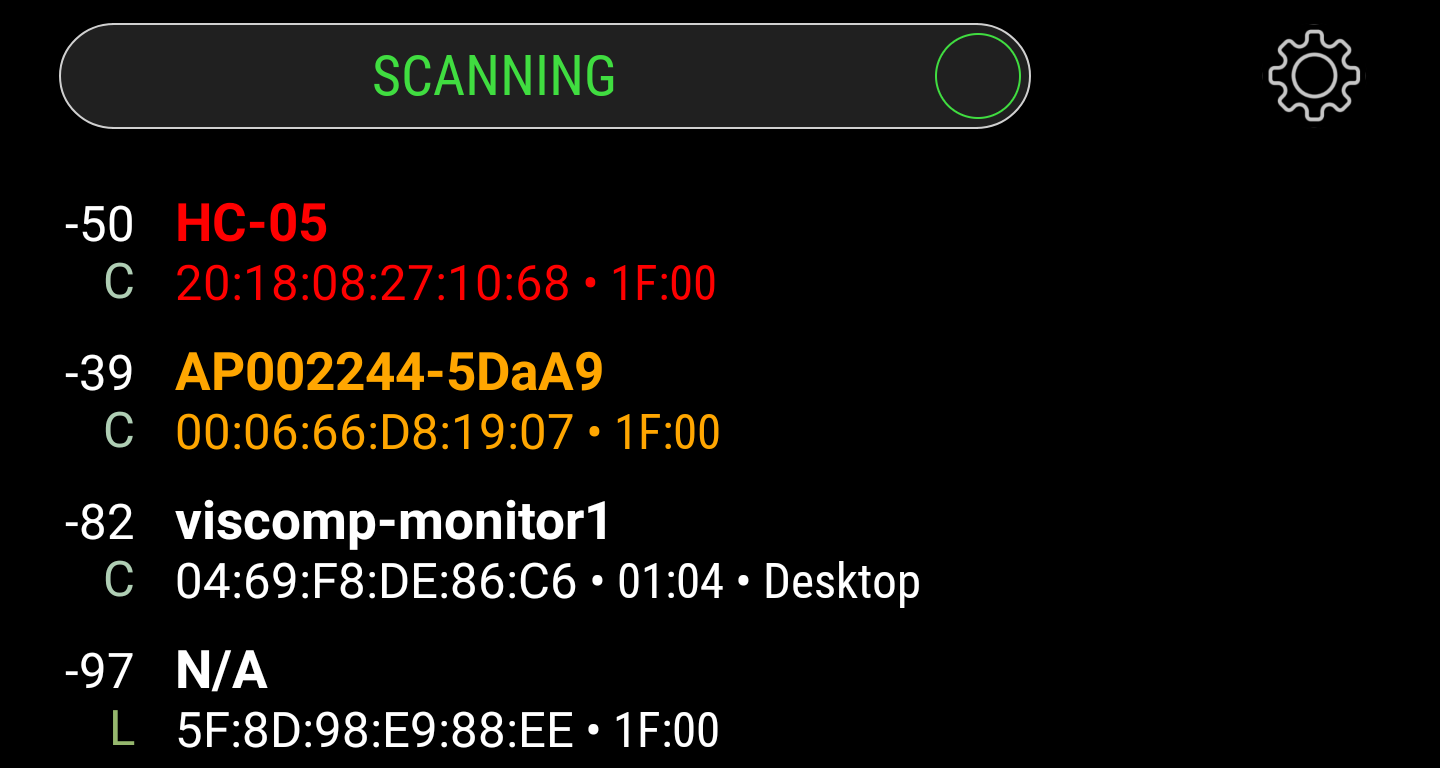
\includegraphics[width=0.8\linewidth]{skimmer/fig/bluetana_screenshot}
\caption{
\label{fig:bluetana}
The Bluetana user interface. Bluetana highlights suspicious devices, inspiring users to collect more
signal strength samples, and even perform inspections.
}
\end{figure}



The Bluetana display shows a list of Bluetooth devices detected during scanning.
%
When Bluetana detects a potential skimmer, it indicates this to the user by
highlighting the device record (Figure~\ref{fig:bluetana}).
%
The Bluetooth scan profile of the modules that have been found in skimmers inform which devices we highlight in Bluetana.
 
Skimmers recovered by LE are often found to use CSR (Qualcomm) chip-set-based Bluetooth modules.
%, and criminals
%tend to leave the Bluetooth properties of these modules at their factory defaults.
%
Our highlighting procedure primarily looks for the default Bluetooth profile of
these modules---with the exception of the Device Name which can be missing due to poor
signal strength, and modified by criminals in an attempt to hide the device (Section~\ref{sec:bluetooth}).
%
The factory default Bluetooth scan profile (i.e., MAC prefix, Device Name, and
Class-of-Device) of these modules are as follows:

\begin{center}
    \begin{tabular}{r|c|c|c}
        \textbf{Mod.} & \textbf{MAC Prefix} & \textbf{Dev. Name} & \textbf{Class of Dev.} \\ 
        \hline RN & \texttt{00:06:66} & ``\texttt{RBNT-*}'' & Uncategorized
				\\ HC & \textit{Various} & ``\texttt{HC-05/06}'' & Uncategorized \\
    \end{tabular}
\end{center}


%In our study, we detect many skimmers have Bluetooth modules configured with the default scanning profile.
%
%However, in our study we also observe that criminals have been found to modify the Device Name .
%
%Therefore, we include exceptions for 



Bluetana chooses a highlight color via a three-step decision process, depicted in Figure~\ref{fig:bluetana-flagging-flow}.
%
First, the app checks the device's class.
%
All skimmers studied within this work, whether discovered by Bluetana or not, had a device class of \emph{Uncategorized}.
%
If the device class is not uncategorized, the data is saved for later analysis.
%
The device's MAC prefix is then compared against a ``hitlist'' of prefixes used in skimming devices recovered by law enforcement.
%
If the device has a MAC that is not on this hitlist, it is unlikely to be a skimmer, and the app highlights the record yellow.
%
Next, if the device name matches a common product using the same MAC prefix, the record highlights in orange.
%
If all three fields (MAC prefix, Class-of-Device, and Device Name) indicate the device is likely to be a skimmer, Bluetana highlights the record in red.
%
The highlighting procedure is the result of a year of refinements based on our experience finding skimmers in the field, and Bluetana includes a remote update procedure to account for these incremental changes.

\begin{figure}[!h]
  \centering
  \captionsetup{justification=centering}
  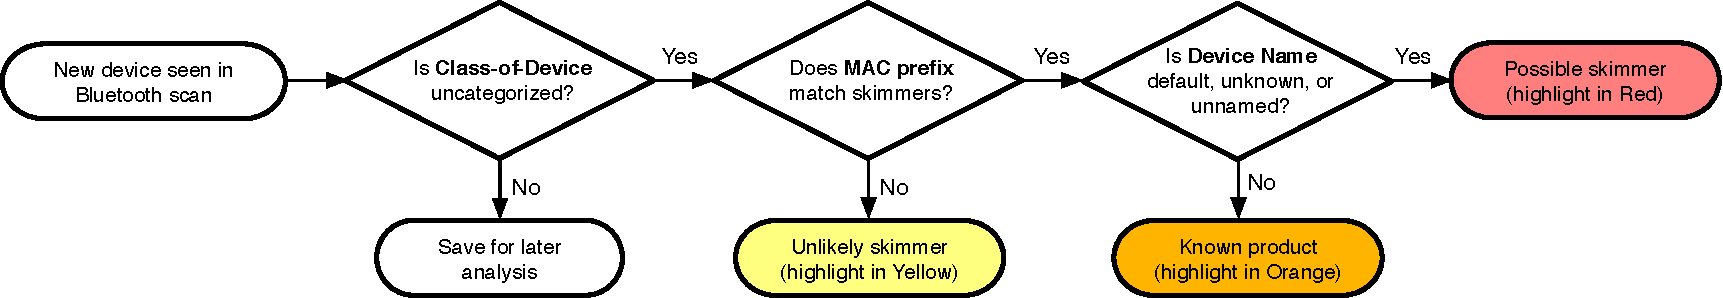
\includegraphics[width=\linewidth]{skimmer/fig/bluetana-flagging-flow}
  \caption{
  The procedure Bluetana uses for highlighting suspicious devices.
  %The MAC address of the device is first checked against a
  %hitlist of known skimming devices. Is this check succeeds, the Class-of-Device and
  %device name of the device are checked for innocuity. If these checks fail, the device
  %is flagged as a potential skimmer.
  \label{fig:bluetana-flagging-flow}
  }
  \end{figure}
  

This simple highlighting proved to be vital to our data collection.
%
Red serves as a cue to perform signal strength localization:
%
it directed our users to collect more samples of signal strength to determine
if a device is located in the gas pump area---and is therefore likely to
be a skimmer. 
%
In several cases, Bluetana highlighting a device in red was the only reason officials performed a manual skimmer inspections:
%
out of the \totalskimmers~skimmers we found, \Bluetanaskimmerfield~were recovered
because an official started an inspection only after noticing a device was highlighted in red in Bluetana.
%

In one instance, an Arizona Weights and Measures inspector was driving by a gas station when two red highlighted devices appeared in Bluetana.
%
He made an unscheduled stop at the gas station, performed a skimmer inspection, and discovered two skimmers.
%
Figure~\ref{fig:arizona_driveby} shows a portion of the official Arizona inspection report documenting this incident.

\begin{figure}[!h]
  \centering
  \captionsetup{justification=centering}
  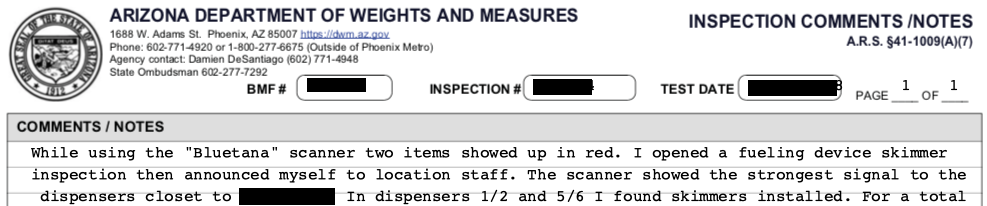
\includegraphics[width=\textwidth,height=3cm]{skimmer/fig/arizona_driveby_anecdote.png}
  \caption{
  \label{fig:arizona_driveby}
 Bluetooth scanning helps inspectors find more skimmers because they detect skimmers when driving by a gas station.
  }
\end{figure}

Bluetana's highlighting procedure is more comprehensive than other skimmer detection apps on the Play Store.
%
Scaife et al. \cite{scaifeoakland} investigated the behavior of these apps and found that they flag skimmers based on either MAC prefix or Device Name.
%
These apps would miss skimmers with non-standard MAC prefixes or customized (missing) device names which Bluetana was able to find (Section~\ref{sec:bluetooth:skimmers}).
%
Bluetana also found legitimate devices that would be considered skimmers by these apps (Section~\ref{sec:bluetooth:scans}).

\begin{comment}  
As a result, the application accounts for the entire Bluetooth scan
response and is more comprehensive than any Bluetooth skimmer scanning
application available.
%
A rigorous study of Bluetooth-enabled skimmer detection applications was performed by Scaife et al.
\cite{scaifeoakland} and found majority of these applications look at only one feature
of the scan response packet (e.g. the MAC prefix).
\end{comment}

\subsubsection*{Identifying skimmers after data collection}
\label{sec:blu:identify}

\begin{figure}
\centering
\captionsetup{justification=centering}
\includegraphics[width=0.8\linewidth]{skimmer/fig/rssi_motivation.pdf}
\caption{
\label{fig:rssi}
  RSSI data overlaid on satellite view of a gas pump. Device on left has high RSSI near the gas pump and is likely a skimmer, device on the right is not. 
}
\end{figure}

During the study, we manually examined every Classic Bluetooth device observed
at a gas station visit in real time (as Bluetana users upload their scan data).
%
At the beginning of our study, we relied primarily on the signal strength of the device to determine if it was
a suspected skimmer.
%
By the nature of being installed inside a gas pump, the Bluetooth signal
of a skimmer is strongest in the pump area.
%
Other devices that we suspected to be skimmers all had a low signal strength
in the pump area, because aside from the cars parked at the pumps, the only
places where a Bluetooth device would be located in the pump area would be
inside the pump.
%
Combining the signal strength and geo-location with satellite
imagery of the gas station, we were able to easily detect when the signal was
emanating from inside of a gas pump (example shown in Figure~\ref{fig:rssi}).
%
While at a gas station, Bluetana users also noticed this by moving toward the
pump area to see if the device's signal strength increases.
%

If we saw any suspicious devices in the dataset, we alerted officials that they
should inspect the pumps at the station in question.
%
Initially, we did not know which of these devices were skimmers: many initial
inspections we requested turned up empty handed.
%
However, as the study progressed, we improved our understanding of the
profile of skimmers.

\subsubsection*{A natural experiment observing deployment duration}

Having a database of all prior scans made it possible
for us to look for skimmers that we may have missed in the past.
%
In particular, looking back in at the database led to us to discover two 
skimmers that we had initially missed.
%
A retroactive analysis of two stations discovered skimmers that were still
operating even though we first detected them \emph{six months} earlier.
%
This natural experiment is likely the first concrete data on how long skimmers
can be installed  without being found in a routine or complaint-induced pump inspection.
%
%%The two other skimmers were not seen on the second visit, but the station had
%%two pumps marked as inoperative\footnote{This is the typical behavior of
%station owners when they find skimmers in pumps}.


%}}}

\subsection{Limitations} %{{{

\subsubsection*{Selection bias}

We designed our data collection to look for a specific type of gas pump
skimmer: one that uses a Classic Bluetooth module, and is discoverable in
Bluetooth scans.
%
Our contacts in LE confirmed that this type of skimmer has been found in gas stations across
the entire U.S.
%
They also reported that these skimmers are particularly common in Arizona and California; therefore, these states were the focus of our study.
%
%Comparing our data collection with Arizona Weights and Measures reports, we
%find that in 2019 at least 60\% of the skimmers recovered in Arizona had
%classic, discoverable, Bluetooth modules.
  
The results of our study may not be representative of the nature of
gas pump skimming across the country.
%
Criminals in other regions may evade Bluetooth-based detection by using alternate exfiltration methods (e.g., Bluetooth Low
Energy and SMS), or configurations (e.g., non-discoverable mode).
%  
We outline these countermeasures in Section~\ref{sec:hiding}.

\subsubsection*{Bluetana does not connect to devices}
\label{sec:cant-connect}

We could collect more data about Bluetooth devices by trying to connect to
them.
%
This could be useful for conclusively detecting a skimmer or collecting information
about the type of Bluetooth device.
%
By sending commands that skimmers are known to respond to, Bluetana would be able to
see if the device responds equivalently to known skimmers. 
%
This is precisely what one of the current Bluetooth skimmer scanning applications on
the Play Store does.

This practice may seem innocuous, but our discussions with law enforcement
indicate that this could overwrite information critical to future
investigations.
%
The problem is, internal registers in many skimmer Bluetooth modules records the
last-paired MAC address.
%
This information can be used to link a suspect possessing a smartphone or
laptop with their skimmers.
%
The typical forensic evidence collection performed by law enforcement on
skimmers includes collecting the last-paired MAC address~\cite{swgdepractices}. 



%Also, our methodology does not apply to skimmers that use Bluetooth Low Energy (BLE)
%modules, or those that may employ countermeasures to avoid detection (e.g.,
%non-discoverable mode).
%
%It also does not apply to skimmers that use alternate wireless technologies 
%to exfiltrate card data (e.g., SMS).
%


%However, in our study we only survey four U.S. states.
%

%
%Alsoexfiltration technologies or may be popular in other states.

%}}}

%% \subsection{How does Bluetana compare to other skimmer detection applications?} %{{{
%% \label{sec:app-comparison}

\if 0 % extra text {{{
%
Unfortunately, many of these apps attempt to pair with the device, which as was
discussed earlier, is problematic for investigators\footnote{This is one of the
reasons we did not include the Service Discovery Protocol in our
fingerprinting}.

Bluetana is designed primarily to perform the large-scale measurement study
presented in this work. It is not intended as a tool that consumers can use to
detect skimmers. \noteby{MB}{Seems hypocritical given we just spent a whole section
  describing our methods of flagging devices Red.}
%
This is why it indiscriminately collects all the information possible from the
Android API.
%
In essence, Bluetana evaluates the heuristics used by other detection applications,
such as \emph{only} flagging devices that match a MAC Address prefix or device name of
recovered skimmers.
%
%Some apps do collect signal strength measurements and display this, but do not
%offer the live heat-map and correlation with gas station location that Bluetana
%is capable of.


This is particularly a problem at fuel stations, where Bluetooth scans are
likely to return legitimate devices; from auto entertainment systems, to
service station equipment.
%
In general, the presence Bluetooth devices at a fuel station is not an anomaly:
in 2017, it was projected that more than 5 billion Bluetooth devices would ship
out during the 2019 calendar year. ~\cite{bluetooth-popularity}.

The reason is, the firmware in the HC modules record the last paired MAC
address \todo{command?}. Therefore, any mechanism of detection should not
instantiate a serial connection, as it would interfere with the law enforcement. In order to work on the detection and prevention of skimming due to internally
process. In Android in particular, this also creates an issue with SPP lookup, installed devices, the features of the devices which are visible to an observer
as the \texttt{BluetoothDevice} method \texttt{fetchUuidsWithSdp}, which since must be described. Without specialized hardware, the data which is collectible
Android 6.0 has automatically triggered a pairing process with the device. A   about an internal skimmer is that which is exposed through the device's
more practical concern with SPP lookup is the additional time taken to perform Bluetooth interface \footnote{In this section, we address those portions of the
service discovery, a limitation which becomes important when adopting a        Bluetooth interface which are exposed while the device is in
crowd-sourced approach wherein the time spent scanning near the device may only\textit{discoverable} mode. Challenges and possibilities for handling
be on the order of 15 seconds with 20+ potential devices to perform service    non-discoverable mode are addressed in the discussion}. This interface includes
discovery on.                                                                  inquiry response meta-data from the device, serial port profiles (SPP)
accessible following initial connection, physical layer data such as signal
strength and location of observer, and possibly information which could be
exfiltrate by initiating a serial connection with the device and sending
commands or fuzzing input.

A CDF of discovery times may be seen in Figure~\ref{fig:skim_discover_time}










The Bluetana android application was developed as a method of crowd-sourced data collection on the Bluetooth environment, as well as a medium for real-time detection of skimmers. The application, which can run on standard consumer-grade cell phones, works by performing continuous enquiry scans and recording the responses received. The app allows for variable scan timing, ranging between 1 second and a full scan, which is on the range of 23 seconds, but somewhat hardware dependent. As results are received, they are highlighted red if they match any entries on a 'hit-list' of suspect Bluetooth modules. The application-level hit-list is more naive, relying on only simple metrics (manufacturer MAC address, Bluetooth type) to make the decision on whether a device is suspect or not. Once enough records have been received (3KB), the app uploads a csv of all the enquiry responses to a remote storage server hosted at UCSD. The records are stored in a Postgresql (PSQL) database for further analysis.

Once in the PSQL database, the records can be queried and more advanced analysis can take place. In order to determine what devices may be classified as suspicious, we developed a metric-based scoring system to isolate devices from within the data set. This set of metrics consists of flags which are set to one dependent on whether the device

\begin{enumerate}
\item \textbf{Is near a gas station:} the device is within 100 meters of a gas station.
\item \textbf{Is cheaply Available:} the manufacturer of the device is on a list of cheaply available Bluetooth boards.
\item \textbf{Has an Odd Name:} the devices name is in an outlier cluster, the methodology of which is described below.
\item \textbf{Is of an Uncategorized Device Type:} the devices type is labeled as 'uncategorized'.
\item \textbf{Has been Seen Twice:} the device was seen twice, with a time delta $>$ three hours between each observation.
\item \textbf{Is Non-BLE:} the device is non-Bluetooth Low Energy.
\end{enumerate}

These metrics are justified in the next section. Devices scoring high (flag set on all six metrics) are flagged and emailed to the research team as potential skimmers. All five of the skimmers found in this study scored $6/6$ on this set of metrics. The list of devices is rendered in a small web app and sorted in descending order based upon score in these metrics as well as the time last observed.

\todo{This section should describe the Bluetana app and data collection system, as well as how we determine what devices are suspicious.}
\fi
%}}}

%!TEX root = paper.tex

\section{Results}
\label{sec:bluetooth}

In this section, we present the results of our 19~month study of Bluetooth
devices observed with Bluetana at \visitedgasstations~gas stations across six U.S.
states (CA, AZ, NV, MD, IL, NC).
%
During the course of this study, Bluetana detected \totalskimmers~skimmers operating in \Bluetanaskimstations~gas
stations; all of the skimmers were removed from the pumps by local and
federal law enforcement agents.
%
Bluetooth scanning is a surprisingly effective way of detecting skimmers: in
Arizona, Bluetana has detected skimmers at 1.58\% of the \visitedgasstationsAZ~stations it
scanned, and routine inspections by state
inspectors had a similar detection rate of~\azpercentskimfound~from 2016 to 2018.
 
The primary result of this study is as follows: there are distinct characteristics of the
~\totalskimmers~internal skimmers detected by Bluetana that differentiate
them from the 2,562 other Bluetooth devices that Bluetana found 
at gas stations (e.g., car stereos).
%
Namely, these skimmers were predominately using the default Bluetooth module configuration.
%
Additionally, we discovered that some criminals use a custom Device Name 
in an apparent attempt to hide their skimmers from Bluetooth scans.
%
These custom Device Names stand out, making them easier to differentiate from other devices.

%Simply filtering by the~\visitedgasstations~gas stations to those that have devices matching two properties of skimmers---their
%Class of Device and their MAC prefix---leaves only \visitedstationsMACCoDfiltered~stations.

%, out of \visitedgasstations~gas.
%
\begin{comment}
Additionally, we discovered that the only technique that criminals use today to
do to hide skimmers in Bluetooth scans---using a custom Bluetooth device
name---actually makes it easier to differentiate the skimmers from other
devices. \noteby{MB}{We now know this not to be completely true...}
\end{comment}
%
\begin{comment}
surprisingly, one station was infected with skimmers twice during the
course of the study, and two skimmers were still installed six months after we initially detected them\footnote{These skimmers were discovered by looking back at our dataset after we discovered a new way that skimmers appear in Bluetooth scans.}.
\end{comment}
%
%Surprisingly, 81.3\% of
%these devices appear to be legitimate products that use the same Bluetooth
%modules that criminals use in skimmers (e.g., engine diagnostic monitors).


\subsection{What Do Skimmers Look Like in Scans?} %{{{
\label{sec:bluetooth:skimmers}

We begin by presenting how skimmers we observed appear in Bluetooth scans.
%
We describe the properties of two sets of skimmers: \totalskimmers~skimmers that we detected in the field
during the course of this study, as well as \totalskimmersLE~skimmers that were independently recovered by two LE agencies.
%
The \totalskimmersLE~skimmers recovered independently by LE have similar characteristics to the \totalskimmers~that Bluetana detected in the field.
%
%The default name often incorporates the product name or the name of the
%manufacturer, and part of the MAC address (e.g., RNBT-12AB'' for a Roving
%Networks Bluetooth serial module with MAC that ends in ``12AB'')
%
The Bluetooth characteristics of these skimmers are
detailed in Table~\ref{tab:skimmer-data-overview}.
%
We now analyze the following properties: Class-of-Device, MAC prefix, and Device Name. 
%In this analysis, we added an additional \totalskimmersLE~skimmers beyond the \totalskimmers~that
%Bluetana detected, and were provided to us directly by law enforcement.

\subsubsection*{All of the skimmers are ``Uncategorized'' Class-of-Device}

Class-of-Device 
%
is primarily 
used to select the icon that indicates the category of a device in a Bluetooth
scan (e.g., Headphones).
%
Bluetooth modules used in skimmers analyzed in this study (i.e., HC and RN), have an ``Uncategorized''
Class-of-Device assigned by default. 
%The factory default Class-of-Device for the Bluetooth modules used in the
%skimmers we analyze in this study (i.e., HC and RN) is ``Uncategorized''.
%
Changing Class-of-Device on these modules is trivial: the modules provide a serial
command to set it.
%
Despite this, criminals do not appear to be modifying the Class-of-Device on
any of the skimmers we observed:
%
all of the \totalskimmersseen~skimmers detected by Bluetana and recovered independently by LE
used the default ``Uncategorized'' device class.
%
%Class-of-Device is not considered by existing Bluetooth-based skimmer
%scanning applications available on the Play Store~\cite{scaifeoakland}.

\subsubsection*{MAC prefixes are often manufacturer defaults}



Bluetooth module manufacturers burn a MAC address into the module's EEPROM.
%
Although it is possible to change the MAC with a SPI-based
reprogramming of the CSR chip's EEPROM, we have not observed any skimmers that have a modified MAC.
%
The first three bytes (prefix) of the MAC address typically correspond to the
manufacturer of the device. 
%
%Several applications use this
%as the primary way of detecting skimmers~\cite{scaifeoakland}.
\begin{table}[!h]
    \centering
    \captionsetup{justification=centering}
    \caption{Bluetooth scan properties of skimmers observed during our study.
    %
    The exact Device Names are not shown, instead we describe the names we found.
    }
    \begin{tabular}{lll}
    \toprule
    & \multicolumn{2}{c}{\colname{\# of skimmers}}\\
    \cmidrule(lr){2-3}
    \colname{Bluetooth Scan Property} & \colname{Bluetana}  & \colname{LE}\\
    \hline
    \textbf{Class-of-Device} \\
    \quad Uncategorized & 64 & 23 \\
    \hline
    \textbf{Manufacturer (MAC prefix)} \\
    \quad Roving Networks \\
    \quad \quad \texttt{00:06:66} & 45 & 13 \\
    \quad Shenzhen Bolutek \\
    \quad \quad \texttt{98:D3:31} & 1 &  \\
    \quad \textit{Unknown}  \\
    \quad \quad \texttt{20:13:04} & 1 &  \\
    \quad \quad \texttt{20:17:11} & 1 &  \\
    \quad \quad \texttt{20:18:01} & 2 &  \\
    \quad \quad \texttt{20:18:04} & 1 &  \\
    \quad \quad \texttt{20:18:07} & 1 &  \\
    \quad \quad \texttt{20:18:08} & 4 & 10 \\
%    \footnote{The HC-05 modules skimmers use have MAC addresses which
%    are configured at manufacturing time to match the date.}
    \quad \quad \texttt{20:18:09} & 4 &  \\
    \quad \quad \texttt{20:18:10} & 1 &  \\
    \quad \quad \texttt{20:18:11} & 2 &  \\
    \quad \quad \texttt{98:D3:35} & 1 &  \\
    \hline
    \textbf{Device Name} \\
    \quad \textit{Default} & 36 & 23\\
    \quad [Law enforcement] & 2 & \\
    \quad [Mobile phone] & 4 & \\
    \quad [Indescript object] & 2 & \\
    \quad [Numerical] & 2 & \\
    \quad \textit{Unnamed} & 18 & \\
    \midrule
    \midrule
    \textbf{Total} & 64 & 23 \\
    \bottomrule

\end{tabular}

\begin{comment}
\begin{tabular}{lll}
    \toprule
    & \multicolumn{2}{c}{\colname{\# of skimmers}}\\
    \cmidrule(lr){2-3}
    \colname{Bluetooth Scan Property} & \colname{Field}  & \colname{Officials}\\
    \hline
    \textbf{Class of Device} \\
    \quad Uncategorized & 37 & 23 \\
    \hline
    \textbf{Manufacturer (MAC prefix)} \\
    \quad Roving Networks \\
    \quad \quad \texttt{00:06:66} & 27 & 13 \\
    \quad Shenzhen Bolutek \\
    \quad \quad \texttt{98:D3:31} & 1 &  \\
    \quad \textit{Unknown}  \\
    \quad \quad \texttt{20:13:04} & 1 &  \\
    \quad \quad \texttt{20:17:11} & 1 &  \\
    \quad \quad \texttt{20:18:01} & 2 &  \\
    \quad \quad \texttt{20:18:08} & 3 & 10 \\
    \quad \quad \texttt{20:18:09} & 1 &  \\   
%    \footnote{The HC-05 modules skimmers use have MAC addresses which
%    are configured at manufacturing time to match the date.}
    \quad \quad \texttt{98:D3:35} & 1 &  \\
    \hline
    \textbf{Advertised Name} \\
    \quad \textit{Default} & 21 & 22\\
    \quad [Law enforcement] & 2 & \\
    \quad [Mobile phone] & 2 & \\
    \quad [Indescript object] & 1 & \\
    \quad [Numerical] & 2 & \\
    \quad \textit{Unnamed} & 9 & 1\\
    \midrule
    \midrule
    \textbf{Total} & 37 & 23 \\
    \bottomrule

\end{tabular}
\end{comment}


    \label{tab:skimmer-data-overview}
\end{table}

Although MAC address prefixes are often assigned by IEEE (e.g., all of the RN Bluetooth modules have the same manufacturer MAC prefix) the HC modules have a wide
%
variety of MAC prefixes.
%
Of the HC modules we observed, only one has a MAC prefix assigned by the IEEE.
% 
This could make it significantly more difficult to detect an HC-equipped
skimmer.
%
However, looking at of the MAC prefixes of the skimmers that we observed, a clear pattern
emerges: manufacturers appear to be burning module manufacture date into
the first four bytes of the MAC address in the following format:
\texttt{YY:YY:MM:(DD)}.
%
%Section~\ref{sec:ops:macs} we show that we can use manufacturer MAC
%assignment patterns like these to several Bluetooth modules with
%similar MAC address may be from the same crew \noteby{JC}{address possibly originated from the same crew}.


\subsubsection*{Device names are often default, occasionally customized}

Device Names allow users to identify their devices in Bluetooth scans.
%
They are assigned a factory default value by the manufacturers, and are modifiable by users.
%
%allowing users to .
%
Most of the skimmers we observed had a default Device Name: namely, all of the skimmers provided by LE, and more than half the skimmers we detected in with Bluetana. 
%
%We observed that criminals did not change the factory default name that module
%manufacturers had assigned across all skimmers analyzed in the lab, and more
%than half of the skimmers we detected in the wild \noteby{JC}{}.
%
A skimmer with a default Device Name looks innocuous, because some legitimate products using the same modules are also shipped with the default module name (Section~\ref{sec:falsepositive}).
% 
Occasionally, we found that criminals set a custom device name on their skimmers.
%
This appears to be an attempt to make the skimmer look less suspicious.
%
Bluetana detected custom-named skimmers with a variety of names. 
%
The custom names of skimmers discovered by Bluetana had variety: some were random strings of numbers, and others masqueraded as LE.
%
%, custom names have an opposite effect to what the criminals intended: they
%make it easier to detect these devices as skimmers, because is uncommon to see
%a Bluetooth module with a customized Device Name \noteby{JC}{because it is
%uncommon to see a commodity Bluetooth module with a customized Device
%Name~\footnote{Customized device names excludes known product names that use
%RN or HC modules}}
 
Bluetana did not detect a Device Name for several skimmers.
%
This is expected because the device sends its MAC and Class-of-Device in the first scan response packet; it sends the device name in a subsequent packet (that may be missed).

%Device Name packets may not be received properly:
%
%a device announces its Device Name in a second packet following the first packet that contains the MAC and Class-of-Device.

%The name comes in the next part of the scanning process where the scanner sends
%a remote name request, and the skimmer responds with its name.
%
%The process is as follows, the master device will send an inquiry packet on a
%variety of frequencies, and it will wait for a response from the skimmer.

\subsubsection*{Skimmers are detected within one minute}

\begin{figure}
\centering
\includegraphics[width=0.6\linewidth]{skimmer/plots/cdf_skim_discover_time.pdf}
\caption{
\label{fig:skim_discover_time}
 Skimmers are detected within a minute of passing near a gas station.
}
\end{figure}

Bluetooth scanning has the benefit of detecting some skimmers without manually inspecting each of the pumps.
%
However, attenuation from a gas pump's metal enclosure, may limit the range that Bluetooth scans are effective.
%
We analyzed the scans from Bluetana to see how long an official had to spend at a gas station before they detected the skimmers installed there (Figure~\ref{fig:skim_discover_time}).
%
%time instant when the officials driving within 150 feet of gas station first
%detected the skimmers that were there
%
The median time to detection was \skimmerdetectiontimemedian~seconds, and \skimmeroneminutepercent~of the skimmers were detected within one minute.
%
This is a 99\% decrease in search time compared to the average of 30 minutes
that inspectors take to check a gas station for skimmers.\footnote{Source:
discussions with inspectors.},
%
This result indicates that inspectors can quickly stop at gas stations to check for Bluetooth-detectable internal skimmers.

%Officials detect skimmers take an average of 30 minutes to inspect all of the pumps at a gas
%station to detect if a skimmer is present.
%
%Also, Bluetooth scans can take up to 20~seconds to complete.
%


%}}}

\subsection{Are Skimmers Distinguishable in Scans?} %{{{
\label{sec:bluetooth:scans}

\begin{table}
    \centering
    \captionsetup{justification=centering}
    \caption{On average there are two Classic Bluetooth devices seen at each gas
    station; infrequently, there are skimmers.
    }
    \begin{tabular}{llllllr}
    \toprule
    &  & \multicolumn{3}{c}{\colname{Devices Observed}} \\
    \cmidrule(lr){3-5}
    \colname{State} & \colname{Stations} & \colname{\#} & \colname{Avg.} & \colname{Std.} & \colname{Days} & \colname{Skimmers}\\
    \midrule
    CA & 571 & 1148 & 2.01 & 1.94 & 152 & 22 \\
    AZ & \visitedgasstationsAZ & 1140 & 2.32 & 2.03 & 130 & 36 \\
    NV & 38 & 93 & 2.45 & 3.44 & 21 & 4 \\
    MD & 23 & 42 & 1.83 & 1.86 & 14 & 2 \\
    IL & 18 & 37 & 2.06 & 2.01 & 13 & 0 \\
    NC & 10 & 20 & 2 & 1.67 & 10 & 0 \\
    \bottomrule
\end{tabular}


    \label{tab:data-overview}
\end{table}





Next, we evaluate if 
the skimmers detected by Bluetana were clearly distinguishable from the other devices observed at gas stations. 
%
%We collected these Bluetooth scans from~\visitedgasstations~gas stations across
%six states, giving us a comprehensive view of what Bluetooth
%devices tend to appear at a typical gas station in these states.
% 
The primary result of this study is that these skimmers were not
hidden well.
%
Many of these skimmers use the default configuration of their Bluetooth
modules.
%
Legitimate devices using the same Bluetooth modules may have some default parameters, and a few have all of parameters set to the default.
%
We conclude that by combining multiple characteristics: MAC prefix, Class-of-Device,
and Device Name, there are only a small number of devices that could be
confused with skimmers.

This study also reveals that when criminals creatively modify their skimmer's
Device Name, it makes detection easier.
%
We also found that criminals could improve how they hide skimmers in Bluetooth
scans.
%
For example, they could change the Class-of-Device to hide as a more popular
device (e.g., a smartphone).

\subsubsection*{Dataset Overview} %{{{

Over the course of the 19~month study, Bluetana users visited ~\visitedgasstations~ gas
stations across six states (Table~\ref{tab:data-overview}).
%
During these visits, Bluetana detected a total of~\totalskimmers~skimmers---all of which were recovered by officials.
%
These skimmers were in the presence of ~\totalbtobserved~ other devices.
% 
On average, Bluetana saw \averageclassicBTperstation~devices per
station ($\sigma = \stdevclassicBTperstation$).
%
Given that there are only a small number of Bluetooth devices seen per station,
it may seem likely that these devices are all skimmers.
%
However, only a small fraction (\pctmatchskimmer) of these devices matched the
characteristics of the skimmers we observed during the course of our study. 
%
%In fact, Bluetana only detected skimmers at \Bluetanaskimstations~gas stations out of the.

%In , we provide a summary of the number of skimmers and 
%Bluetooth devices that we observed during the study.
%
We performed this study on Classic Bluetooth devices only.
%
We did not include BLE because we are not
aware of any internal gas station skimmers using BLE modules.
%
However, we observed a large number of BLE devices at gas stations; therefore, switching skimmers to
BLE modules may make them more difficult to detect with
scanning tools like Bluetana (Section~\ref{sec:hiding:ble}).


%\subsubsection*{Restricting scans to those that occur at gas stations}
%
%Bluetana scans constantly, it may detect devices that are outside of gas
%stations.
%
For this analysis, we only include the scan data that is collected the first
time a Bluetana user visits a station.
%
Restricting the dataset in this way ensures fairness in our results. Analyzing all
inspections may bias our observation of what Bluetooth devices tend to be found at gas stations to those that
were visited multiple times.
%
Specifically, we only analyze scans
performed the first time Bluetana is near a gas station (within 150 feet) for
at least 30 seconds and up to 5 minutes.
%
22 out of 64 of the skimmers were detected on subsequent
visits to gas stations, so they are not included in this analysis.
% 
%This distance is the equivalent of approximately 10 mid-sized
%sedans~\cite{us40cfr600}.
%
%\todo{In California, where they do not do routine inspections, the 22 skimmers
%were all not seen at all before.}

%}}}

\subsubsection*{Skimmers are Uncategorized, but so are other devices} %{{{

\begin{figure}
\centering
\includegraphics[width=0.6\linewidth]{skimmer/plots/hist_device_class.pdf}
\caption{
\label{fig:hist_device_class}
Skimmers appear in the third most common class of Bluetooth devices.
}
\end{figure}

The only Bluetooth property that is common among all skimmers we observed is
that they have an Uncategorized Class-of-Device.
%
Figure~\ref{fig:hist_device_class} shows the distribution of Bluetooth device classes at gas stations.
%
Uncategorized devices are the third most common Class-of-Device found by Bluetana (\percentbtuncategorized~of devices).
%
Although, out of the \visitedgasstations~gas stations that Bluetana users visited, Uncategorized devices were only observed at \totaluncatstation~gas stations (12.1\%).
%}}}

\subsubsection*{Other devices use the same modules as skimmers} %{{{

%\begin{figure}
%\centering
%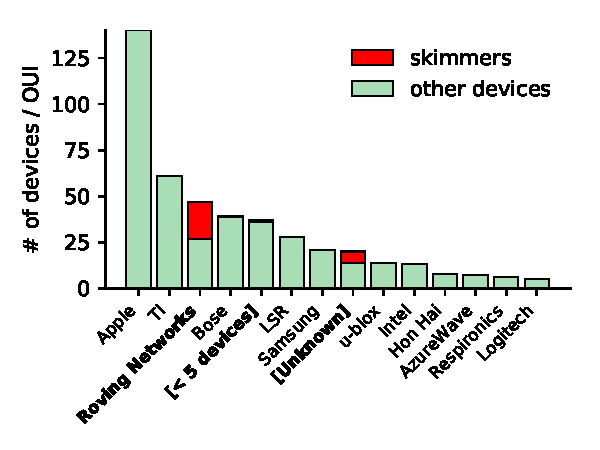
\includegraphics[width=\linewidth]{plots/all_hist_device_OUI.pdf}
%\caption{
%\label{fig:hist_device_OUI}
%Distribution of manufacturers per gas station visit. Skimmers are common amongst Roving Networks and unassigned
%manufacturers, and also occasionally smaller module producers.
%}
%\end{figure}

\begin{figure}
\centering
\includegraphics[width=0.6\linewidth]{skimmer/plots/uncat_hist_device_OUI.pdf}
\caption{
\label{fig:hist_device_OUI}
Many other devices appear to be using the same Bluetooth modules as skimmers.
}
\end{figure}

Within the set of Uncategorized devices, we next look at the distribution of
their MAC prefixes (Figure~\ref{fig:hist_device_OUI}).
%
 %shows the distribution of Unclassified device AC prefixes observed by
%Bluetana at gas stations (listed by manufacturer).
%
We find that the Bluetooth modules used in skimmers are also used in many other legitimate
devices.
%
Specifically, more than half of the RN modules seen at gas stations were in
skimmers, but there were many other devices that had RN modules.
%
%It is possible to identify many skimmers by looking at the MAC address of the
%discovered device and checking it against a hit-list of known skimmer module
%manufacturers.
%
%This hit-list is sourced from reports from law enforcement and previously
%discovered skimmers
%
This is an important observation because a popular detection application,
SkimPlus~\cite{skimplus}, only flags skimmers based on a hitlist of MAC
prefixes~\cite{scaifeoakland}; it may incorrectly flag legitimate devices as
skimmers.

The devices observed with MAC prefixes that were in the \texttt{YY:YY:MM:DD}
format (likely HC modules) were mostly skimmers.
%
There were many devices that had IEEE assigned MAC prefixes that were
infrequently seen at gas stations ($<5$ Devices). Only one of these devices
was a skimmer.
%
Also, there were many devices with MAC prefixes unknown to the IEEE, but not in
the date format, only one of these devices was a skimmer.
%
Overall, \numberBTMACCoDfiltered~devices out of
\numberbtuncategorized~Uncategorized devices matched the MAC prefixes of
Bluetana-observed skimmers.
%Of the devices that had the same MAC prefix as observed skimmers, only
%\numberBTMACCoDfiltered~devices matched these MAC prefixes (out of
%\numberbtuncategorized~Uncategorized devices).
%
This reduces the number of stations where Bluetana detected skimmers to
\visitedstationsMACCoDfiltered~out of the~\totaluncatstation~stations where it found
Uncategorized devices.

%
%It was discovered that this MAC address was questionable after another HC-05
%module close in MAC range had been discovered by investigators.
%
%The device also had a distinctive name which allowed it to be flagged
%independently of OUI.
%
%There were also other devices with MAC prefixes not matching known IEEE assignments, that were not skimmers.
%
%For one of these skimmers, it was clear that the MAC was either purposefully
%misconfigured by the criminal or by the manufacturer of the module.
%
%For all HC-05 modules but two, the MAC addresses were simply the date of
%manufacture in the YY:YY:MM:DD format mentioned earlier.

\if 0 %what is this?
Collaborating with law
enforcement, we were able to develop a hit-list consisting of X addresses. In
fat, there was a case under which we found new manufacturers of skimmers, and
were able to use this new information to isolate skimmers we had seen 7 months
prior. The most common devices that we saw which were of the uncategorized
device class actually ended up being phones; we did not find any skimmers
masquerading as phones. We did see devices with no registered manufacturer. Some
of these were simply odd devices, others were skimmers.
\fi
%}}}

\subsubsection*{Default- and custom-named modules are often skimmers} %{{{

Finally, we investigate if skimmers can be differentiated from other devices by
their Device Name.
%
The remaining~\numberBTMACCoDfiltered~devices are Uncategorized and their MAC prefixes are either: Roving Networks, \texttt{YY:YY:MM:DD}, Unknown, or seen on less than five devices.
%
Only
\totalskimmersfirstvisit~of these devices were confirmed to be
skimmers.\footnote{We do not include 22 of the Bluetana-detected skimmers in
this analysis because they were not detected on the first visit to a gas
station.}
%
In Figure~\ref{fig:hist_device_name}, we divide the remaining devices by their
category of Device Name, including: \emph{unnamed}, manufacturer
\emph{default}, known legitimate \emph{product}, and \emph{customized}.
%
Devices observed by Bluetana with default names were often skimmers.
%
Custom named devices were not common at gas stations but had a higher
probability of being skimmers.
%
Three skimmers were disguised as products, however all three were
distinguishable because their names were popular smartphones, which should not
have the MAC prefix of Bluetooth-to-Serial modules.
%
Bluetana missed capturing the Device Name for many of the skimmers, as well as other
devices that it detected.
%
 
%The relative portion of skimmers each category of  are 22.4\% for Unnamed,
%85.7\% for default, 6.9\% for product, and 33.3\% for custom.
%


\begin{figure}
    \centering
    \includegraphics[width=0.6\linewidth]{skimmer/plots/uncat_visit_hist_device_name.pdf}
    \caption{
    \label{fig:hist_device_name}
    Default and custom names distinguish skimmers from legitimate devices.
    }
\end{figure}


%

%We have seen skimmers disguise their names as cell phones in 3 of our 37 detection cases, and as generic non-malicious
%entities in 4 other cases.
%
%However, as the criminals are not also modifying the OUI of the devices to match, this can actually be used as a clear
%flag that a given device is a skimmer, i.e. seeing a roving networks module advertising itself as a Bluetooth speaker.

%\subsubsection*{Summary}

%In summary, we 

%\todo{We are likely not missing skimmers}

%}}}

%}}}

\subsection{Accuracy of Bluetooth-based Detection} %{{{

To evaluate the accuracy of Bluetooth-based detection, we analyze Bluetana scan
data collected during inspections in Arizona. Specifically, there was a 7-month
time period in which Bluetana was used by many of the Arizona inspectors
(October 7, 2018 -- May 7, 2019), and we compare the reports filed during these
inspections with the scan data that Bluetana collected.

\subsubsection*{Missed skimmers}
\label{sec:falsenegative}

%o measure the accuracy of Bluetooth 

During this time period, there were 27 inspections where
skimmers were found while an inspector was running Bluetana.
%
A total of 42 skimmers were
recovered during these inspections, of which Bluetana was able to detect 36.
%
Therefore, Bluetana missed detecting 14.3\% of the total skimmers recovered during these inspections.

We do not know exactly why Bluetooth-based scanning missed these skimmers.
%
Half of the missed skimmers were from inspections where Bluetana detected other
skimmers at the gas station.
%
It is likely that these missed skimmers were not powered on due to
improper installation.
%
The remaining missing skimmers may have been built with alternate
exfiltration methods, such as SMS~\cite{scaifeoakland}, or even require physical
recovery~\cite{skimreaper2018}.

%Unfortunately, we were unable to test these skimmers in our lab because they
%were sent out to law enforcement immediately for further investigation.
%
	

\subsubsection*{Incorrectly detected skimmers}
\label{sec:falsepositive}

Bluetana highlighted a device in red during 45 Arizona inspections where no
skimmer was found.
%
There were 757 total inspections where inspectors used
Bluetana\footnote{This includes both routine and complaint/prior knowledge
triggered inspections},  Bluetana may have incorrectly detect skimmers in 5.9\%
of inspections.

%Considering Bluetana uses at least MAC prefix and Class-of-Device for
%highlighting, it is likely that these incorrectly classified 

Incorrectly identifying skimmers is likely due to the fact that  RN and HC
modules are used in a variety of legitimate products, some of which are seen in
and around gas stations.
%
We found RN and HC modules in radar-based speed limit signs, weather
sensors~\cite{rnbtweathersensor} automotive diagnostic scanners,
scales~\cite{rnbtscale} and fleet tracking systems~\cite{rnbteletrac}.
%
Some of these devices have Device Names that clearly indicate what product they
are, but would be confused with skimmers if the Device Name
is missing.
%
Unfortunately, several of these products also use the default Device Names on
their Bluetooth modules (\emph{RNBT-xxxx} or \emph{HC-05}).
%
These legitimate devices will look exactly like skimmers.
%
In such cases, inspectors will need to rely on RSSI localization to determine if these devices
are located inside a gas pump.
%}}}

\if 0 % extra text{{{
\subsection{Skimmer Detection Likelihood}
This analysis shows skimmers constitute X number of the visited gas station.

Names:

custom - this many stations (\%)
default - this many stations (\%)
unnamed - this many stations (\%)

The extent to which this characterization will hold true in the coming years, or the extent to which criminals are
developing mechanisms to ``mask'' the fingerprint of their devices is unknown.
%
We include an extended discussion of these factors in section~\ref{sec:discussion}.

Bluetooth detection has additional benefits.
%
In most of the cases in which our application detected anomalous devices, it was able to alert inspectors to skimmers
in pumps which they were not planning upon opening and inspecting.
%
This includes two cases under which the inspectors were simply ``driving by'' a gas station.
%
For five of the skimmers well hidden inside of their pumps, our application was able to determine with confidence
that a skimmer was in the pump despite an initial failed visual inspection.



Additionally, the following discussion does not use Bluetooth Low Energy (BLE) or SDP fingerprinting as detection
mechanisms.
%
BLE introduces complications to potential skimmer discovery which are outside of the scope of this paper.
%
While BLE skimmers have been found in countries outside of the United States, law enforcement in the six states we have
surveyed have not yet come in contact with a device using the protocol.
%
For more details, see section\ref{sec:ble}.
%
Similarly, SDP introduces complications and additional hardware costs which are addressed in section\ref{sec:SDP}.


%\begin{center}
%    \begin{tabular}{r|c|c|c}
%        \textbf{Module} & \textbf{Vendor} & Chip-set & \textbf{Range} \\ \hline
%        RN-\{41/42\} & Roving Networks & CSR 417 & 100m/30m \\ HC-\{05/06\} &
%        \textit{Various} & CSR 417 & 30m \\
%    \end{tabular}
%\end{center}
%
%
%Both modules reported several factory-default fields that uniquely identify
%them, specifically their manufacturer (MAC prefix known as IEEE OID) is a valid
%OID for the manufacturer (Roving Networks). For the HC device which is
%inexpensive, a squatted MAC OID that has not yet been assigned to a manufacturer
%by IEEE. Also, the modules have default Bluetooth names that indicate which
%module they are, and a default device class (i.e., None)---most products have a
%name and device class that reflects the product (e.g., name: ``Bose
%Quiet-Comfort'', class: ``Headphones'').
%%
%Criminals may stick with the default configuration, even though every one of
%these fields can be changed with some hacking (see
%Section~\ref{sec:discussion:hiding}) values because it makes something look
%innocuous.
%
%In summary, the Bluetooth modules commonly found in skimmers may be identifiable
%in Bluetooth scans.
%%
%However, all of the parameters are configurable, and to confirm this hypothesis
%we will need to study skimmers in the wild.
%%
%Designing an Android app to collect this will allow us to study a large number
%of gas stations and collect data on the Bluetooth environment.
%%
%This crowd sourced deployment will allow us to determine if skimmers can be
%reliably detected with Bluetooth inquiry scanning alone.



%\section{Implementation and Overview of Findings}
%
%
%
%To conclude this section, we will give an overview of the effectiveness of
%finding skimmers using the information above.
%
%From the recorded inquiry response data of 115,199 devices and 29,818 unique
%devices near gas stations, we were able to isolate \todo{X} skimmers.
%%
%The primary method used to isolate questionable devices was MAC address
%filtering based upon OUI.
%%
%This method paired with geo-location filtering alone is able to reduce the number
%of potential devices down to 677, at the cost of a potentially high
%false-negative and false-positive rate.
%%
%Not only did this method fail to find two skimmers who OUI's were not in the
%``hit-list'' initially \noteby{MB}{and maybe even more!}, it also flagged a lot
%of non-skimmers which were found to be above suspicion after a manual analysis
%of the other features listed above.

%The prior overview demonstrates the efficacy of combining multiple pieces of scan
%data when finding skimmers.
%%
%In the rest of the paper, we will examine our dataset and discuss the individual
%benefits and drawbacks of each feature listed above.
%%
%From this, we will develop an understanding of how the components work together
%and filter out the noise of the typical gas station environment and detect
%skimmers.

%\todo{NOW THE BELOW IS A SECTION}
%\begin{figure}
%    \centering
%    \includegraphics[width=\linewidth]{plots/cdf_num_devices_seen.pdf}
%    \caption{
%    \label{fig:cdf_num_devices_seen}
%    Distribution of the number of classic and low energy Bluetooth devices seen
%    in a visit to a gas station. Classic devices are far less common than
%    low energy devices.
%    }
%\end{figure}

%We are focusing this discussion only on devices that are Classic Bluetooth,
%because all modules used by recovered skimmers are classic Bluetooth.
%%
%In Section~\ref{sec:ble}, we will describe how Bluetooth Low Energy-based
%skimmers will complicate detection via Bluetooth Scanning.

%\subsection{Collection and Hunt Summary}

%

%\subsection{The Anatomy of a Skimmer Fingerprint}
%
%In this section we will concretize skimmer anatomy based upon those database records which we have confirmed to be
%skimmers and the criminal evidence to which we were given physical access.
%%
%
%Foremost, our understanding of Skimmer anatomy revealed itself in two stages.
%%
%During the initial phase of research, we manually examined each record of our dataset, with a goal of finding the
%offending devices directly.
%%
%Over time, this methodology was refined and automated, and a more sophisticated set of features was analyzed.
%%
%Cases under which this was the case are mentioned explicitly.
%%
%Our interest lies within \textit{characteristics which make skimmers visible, characteristics which help
%skimmers to blend in, and characteristics which criminals could mask}.
%
%The motivating question is: ``can an automated application for skimmer detection be developed?''
%%
%From the following analysis, it should be clear that the answer is affirmative.
%
%\noteby{MB}{Now we look at our pile of skimmers. What is the distribution of MAC addresses, the distribution of
%names, the distribution of skimmers to gas stations, discuss how we were able to localize skimmers in every case in
%which we saw them (report the average minimum RSSI value, [and ideally its distance from the pump but I guess not?]!)
%talk about all the features that are bolded above. Here's some start text.}
%
%Law enforcement have informed us that the two common Bluetooth modules found in
%skimmers are:
%
%\begin{center}
%    \begin{tabular}{r|c|c|c}
%        \textbf{Module} & \textbf{Vendor} & Chip-set & \textbf{Range} \\ \hline
%        RN-\{41/42\} & Roving Networks & CSR 417 & 100m/30m \\ HC-\{05/06\} &
%        \textit{Various} & CSR 417 & 30m \\
%    \end{tabular}
%\end{center}
%
%
%Both modules reported several factory-default fields that uniquely identify
%them, specifically their manufacturer (MAC prefix known as IEEE OID) is a valid
%OID for the manufacturer (Roving Networks). For the HC device which is
%inexpensive, a squatted MAC OID that has not yet been assigned to a manufacturer
%by IEEE. Also, the modules have default Bluetooth names that indicate which
%module they are, and a default device class (i.e., None)---most products have a
%name and device class that reflects the product (e.g., name: ``Bose
%Quiet-Comfort'', class: ``Headphones'').
%%
%Criminals may stick with the default configuration, even though every one of
%these fields can be changed with some hacking (see
%Section~\ref{sec:discussion:hiding}) values because it makes something look
%innocuous.
%
%In summary, the Bluetooth modules commonly found in skimmers may be identifiable
%in Bluetooth scans.
%%
%However, all of the parameters are configurable, and to confirm this hypothesis
%we will need to study skimmers in the wild.
%%
%Designing an Android app to collect this will allow us to study a large number
%of gas stations and collect data on the Bluetooth environment.
%%
%This crowd sourced deployment will allow us to determine if skimmers can be
%reliably detected with Bluetooth inquiry scanning alone.

%\subsection{Feature Analysis}
%
%\subsubsection{Class of Device}
%
%
%\subsubsection{MAC address}


%\subsubsection{Geo-location and Received Signal Strength Indication (RSSI)}
%
%\subsubsection{Persistence} Many of the devices seen during the typical visit are transient, i.e. located in cars
%passing by and at the gas station for only a temporary amount of time; by accumulating records and only recording
%devices for which we receive multiple responses, we can also ensure that we are only selecting devices which are
%persistent at the gas station.
%\noteby{MB}{While we saw an average of X devices per gas station, X of these devices were non persistent, meaning we
%only got one response during the greater-than-a-minute time frame during which we were at the station. Amongst our
%skimmer devices, we got an average of X responses from the skimmer during the visits. This number is inflated by the
%possibility that seeing a skimmer \textit{causes} the investigator to scan more, however, out of the stations at
%which we did not see a skimmer, we saw an average of X persistent devices, indicating that the numbers of responses
%attained from skimmers are in line with the numbers typically seen from persistent devices.}

\subsubsection{Name}

%\todo{Move this section to Discussion}
%\subsubsection{Service Discovery Protocol} Bluetooth also provides the ability to
%query the services that a device can provide without establishing a connection
%to the device, the Service Discovery Protocol (SDP).
%%
%However, as of Android 6.0 the \texttt{BluetoothDevice} method
%\texttt{fetchUuidsWithSdp} will automatically trigger a pairing process with the
%device, making skimmer fingerprinting via SDP infeasible.

\todo{Move the rest of this section and integrate it into the analysis section
with the feature analysis}

The Bluetooth pairing process is most likely familiar due to its prevalence in
consumer electronics. Delving into greater technical detail, however, it follows
the following sequence.

The process begins with a stage called inquiry; this is the primary discovery
stage for Bluetooth enabled worker devices by a master device. The process is
set up in a specific manner to reduce conflict between device scanning, and
speed up discovery so that piconets with a master-worker dynamic can be quickly
set up. In inquiry cycles where the master device is not looking to connect to
devices for a specific purpose or service, the master device, known as the
inquirer, hops among 32 of Bluetooth's 79 1 MHz frequency channels, according to
a pseudo-random pattern seeded by a General Inquiry Access Code (GAIC) defined
within the standard. On each frequency, the device sends out an initial inquiry
packet consisting of the GAIC, a 28-bit CLK for synchronization purposes, and a
unique 48 bit address corresponding to the master device. 625 microseconds after
sending a packet on frequency $x$, the master device will listen on frequency $(x
+ 32) mod 79$ for a response from a possible listening device. Meanwhile, the
listening devices, known as scanners, will listen given frequencies in 1.28
second ``scan windows'', before hopping frequency in a predetermined manner in
order to account for the pseudo-random hopping of the inquirer device. Upon
recieval of the initial inquiry packet from the inquirer device, the scanner
device will begin a back-off based upon a uniformly distributed number of scan
slots between 0 and 1,023, meaning between 0 and (roughly) 640 ms. Once it
returns from this back-off state, the scanner device will begin scanning again,
and wait for a second inquiry packet from the master device. Once this is
received, the device will send out a Frequency Hopping Synchronization (FHS)
packet, in which the inquirer will learn the critical details of the device,
such as unique address. At this point, the inquirer device will finish its
inquiry process, followed by an initiation of paging with the worker device. It
is during this initial paging process that the Bluetooth device name and other
details will be exchanged. But notably, device discovery itself takes around
10.24 seconds in official measurements, and only 5.12 seconds to discover 99\%
of devices, according to more advanced analysis detailed in [Peterson,
Baldwin...].

In order to perform the Bluetooth device discovery detailed within our studies
of gas station environments, we used the Android operating system's
BluetoothAdapter interface to operating system services. A BluetoothAdapter
device discovery cycle typically consists of 12 seconds of inquiry scanning
followed by paging of those devices discovered in order to record device names
and details. There is a tradeoff present within following the default scan
interval; while allowing inquiry to complete ensures that various environmental
factors do not interfere with discovery and information is not lost, in a
crowd-sourced application where localization is a primary concern (in the case
of skimmers, ensuring that the device observed is within a pump), a larger
number of data-points for any given device is of larger concern. Thus, we offered
participants a variable setting for sane defaults between a 5 second scan and
the android default scan time. By restricting the inquiry period to five
seconds, more data-points were retrieved for each device. Additionally, because
paging is handled separately by the system service, this still allowed us to
retrieve device names. It is possible that this led us to miss out on the
discovery of some devices, and eager inquiry scanning to increase the amount of
localization points did interfere with paging, however, it roughly doubled the
number of geo-location points for each observed for each device, allowing for a
more fine-grained discovery of skimmers via the concentric ring based techniques
discussed in a later section. 

\subsubsection*{RSSI is detectably higher in the pump area of the station}

\begin{figure}
\centering
\includegraphics[width=\linewidth]{fig/rssi_motivation.pdf}
\caption{
\label{fig:rssi}
  Combining RSSI data with satellite imagery reveals if a device is located in the pump area of a gas station.
}
\end{figure}

When the skimmer responds to the Bluetooth scan request it responds with a
packet that contains the device's MAC address and class of device, and the
scanner uses the signal strength of this received packet to measure RSSI.
%
By the nature of being installed inside a gas pump, which is often a metal box,
the Bluetooth signal strength is typically only strong in the pump area.
%
Other devices that we suspected may be skimmers, all had a low signal strength
in the pump area, because aside from the cars parked at the pumps, the only
places where a Bluetooth device would be located in the pump area would be
inside the pump.
%
We show this by combining the RSSI with the geo-location from GPS, and satellite
imagery of the gas station, it becomes clear that the inside of a gas pump
(example shown in Figure~\ref{fig:rssi}).
%
While at a gas station this can be seen by moving toward the pump area to see
if the device's signal strength increases. 



\fi %}}}

%!TEX root = paper.tex
\section{Countermeasures and Responses}
\label{sec:hiding}
This work is a single snapshot in an evolving landscape of attacks on payment systems. While Bluetana has
proven effective at finding Bluetooth skimmers, it by no means represents the last move in the cat-and-mouse game. In
the remainder of this section, we discuss what the next few steps in this arms race might look like. That is, given
that inspectors and volunteers are using Bluetana, what can be the skimmer installers' next move, its cost, and what our
response might be. It is possible for a determined and resourceful criminal to implement the countermeasures that we will be describing (particularly non-discoverable mode).


\subsection{Switching to Bluetooth Low Energy}
\label{sec:hiding:ble}

We have observed that by switching to BLE, criminals have \emph{many} more places to hide.
%
Figure~\ref{fig:classic-v-ble} shows the cumulative distribution of the number of BLE and Bluetooth devices we saw at each
fuel station.
%
Under the filtering of Section~\ref{sec:bluetooth}, over 8,000 unique BLE devices were seen, making
the ratio of Classic to BLE approximately 1:4.

\begin{figure}
    \centering
    \captionsetup{justification=centering}
    \includegraphics[width=0.6\linewidth]{skimmer/plots/cdf_num_devices_seen.pdf}
    \caption{BLE devices are more common than Classic.}
    \label{fig:classic-v-ble}
    \vspace{-1em}
\end{figure}

\paragraph{Cost to attacker} There is almost no cost to criminals in switching their Bluetooth modules to BLE.
%
In fact, newer EMV skimmers discovered in other countries are BLE enabled~\cite{krebshimmer}.
%
However, none of our contacts in law enforcement have encountered BLE-based gas station skimmers.
%
It is possible that there is simply no incentive to switch: the same reason criminals have not yet adapted to
masking their Bluetooth device class.

\paragraph{Response} BLE devices may be harder to differentiate due to the higher number of devices at each gas
station and a lack of distinguishing features.
%
With more sophisticated filtering techniques, it may still be possible to isolate BLE skimmers within
this larger set of devices.
%
One possibility is automated RSSI localization to the fuel dispenser location, a possible subject of future research.

\subsection{Non-Discoverable Skimmers}
\label{sec:hiding:desc}

The most natural way to evade discovery via Bluetooth would be to put the module in non-discoverable mode.
%
When a Bluetooth device is non-discoverable, it does not respond to normal Bluetooth scans.
%
Instead, it only responds to paging packets specifically addressed to its MAC address.

\paragraph{Cost to attacker} Non-discoverability would make exfiltration more difficult for criminals.
%
One possibility is creating a pre-paired data collection device.
%
However, we have been informed by law enforcement that the individual who installs the skimmer is often independent
from the individual responsible for data recovery (called a ``mule'').
%
The criminal would not be able to send a mule to recover card data without first delivering them the device.
%
Alternately the criminal could record the MAC address of the skimmer Bluetooth module.
%
This would require careful bookkeeping and the use of tools that support the creation of a non-discoverable connection.

\begin{comment}
    The downside of pre-pairing and making the device non-discoverable is that the device
    becomes visible \emph{only} to the host with which it was pre-paired. This means that the person sent to collect the
    skimmer data must have the same host device with which the skimmer has been paired before installation. Moreover, if
    this host device is lost or becomes nonfunctional, all access to the skimmer is lost. The installer would need to
    physically access the skimmer to initiate pairing again, which carries nearly the same risk as installing a new
    skimmer.
\end{comment}

\paragraph{Response} It is still possible to discover a non-discoverable device.
%
For a small set of target address ranges, e.g., \texttt{00:06:66} used by Roving Networks modules, we believe it
would be practical to attempt to guess all 16.8 million possible addresses.
%
Prior work has shown that it is possible to discover any non-discoverable device via brute force in 18.64 hours;
knowledge of OUI would ideally allow us to reduce this search time~\cite{cross2007detecting}.
%
Unfortunately, this requires specialized hardware, rather than an inexpensive Android phone.

\subsection{Impersonating Common Benign Devices}
Another natural response to Bluetana would be to change the MAC address and name of the device to that of a common
benign device, such as a mobile phone or a Bluetooth-enabled car entertainment system. This would make the skimmer
appear innocuous to Bluetana.

\paragraph{Cost to attacker} Reprogramming the MAC address on the CSR-based Bluetooth modules, which include the
Roving Networks and HC-05 and HC-06 modules, cannot be done using the AT commands used to change device name and
pairing. Instead, the skimmer installer would need to re-flash the CSR firmware using a special programming cable.
While, in principle, not difficult, it would require an additional degree of sophistication than programming a simple
micro-controller development board. The skimmer installer could also change the device name but not the MAC address,
say, to one of the known benign devices using the same module, something that us possible to do by issuing AT
commands from the micro-controller to the module. While this may cause Bluetana to detect these as a skimmer, signal strength can still be used to identify location of the module.

\paragraph{Response} Because Bluetana collects all Bluetooth data, we can identify skimmers retroactively when we
learn of a new MAC address and name used by known skimmers. Thus, if attacks switch to impersonating benign devices,
we can update the Bluetana highlighting mechanism to identify those devices as suspicious. This would result in
additional inspections, but would still provide significant gain over the state of the art.

\subsection{Using Non-Bluetooth Communications}
During discussions with law enforcement agencies tasked with identifying skimmers, we were told about skimmers that
use GSM modems or WiFi as an alternative to Bluetooth. In the case of WiFi, we believe that the Bluetana methodology
will still be effective. GSM poses a more serious challenge for detection.

\paragraph{Cost to attacker}
While using GSM would avoid detection using Bluetana, it creates an additional trail of evidence linking the
perpetrator to the skimmer. Law enforcement officers could obtain information about the SMS recipient through
subpoenas, so receiving the SMS messages on another phone on a US carrier, for example, would be easy to trace.The
perpetrator would need to use an SMS service that would not expose his/her identity.

\paragraph{Response} In addition to legal tools available to law enforcement to trace SMS messages, a GSM modem could
be detected using a Software-Defined Radio.% including a low-cost (\$10) RTL-SDR dongle.

\subsection{Attacker Bottlenecks}
The attacker (skimmer installer) has several practical ways to evade detection using Bluetana. Each of these, however
, has an additional cost in terms of effort, risk exposure, or expertise. We do not yet have a strong
understanding to which of these costs attackers are most sensitive. Indeed, the very low price of stolen credit card
numbers, compared to their potential cash out value (Table~\ref{tab:cardval}) suggests that the bottleneck in the
carding value chain is \emph{not} getting card information but cashing out cards. Thus, while Bluetana may raise the
cost for attackers, we do not believe that it will raise it so much as to make fuel dispenser skimming unprofitable.

%!TEX root = paper_main.tex
\section{Operational Lessons Learned}

While performing the Bluetana study, we learned several lessons about the
operational use of Bluetooth scanning for skimmer detection. In this section,
we provide an overview of two most important lessons we learned.

%\subsection{False positives happen, but they do not waste too much time and Few skimmers can not be detected with Bluetooth}

%\todo{finish this}

%Peterson et al.~\cite{peterson2006bluetooth} showed that 99.98\% of devices can be discovered in 6.4 s of inquiry time. This matches the observation of our measurement study, that presence of Bluetooth skimmers can be determined in a short amount of time without performing time consuming manual inspections. During the course of our study, we also saw another interesting consequence of the short time of discovery - investigators can discover presence of skimmers while simply driving by gas stations.

\subsection{Bluetooth Helps During Inspections}

Criminals hide skimmers in the crevices of gas pumps to avoid detection during inspections.
%
We witnessed several instances where investigators were unable to locate skimmers via physical inspection alone. 
%
In one incident, Bluetana flagged four devices at a station; however, no skimmers were located.
%
This result led officials more experienced in skimmer recovery to perform a second thorough inspection of the station.
%
These officials located all four skimmers.
%
The evidence provided by Bluetana forced them to continue the inspection, instead of abandoning it and leaving the devices in the field.

\begin{figure}
    \centering
    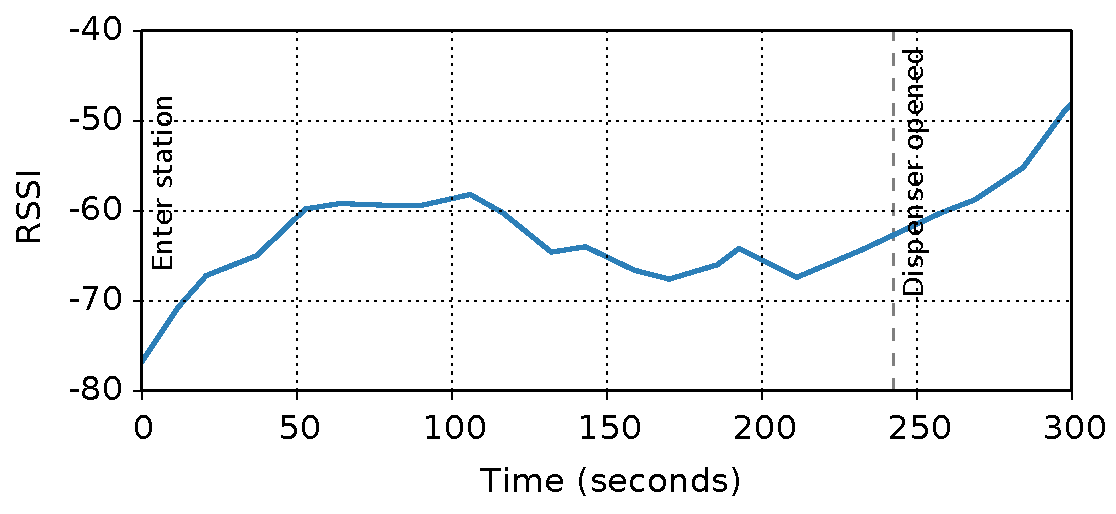
\includegraphics[width=\columnwidth]{skimmer/plots/rssi_jump.pdf}
    \caption{
    \label{fig:rssi_jump}
  Opening of the gas pump enclosure results in a significant jump in observed Bluetooth
  signal strength from a skimmer. 
    }
\end{figure}



Figure~\ref{fig:rssi_jump} demonstrates an instance of how the signal strength
measurements helped inspectors determine which pump had a skimmer. When the gas
pump's metal door was opened, the signal strength increased significantly,
prompting inspectors to look carefully for the skimmer in that pump.

\subsection{MAC Addresses May Indicate the Source}
\label{sec:ops:macs}

\begin{table}
\centering\small
\begin{comment}
\begin{tabu} to \linewidth {lrrrrrr}
\toprule
  \textbf{Group} & \textbf{1} & \textbf{2} & \textbf{3} & \textbf{4} & \textbf{5} & \textbf{6} \\
\hline
No. of skimmers & 2 & 2 & 2 & 2 & 5 & 3 \\

Seen across stations & 1 & 1 & 2 & 2 & 2 & 2\\

Min. distance in MAC address & 17 & 166 & 9 & 3 & 4 & 4 \\

Min. distance between & & & & & & \\
closest MACs (miles) & 0 & 0 & 17 & 17 & 17 & 448 \\
\bottomrule
\end{tabu}
\end{comment}
\begin{tabu} to \linewidth {lrrrrr}
\toprule
   & \multicolumn{5}{c}{Group} \\
   \cmidrule(lr){2-6}
   & \textbf{1} & \textbf{2}  & \textbf{3} & \textbf{4} & \textbf{5} \\
\hline
Skimmers & 3 & 5 & 6 & 4 & 3 \\

Gas stations & 2 & 2 & 5 & 4 & 2\\

Min. difference in MACs & 1 & 4 & 9 & 10 & 4 \\

Closest MAC distance (in miles) & 0 & 17 & 59 & 203 & 448 \\
\bottomrule
\end{tabu}

\caption{Several geographically separated skimmers had similar MAC addresses.}
\label{tab:mac_closeness}
\end{table}

Network equipment vendors (e.g., Bluetooth module manufacturers) tend to allocate MAC addresses sequentially by production time~\cite{wifi-macs}.
%
Therefore, if two devices have similar MAC addresses, they are likely part of the same batch of devices sold.
%
This information can be used to associate skimmer Bluetooth modules to the same board designer or crew.

We group the skimmers found by Bluetana with the same first 5 bytes of MAC address.
%
Table~\ref{tab:mac_closeness} shows five such groups.
%
We list the difference in MAC address and the geographic distance between the closest MACs in each group.
%
Skimmers in group 1 and 2 were recovered at gas stations in the same county, separated by at most 17 miles.
%
From LE sources, we know that criminals often plant skimmers across multiple stations in a given city/county, and the MAC address data collected indicates this.
%
Groups 3-5 are the most interesting, as the closest MACs in the same group are in stations across different counties.
%
The closest MACs in group 5 are at stations separated by 448 miles.
%
This may seem surprising, but LE informs us that skimmer crews avoid detection by migrating from city to city. 

%%!TEX root = paper.tex
\section{Discussion}
\label{sec:discussion}

\subsection{Why we think we are not missing skimmers} %{{{

Throughout the course of this study, we have been in direct communication with government officials from numerous states
responsible for the removal of skimmers, and have developed a working relationship wherein we are notified any time
a new breed of skimmer appears which is currently undetected by the Bluetana application.
%
Thus, our ability to detect skimmers depends upon the current level of investigation performed by government officials;
%
if a skimmer using a new OUI previously unflagged were to be discovered at a gas station by any of the 40+
investigators, it is likely we would be notified.
%
In fact, this has already occurred.

This lends confidence to our measurements and analysis \textit{at the current point in time}.
%
In the coming years, criminals may make a shift to using other technologies, i.e. radio, to retrieve data from
skimmers.
%
Now we will discuss ...
%}}}

\subsection{Countermeasures} %{{{

\subsubsection{EMV}
\label{sec:discussion:emv}

Credit card companies will soon require upgrading magstripe terminals to to EMV
chip technology \todo{cite}.
%
Although there are fewer vulnerabilities with EMV cards, namely the attack the
exposed reader cabling attack vector, that brought on internal skimmers
\todo{cite}.
%
There are obvious concerns on if this is realistic, as gas stations operators
were required to upgrade fuel dispensers to the new EMV-based card readers by
2018, but the deadline was extended but the large number of gas stations makes
it prohibitively expensive to do so, and therefore the deadline was extended.

Already, criminals have productised EMV versions of internal skimmers, called
deep-insert skimmers, or ``shimmers''.
%
Deep-insert skimmers bear striking resemblance to the magstripe internal
skimmers.
%
The reason is, both magstripe and chip card readers transfer card information
over a digital serial bus.
%
However, instead of tapping into the serial signal at the exposed cabling, EMV
skimmers are inserted fully into the cardslot.
%
Newer EMV chip cards obviate the need for an analog decoder by directly
providing the digital serial interface.
%
If you tap into an EMV signal you can still produce a mag-stripe card and use
it somewhere else \todo{cite}.

% \begin{figure}
% \centering
% 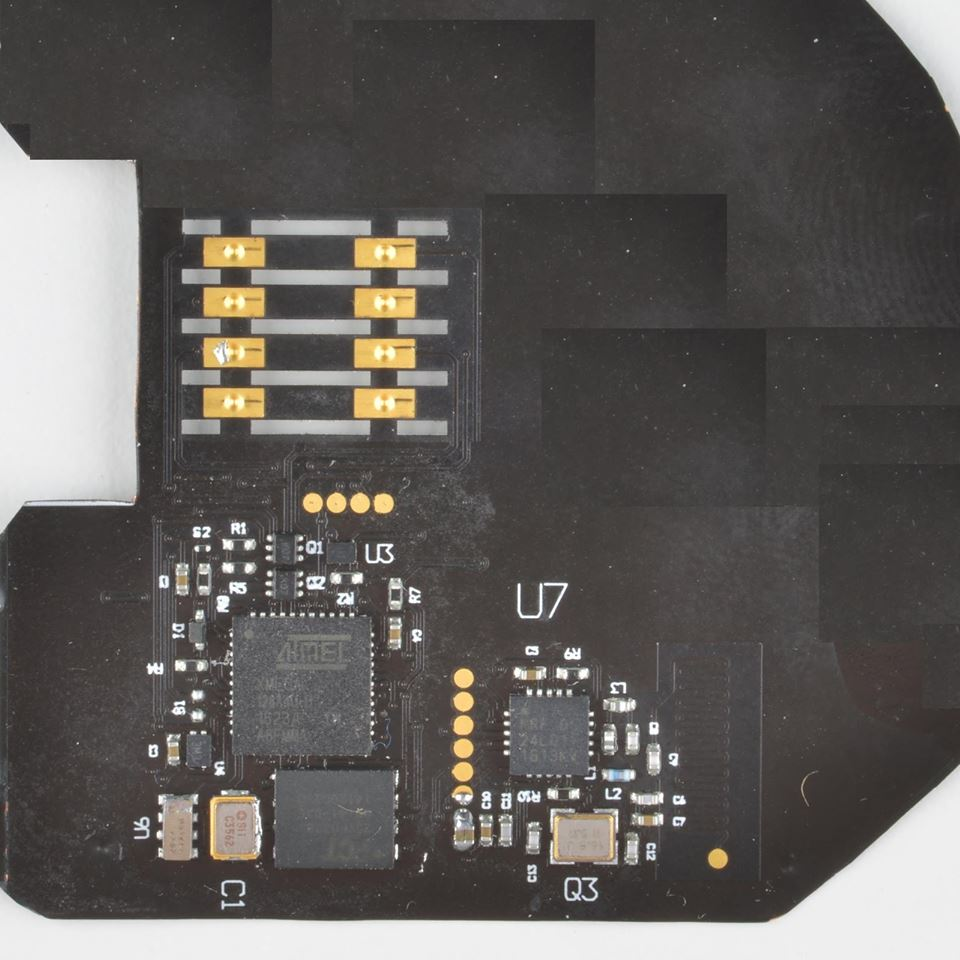
\includegraphics[width=0.5\linewidth]{fig/deep-insert}\\
% \small{Image source: gas-pump-skimmer.com}
% \caption{
% \label{fig:deep-insert}
% A ``Deep-insert'' EMV chip skimmer with wireless (Bluetooth Low-Energy) exfiltration capability.
% }
% \end{figure}

Figure~\ref{fig:deep-insert} shows an example of a deep insert skimmer that
demonstrates they are just a new version of internal skimmers in that they
passively capture card information, and they have a wireless interface for
exfiltration.

% https://link.springer.com/chapter/10.1007/978-3-642-04904-0_7
%}}}

\if 0 %{{{

\subsubsection{Physical security}
\label{sec:phys-security}

Although it would appear that card security was not a priority in the design of
fuel dispensers, the PoS circuit encrypts all payment information in transit to
the central payment processing unit in the gas station.
%
Rather, the security measures did not protect against tiny embedded system
could be installed inside the enclosure and exfiltrate the data wirelessly.
%
This is also indicated by the poor physical security in enclosure designs that
could have stopped criminals from gaining access into the internal circuitry.
%
Details about the physical security vulnerabilities of fuel dispensers are
discussed in Section~\ref{sec:phys-security}. 

\begin{figure}
\centering
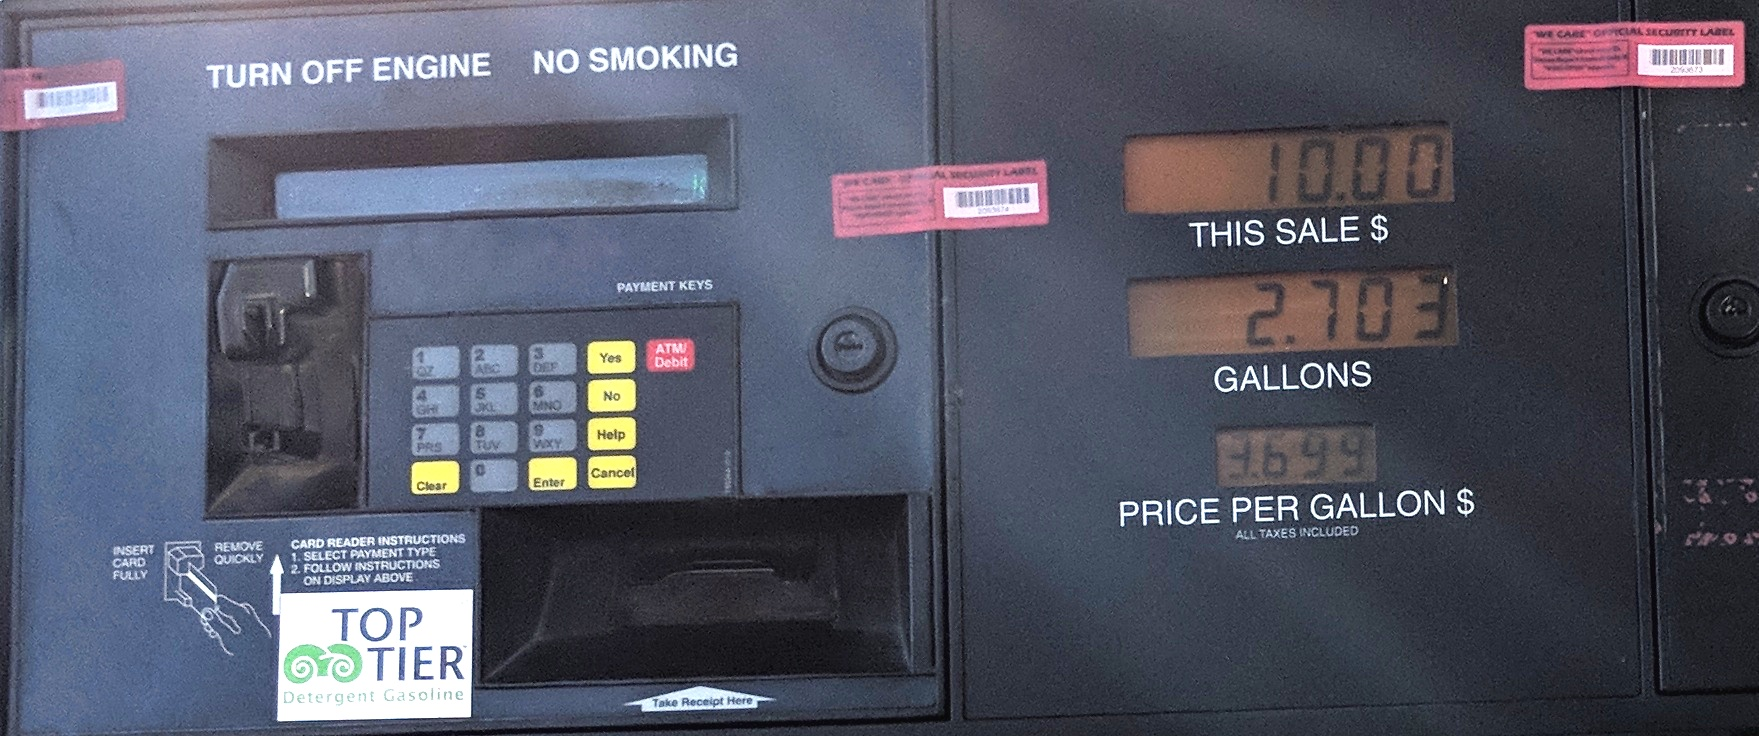
\includegraphics[width=\linewidth]{fig/tamperseal-pump.jpg}
\textbf{Multiple tamper-evident seals on a dispenser.}\\
\vspace{0.2in}
\fbox{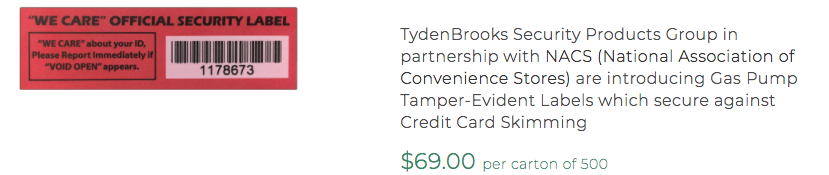
\includegraphics[width=\linewidth]{fig/tamperseal.png}}\\
\textbf{Identical seals can be purchased online.}
\caption{
\label{fig:tamperseal}
Criminals can easily replace voided seals.
}
\end{figure}

\paragraph{Tamper-evident seals}
%
Criminals also have to bypass any tamper-evident seals that the station owner
attaches to the dispensers.
%
In theory tamper-evident seals should deter criminals from installing skimmers.
%
However the significant effort required to maintain tamper-evident seals at
fuel stations makes them cumbersome to use.
%
An attendant must replace the seals every time the dispenser is inspected and
serviced.
%
Interestingly, some stations even install multiple seals with the intention of 
improving security, however this only makes it more difficult to check
if a criminal has replaced the seal with a new seal that has a different serial
number (Figure~\ref{fig:tamperseal}).
%
As such, we have found many tamper evident seals at gas stations are cut or
activated.
%
As further evidence of how ineffective security seals are, replacement security
seals were found in the possession of criminals that were arrested while they
were installing a skimmer~\cite{texas_criminal_security_seal}.





As described in the sections above, Bluetana has been and continues to be an effective weapon in the law enforcement fight against skimmers in the wild. Our methodology essentially uses characteristics of commodity Bluetooth devices in skimmers to be able to detect them. As details of our methodology become public, criminals will try to adapt to prevent skimmer detection. Based on knowledge gathered over the course of our research, in this section we try and analyze possible modifications that can be made to current skimmers to make detection more challenging, and whether Bluetana measures up. We also try to present this section as a lookahead of how the skimmer landscape might evolve in the future and thus present this as a point of reference for future work in the area.

Q : Why dont the criminals simply migrate to a longer range wireless communication mechanism like cellular?

A : By the looks of it, for a skimmer application cellular seems to be a good fit. Criminals are saved from the burden of having to drive to gas stations to collect data, thus putting more distance between them and the scene of the crime. Cellular radios however add an extra cost of requiring to purchase a SIM card with an active cellular plan. Cellular radios themselves are in general costlier than commodity Bluetooth modules and thus overall skimmer cost goes up. Addtionally, when recovered, presence of an active cellular connection can give law enforcement a much easier investigative route to pursue the criminals. Consequently, added cost and higher risk make cellular radios less likely to be used for skimmers in the future

Q : Well if not cellular, what about other wireless radios

Q : Gas pumps are now migrating to chip based readers which they are secure, so this wont be a problem in the long run, right ?

A : Not so much. Most current migration is cosmetic. Replacing entire CRIND tray mechanism or buying new machines is costly, and so current chip based modular replacements, simply read data from the cards but transmit to the backend POS in the clear. Even if we consider the case that new models of pumps based on chip readers are installed, chip based EMV mechanism has been found to be vulnerable to replay attacks because of weak RNG [cite IEEE paper]. In fact, ingenous skimmers already exist in the market that take into account these weaknesses and are able to bypass SDA, DDA and CDA to create a data dump that can be used to create perfect clones [cite website for skimmer]. However, the idea of using wireless radios to ease in the data collection and reduce chances of getting caught, are still valid and will hold. Hence focussing on this interface as a means for detection will continue to stay valid. Case in point, the chip skimmer also has a Bluetooth radio onboard

Q : A major component of your paper has been the idea of crowdsourcing, and yet you only collected data for the survey using a few individuals?

A : The idea of multiple individuals using the toolkit to detect skimmers in a large geographic area does remain valid. During development of this toolkit, we were concerned about details of our method leaking to criminals, and thus it was important to keep the circle of trusted individuals small, and thats why we the authors took to scanning the gas stations ourselves. We are in conversation with multiple state level Weights and Measures and local PDs, and will soon have large scale crowdsourcing in place. However, the fact that only a few individuals scanning for skimmers at gas stations were able to recover 10 odd skimmers, does tend to lend credence to the argument that with a large scale deployment, we will have signifantly greater capture rates

\begin{enumerate}
\item  Unnamed Devices are a limitation
\item   We use the MAC address, other metrics in that case
\item   Method in field relies more on the hitlist
\item     Hitlist can be comprehensive
\item     Using data from police recovery, as well scraping of
    websites like alibaba, sparkfun, digifruit, ebay, ...
\item    	      Incremental; if a new device shows up and
	     we are notified, we can rerun metric analysis to
	     find the new hitlist devices
\item	      method is extendable
\item What about randomized MAC addreses / smarter skimmer
\item   Full randomization, the criminal must rely on the device name
  to recover the device, since the person that is extracting the
  data is not the same as the one that implanted. Crims generally
  use mules, according to law enforcement agencies.
\item   Now, there can be a limited randomization, in which you use
  a pool of MAC addresses
\item     This is more sophisticated, and damages our methodology, the
    mitigations for this are more complicated but come in one of
    two forms: either persistent monitoring devices at each gas station
    or an even larger crowd sourced approach, wherein you get enough coverage
    of each gas station to determine persistence
\item        This is more difficult to detect. You could flag based upon whether
       the MAC address device is abnormal compared to a baseline for other
       gas stations: if you see a thermostat, it is bad.
\item        But even apple uses 47 bits of randomization, trampling upon other
       manufacturers, so how do you tell this is not another consumer
       electronic, or that the criminal is not masquerading as a common
       bluetooth device, i.e. a Tile?
\item  So consider the case of a smart criminal (i.e. one of the authors of this
paper) designing a skimmer. They would randomize the fingerprint so that
it looks like one of 255 tiles.
\item    In a largescale crowdsourced approach, you might, in the best case,
   have someone come by and scan the gas station every 3 hours. Using our
   methodology, this would not flag odd name, bad MAC, seen twice ... 
\item    There is still a possibility! For each gas station, record the geoloc
   of each of the pumps. For each gas station, check the rssi of the devices
   scanned, and see get a high confidence localization inside the pump. From
   multiple datapoints, you should be able to determine whether the bluetooth
   device is inside of a pump, and there are no bluetooth devices commonly found
   inside pumps.
\item    and you can't spoof RSSI. It is approximate, and depends on the phone/reciever
\item    Since each phone has a subjective perspective, to get the ground truth, you
   would localize to a centroid for each observer, and then combine these centroids
   to localize the skimmer.
\item    Thus, even if criminals were not dumb, we could find them.
\end{enumerate}
\fi

%}}}

%!TEX root = paper.tex
\section{Related Work}
\label{sec:relatedwork}
\paragraph{Skimmer Detection and Prevention}

In recent work, Scaife et al. surveyed gas pump skimmer detection and
prevention mechanisms~\cite{scaifeoakland}.
%
They found that several popular Bluetooth-based skimmer detection applications
use a only MAC prefix or device name matching.
%
The results of our study show how the Bluetooth profile of skimmers in these
applications can be improved to detect more skimmers, and to flag fewer
legitimate devices as skimmers.
%
We also find that Bluetooth-based scanning is an effective way to augment
manual gas pump inspections.
%
Scaife et al. also introduced SkimReaper~\cite{skimreaper2018}, an effective
tool for detecting external skimmers.
%
SkimReaper is a credit-card shaped device that an official can swipe in a card
reader to detect if the reader has an additional read head: indicating that the
reader has an external skimmer attached to it.
%
%This tool detects the presence of a second read head capturing card data in a
%card reader.
%
%Physical contact makes it possible to build a circuit which reveals the
%presence of a second read head.
%
However, SkimReaper can not detect internal skimmers because they do not
add an additional read head.
%
Additionally, the PCI Security Standards Council have released guidelines for
preventing external skimming~\cite{skimmingprevention}.
%
Criminals may start using Bluetooth to retrieve card data
from external skimmer. If they do, we
demonstrate that Bluetooth scanning can augment
these existing external skimmer detection and prevention methods.
%
%Wireless scanning makes the discovery internal skimmers possible without
%manual inspection.
%
%
%Bluetana presents an intermediate stopgap to internal skimming; however, more
%work on preventative measures is needed.

\paragraph{Bluetooth}

Prior work has evaluated the effectiveness of Bluetooth scanning for detecting
and localizing Bluetooth devices.
%
They found that Bluetooth signal strength (measured by an Android smartphone)
is effective for localizing Bluetooth
devices~\cite{liu2014face,wang2013bluetooth}.
%
This work inspired us to use signal strength to detect if a Bluetooth device
appears to be installed inside of a gas pump.
%
Previous studies also examined how long it takes to detect a Bluetooth
device from stationary observers and moving vehicles.
%
They found that Bluetooth devices are often detected in less time than the
Bluetooth standard suggests~\cite{murphy2002using,
peterson2006bluetooth,haartsen1998bluetooth}.
%
This work supports our findings that skimmers are often discovered within the
first few seconds of passing by a gas station.
%
%It also demonstrates the usefulness of drive-by scanning in Bluetooth skimmer
%discovery.

\paragraph{Inventory Attacks}

Prior work has demonstrated that user privacy can be violated by inspecting the
characteristics of a user's device~\cite{ziegeldorf2014privacy}.
%
These so called \emph{inventory attacks} have been demonstrated for Bluetooth
Low-Energy, RFID, and even web browsers~\cite{van201050,
vastel18fp,fawaz2016protecting}.
%
Our work demonstrates a Bluetooth-based inventory attack against malicious
devices, can be used to protect the privacy of consumers.

%\paragraph{Payment Processing Security} Credit card spoofing and transaction
%fraud is a common area of research; while criminals currently rely on the
%trivial vulnerabilities of magnetic strips \cite{magspoof}, it is conceivable
%that newer systems (such as Chip-and-PIN) will prevent magnetic strip based
%attacks. Card issuers feel that removing sensitive data from the magnetic strip
%on cards will help to solve the problem \cite{pcidss}. However, newer literature
%has demonstrated attacks on chip, NFC, and tokenized payment systems
%\cite{bar2005known} \cite{bond2014chip} \cite{roland2013cloning}
%\cite{bai2017picking}. In response to the growing popularity of chip-based
%systems, criminals have begun to develop shimmers: chip-based deep-insert
%Bluetooth-enabled skimmers powered by the EMV reader itself
%\cite{krebshimmer}. The nature of shimmers (Bluetooth) indicates that wireless
%data exfiltration will continue to be an issue. Criminals will always be
%motivated to integrate wireless exfiltration mechanisms as physical retrieval
%involves a risk of being caught. It follows that work on wireless-based
%detection mechanisms like Bluetana will continue to be relevant as vendors
%transition to newer payment mechanisms.  \footnote{This discussion disregards
%the use of vendor-specific payment apps, such as those which have been devised
%by Shell \cite{shellapp}, as these network-based mechanisms come with a host of
%other problems which are outside the scope of this paper.}

%!TEX root = paper.tex
\section{Future Work and Conclusion}
\label{sec:conclusion}

As new skimmer detection tools gain popularity, criminals will adapt skimming designs to evade detection.
%
We expect future skimmers will use techniques such those described in Section \ref{sec:hiding}.
%
Similar to Bluetana, future work in this area should emphasize designing easy-to-deploy systems for detecting
skimmers, and evaluating their effectiveness with large-scale studies.

Push-back from banks and card issuers has led to wide-scale adoption of EMV in
retail PoS systems. 
%
However, EMV adoption in gas stations across the U.S. has been slow due to high
costs.
%
Therefore, Visa and Mastercard have pushed the EMV adoption deadline for gas
stations from 2017 to October 2020~\cite{emv2020}. 
%
As gas stations begin migrating to EMV, skimmers targeting EMV will become more
common. 
%
Future research should focus on the detection of EMV ``shimmers'' that are
gaining in popularity.

Finally, we believe gas pump skimming is the harbinger of an era of attacks
using illicit wireless access links. 
%
For example, there is an internal Bluetooth-based implant for unlocking door
access control systems~\cite{blekey}. 
%
Future work should also identify other
systems that are vulnerable to using such illicit links.

In this chapter, we presented results of a 19-month-long measurement study of
Bluetooth scanning as a mechanism to detect illicit internal gas pump skimmers. 
%
Our evaluation showed that link layer characteristics of Bluetooth-based internal skimmers
can be distinguished from other Bluetooth devices commonly seen at gas
stations. 
%
We detected, and LE recovered, \totalskimmers~skimmers at 34 gas
stations across four states in the U.S. 
%
For \totalskimmersBluetana~of the detected skimmers, Bluetana was the only
source of information that prompted investigators to conduct an inspection.
%
In conclusion, link-layer information revealed in Bluetooth scans is effective at detection of illicit wireless access links at public locations, even in the presence of tens of other Bluetooth devices.

\begin{comment}
This paper presented Bluetana, a empirical measurement study of Bluetooth's ability to detect internal
card skimmers. Bluetooth makes it possible to quickly and accurately detect skimmers within gas dispensers.
Our evaluation has shown that Bluetooth is a promising method of skimmer detection, capable of
detecting ~\totalskimmers~ skimmers for a \emph{daily} monetary impact of ~\Bluetanafraudprevented~ dollars in a study of ~\visitedgasstations~ stations.
\end{comment}

%
\begin{comment}
However, gas stations have not adapted.
%
We randomly sampled 0.5\% of all gas stations in the US and classified pump payment technology.
%
Google Street View images of the dispensers revealed that as of the current date only 13.8\% of gas stations have
retrofitted EMV readers and only 1.6\% have installed EMV based dispensers.
\end{comment}

%%!TEX root = paper.tex

\section{Acknowledgements}
\label{sec:acknowledgement}

We would like to thank our shepherd and the anonymous reviewers from IEEE
S\&P 2022 for their insightful comments. We also thank the reviewers from MobiSys
2021 and USENIX Security 2020 whose feedback lead to this manuscript.
Also, thanks to Stefan Savage for his helpful comments.
%
This work was supported by in part by Qualcomm's Innovation
Fellowship, and a gift from Amateur Radio Digital Communications.

%%!TEX root = paper.tex

\section{Modified Results}
\label{sec:mod_bluetooth}

In this section, we present the results of our 19~month study of Bluetooth
devices observed with Bluetana at ~\visitedgasstations~ gas stations across six U.S.
states (CA, AZ, NV, MD, IL, NC).
%
During the course of this study, Bluetana detected \totalskimmers~skimmers operating in \Bluetanaskimstations~gas
stations; all of the skimmers were removed from the pumps by local and
federal law enforcement agents.
%
Bluetooth scanning is a surprisingly effective way of detecting skimmers: in
Arizona, Bluetana has detected skimmers at 1.58\% of the \visitedgasstationsAZ~stations it
scanned, and routine inspections by state
inspectors had a similar detection rate of~\azpercentskimfound~from 2016 to 2018.
 
The primary result of this study is as follows: there are distinct characteristics of the
~\totalskimmers~internal skimmers detected by Bluetana that differentiate
them from the 2,562 other Bluetooth devices that Bluetana found 
at gas stations (e.g., car stereos).
%
Namely, these skimmers were predominately using the default Bluetooth module configuration.
%
Additionally, we discovered that some criminals use a custom Device Name 
in an apparent attempt to hide their skimmers from Bluetooth scans.
%
We found that these custom Device Names stand out, making these skimmers easier to differentiate from other devices.

%Simply filtering by the~\visitedgasstations~gas stations to those that have devices matching two properties of skimmers---their
%Class of Device and their MAC prefix---leaves only \visitedstationsMACCoDfiltered~stations.

%, out of \visitedgasstations~gas.
%
\begin{comment}
Additionally, we discovered that the only technique that criminals use today to
do to hide skimmers in Bluetooth scans---using a custom Bluetooth device
name---actually makes it easier to differentiate the skimmers from other
devices. \noteby{MB}{We now know this not to be completely true...}
\end{comment}
%
\begin{comment}
surprisingly, one station was infected with skimmers twice during the
course of the study, and two skimmers were still installed six months after we initially detected them\footnote{These skimmers were discovered by looking back at our dataset after we discovered a new way that skimmers appear in Bluetooth scans.}.
\end{comment}
%
%Surprisingly, 81.3\% of
%these devices appear to be legitimate products that use the same Bluetooth
%modules that criminals use in skimmers (e.g., engine diagnostic monitors).




\subsection{What Do Skimmers Look Like in Scans?} %{{{
\label{sec:bluetooth:skimmers}

\begin{table}
    \centering\small
    \begin{tabular}{lll}
    \toprule
    & \multicolumn{2}{c}{\colname{\# of skimmers}}\\
    \cmidrule(lr){2-3}
    \colname{Bluetooth Scan Property} & \colname{Bluetana}  & \colname{LE}\\
    \hline
    \textbf{Class-of-Device} \\
    \quad Uncategorized & 64 & 23 \\
    \hline
    \textbf{Manufacturer (MAC prefix)} \\
    \quad Roving Networks \\
    \quad \quad \texttt{00:06:66} & 45 & 13 \\
    \quad Shenzhen Bolutek \\
    \quad \quad \texttt{98:D3:31} & 1 &  \\
    \quad \textit{Unknown}  \\
    \quad \quad \texttt{20:13:04} & 1 &  \\
    \quad \quad \texttt{20:17:11} & 1 &  \\
    \quad \quad \texttt{20:18:01} & 2 &  \\
    \quad \quad \texttt{20:18:04} & 1 &  \\
    \quad \quad \texttt{20:18:07} & 1 &  \\
    \quad \quad \texttt{20:18:08} & 4 & 10 \\
%    \footnote{The HC-05 modules skimmers use have MAC addresses which
%    are configured at manufacturing time to match the date.}
    \quad \quad \texttt{20:18:09} & 4 &  \\
    \quad \quad \texttt{20:18:10} & 1 &  \\
    \quad \quad \texttt{20:18:11} & 2 &  \\
    \quad \quad \texttt{98:D3:35} & 1 &  \\
    \hline
    \textbf{Device Name} \\
    \quad \textit{Default} & 36 & 23\\
    \quad [Law enforcement] & 2 & \\
    \quad [Mobile phone] & 4 & \\
    \quad [Indescript object] & 2 & \\
    \quad [Numerical] & 2 & \\
    \quad \textit{Unnamed} & 18 & \\
    \midrule
    \midrule
    \textbf{Total} & 64 & 23 \\
    \bottomrule

\end{tabular}

\begin{comment}
\begin{tabular}{lll}
    \toprule
    & \multicolumn{2}{c}{\colname{\# of skimmers}}\\
    \cmidrule(lr){2-3}
    \colname{Bluetooth Scan Property} & \colname{Field}  & \colname{Officials}\\
    \hline
    \textbf{Class of Device} \\
    \quad Uncategorized & 37 & 23 \\
    \hline
    \textbf{Manufacturer (MAC prefix)} \\
    \quad Roving Networks \\
    \quad \quad \texttt{00:06:66} & 27 & 13 \\
    \quad Shenzhen Bolutek \\
    \quad \quad \texttt{98:D3:31} & 1 &  \\
    \quad \textit{Unknown}  \\
    \quad \quad \texttt{20:13:04} & 1 &  \\
    \quad \quad \texttt{20:17:11} & 1 &  \\
    \quad \quad \texttt{20:18:01} & 2 &  \\
    \quad \quad \texttt{20:18:08} & 3 & 10 \\
    \quad \quad \texttt{20:18:09} & 1 &  \\   
%    \footnote{The HC-05 modules skimmers use have MAC addresses which
%    are configured at manufacturing time to match the date.}
    \quad \quad \texttt{98:D3:35} & 1 &  \\
    \hline
    \textbf{Advertised Name} \\
    \quad \textit{Default} & 21 & 22\\
    \quad [Law enforcement] & 2 & \\
    \quad [Mobile phone] & 2 & \\
    \quad [Indescript object] & 1 & \\
    \quad [Numerical] & 2 & \\
    \quad \textit{Unnamed} & 9 & 1\\
    \midrule
    \midrule
    \textbf{Total} & 37 & 23 \\
    \bottomrule

\end{tabular}
\end{comment}

    \caption{Bluetooth scan properties of skimmers observed during our study.
    %
    The exact Device Names are not shown, instead we describe the names we found.
    }
    \label{tab:skimmer-data-overview}
\end{table}


We begin by presenting how skimmers we observed appear in Bluetooth scans.
%
We describe the properties of two sets of skimmers: \totalskimmers~skimmers that we detected in the field
during the course of this study, as well as \totalskimmersLE~skimmers that were independently recovered by two LE agencies.
%
The \totalskimmersLE~skimmers recovered independently by LE have similar characteristics to the \totalskimmers~that Bluetana detected in the field.
%
%The default name often incorporates the product name or the name of the
%manufacturer, and part of the MAC address (e.g., RNBT-12AB'' for a Roving
%Networks Bluetooth serial module with MAC that ends in ``12AB'')
%
The Bluetooth characteristics of these skimmers are
detailed in Table~\ref{tab:skimmer-data-overview}.
%
We analyze each of these properties in turn, including: Class-of-Device, MAC prefix (first three bytes of MAC address), and Device Name. 
%In this analysis, we added an additional \totalskimmersLE~skimmers beyond the \totalskimmers~that
%Bluetana detected, and were provided to us directly by law enforcement.

\subsubsection*{All of the skimmers are ``Uncategorized'' Class-of-Device}

Class-of-Device 
%
is primarily 
used to select the icon that indicates the category of a device in a Bluetooth
scan (e.g., Headphones).
%
The factory default Class-of-Device for the Bluetooth modules used in the
skimmers we analyze in this study (i.e., HC and RN) is ``Uncategorized''.
%
Changing Class-of-Device on these modules is trivial: the modules provide a serial
command to set the it.
%
Despite this, criminals do not appear to be modifying the Class-of-Device on
any of the skimmers we observed:
%
all of the \totalskimmersseen~skimmers detected by Bluetana and recovered independently by LE
used the default ``Uncategorized'' device class.
%
%Class-of-Device is not considered by existing Bluetooth-based skimmer
%scanning applications available on the Play Store~\cite{scaifeoakland}.

\subsubsection*{MAC prefixes are often manufacturer defaults}

Bluetooth module manufacturers burn a MAC address into the module's EEPROM.
%
Although it is possible to change the MAC with a SPI-based
reprogramming of the CSR chip's EEPROM, we have not observed any skimmers that have a modified MAC.
%
The first three bytes (prefix) of the MAC address prefix correspond to the
manufacturer of the device. 
%
%Several applications use this
%as the primary way of detecting skimmers~\cite{scaifeoakland}.
 
Although MAC address prefixes are often assigned by IEEE (e.g., all of the RN Bluetooth modules have the same manufacturer MAC prefix) the HC modules have a wide
%
variety of MAC prefixes.
%
Only one of the HC modules has a MAC prefix assigned by the IEEE.
% 
This could make it significantly more difficult to detect an HC-equipped
skimmer.
%
However, looking at of the MAC prefixes of the skimmers that we observed that do not have a , a clear pattern
emerges: manufacturers appear to be burning module manufacture date into
the first four bytes of the MAC address in the following format:
\texttt{YY:YY:MM:(DD)}.
%
%Section~\ref{sec:ops:macs} we show that we can use manufacturer MAC
%assignment patterns like these to several Bluetooth modules with
%similar MAC address may be from the same crew \noteby{JC}{address possibly originated from the same crew}.


\subsubsection*{Device names are often default, occasionally customized}

Bluetooth Device Names are a friendly name for a device that is first assigned by device manufacturers,
and is modifiable by users so they can identify their device in
Bluetooth scans.
%
%allowing users to .
%
Most of the skimmers we observed have the default Device Name: namely, all of the
skimmers provided by LE, and more than half the skimmers we detected in with
Bluetana. 
%
%We observed that criminals did not change the factory default name that module
%manufacturers had assigned across all skimmers analyzed in the lab, and more
%than half of the skimmers we detected in the wild \noteby{JC}{}.
%
A skimmer with a default Device name looks innocuous, because some legitimate devices
are also shipped with default names (Section~\ref{sec:falsepositive}).
% 
Occasionally, we found that criminals set a custom device name on their skimmers.
%
This appears to be an attempt to make the skimmer look innocuous.
%
The skimmers we observed have a wide variety of custom names, from number sequences, to names that
make the devices look like they are operated by LE.
%
%, custom names have an opposite effect to what the criminals intended: they
%make it easier to detect these devices as skimmers, because is uncommon to see
%a Bluetooth module with a customized Device Name \noteby{JC}{because it is
%uncommon to see a commodity Bluetooth module with a customized Device
%Name~\footnote{Customized device names excludes known product names that use
%RN or HC modules}}
 
Bluetana did not detect a Device Name for several skimmers.
%
This is expected because the device sends its MAC and Class-of-Device in the
first scan response packet; it sends the device name in a subsequent packet
(that may be missed).

%Device Name packets may not be received properly:
%
%a device announces its Device Name in a second packet following the first packet that contains the MAC and Class-of-Device.

%The name comes in the next part of the scanning process where the scanner sends
%a remote name request, and the skimmer responds with its name.
%
%The process is as follows, the master device will send an inquiry packet on a
%variety of frequencies, and it will wait for a response from the skimmer.

\subsubsection*{Skimmers are detected within one minute}

\begin{figure}
\centering
\includegraphics[width=\linewidth]{plots/cdf_skim_discover_time.pdf}
\caption{
\label{fig:skim_discover_time}
 Skimmers are detected within a minute of passing near a gas station.
}
\end{figure}

Bluetooth scanning has the benefit of detecting some skimmers without manually
inspecting each of the pumps.
%
However, attenuation from a gas pump's metal enclosure, may limit the range
that Bluetooth scans are effective.
%
We analyzed the scans from Bluetana to see how long an official had to spend at
a gas station before they detected the skimmers installed there (Figure~\ref{fig:skim_discover_time}):
%
%time instant when the officials driving within 150 feet of gas station first
%detected the skimmers that were there
%
the median time to detection was \skimmerdetectiontimemedian~seconds, and
\skimmeroneminutepercent~of the skimmers were detected within one minute.
%
This is a 99\% decrease in search time compared to the average of 30 minutes
that inspectors take to check a gas station for skimmers.\footnote{Source:
discussions with inspectors.},
%
\noteby{MB}{Now can be cited by the AZ analysis.}
%
This result indicates that inspectors can quickly stop at gas stations
to check for Bluetooth-detectable internal skimmers.

%Officials detect skimmers take an average of 30 minutes to inspect all of the pumps at a gas
%station to detect if a skimmer is present.
%
%Also, Bluetooth scans can take up to 20~seconds to complete.
%


%}}}

\subsection{Are skimmers distinguishable in scans?} %{{{
\label{sec:bluetooth:scans}

Next, we evaluate if 
the skimmers detected by Bluetana were clearly distinguishable from the other devices observed at gas stations. 
%
%We collected these Bluetooth scans from~\visitedgasstations~gas stations across
%six states, giving us a comprehensive view of what Bluetooth
%devices tend to appear at a typical gas station in these states.
% 
The primary result of this study is that these skimmers are not
well hidden today.
%
Many skimmers use the default configuration of their Bluetooth
modules, although other devices have some default parameters, few have all of their parameters set to the default.
%
We conclude that by combining multiple characteristics: MAC prefix, Class-of-Device,
and Device Name, there are only a small number of devices that would be be
confused with skimmers.

This study also reveals that when criminals creatively modify their skimmer's
Device Name, it makes detection easier.
%
We also found that criminals could improve how they hide skimmers in Bluetooth
scans.
%
For example, they could change the Class-of-Device to hide as a more popular
device (e.g., a smartphone).

\subsubsection*{Restricting scans to first visits to gas stations}
%
Bluetana scans constantly, so it may record data outside of gas stations.
%
For the following analysis, We restrict the scan data to evaluate what a Bluetooth
scan of a gas station would look like for an inspector that has just arrived to a station.
%
Namely, we filter the
data to only include scans performed near gas stations %when the Bluetana
(within 150 feet).
%
%This distance is the equivalent of approximately 10 mid-sized
%sedans~\cite{us40cfr600}.
%
We also filter the data to remove short gas station visits ($<30$ seconds), and we limit scan data to the first five minutes at a station.

%\todo{In California, where they do not do routine inspections, the 22 skimmers were all not seen at all before.}
%
%}}}
Restricting the dataset to only first gas station visit ensures a fair analysis. 
%
Analyzing all inspections where Bluetana was running may bias results towards gas stations visited multiple times, and thus we exclude them. 
%
Some Bluetana-detected skimmers were seen on subsequent visits to previously visited gas stations(22/64), and don't show up in this analysis.
%

\subsubsection*{Dataset Overview} %{{{

\begin{table}
    \centering
    \begin{tabular}{llllllr}
    \toprule
    &  & \multicolumn{3}{c}{\colname{Devices Observed}} \\
    \cmidrule(lr){3-5}
    \colname{State} & \colname{Stations} & \colname{\#} & \colname{Avg.} & \colname{Std.} & \colname{Days} & \colname{Skimmers}\\
    \midrule
    CA & 571 & 1148 & 2.01 & 1.94 & 152 & 22 \\
    AZ & \visitedgasstationsAZ & 1140 & 2.32 & 2.03 & 130 & 36 \\
    NV & 38 & 93 & 2.45 & 3.44 & 21 & 4 \\
    MD & 23 & 42 & 1.83 & 1.86 & 14 & 2 \\
    IL & 18 & 37 & 2.06 & 2.01 & 13 & 0 \\
    NC & 10 & 20 & 2 & 1.67 & 10 & 0 \\
    \bottomrule
\end{tabular}

    \caption{On average there are two Classic Bluetooth devices seen at each gas
    station; infrequently, there are skimmers.
    }
    \label{tab:data-overview}
\end{table}

Over the course of the 17~month study, Bluetana users visited \visitedgasstations\xspace gas
stations across six states (Table~\ref{tab:data-overview}).
%
During these visits, Bluetana detected a total of \totalskimmersfirstvisit\xspace skimmers---all of which were recovered by officials.
%
According to the scans, These skimmers were in the presence of ~\totalbtobserved~ other devices.
% 
Although a total of ~\totalbtobserved~ devices were found by Bluetana,
there were only an average of \averageclassicBTperstation~devices seen per
station ($\sigma = \stdevclassicBTperstation$).
%
Given that there are only a small number of Bluetooth devices seen per station,
it may seem likely that these devices are all skimmers.
%
However, only a small fraction (\pctmatchskimmer) of these devices matched the
characteristics of the skimmers we observed during the course of our study. 
%
%In fact, Bluetana only detected skimmers at \Bluetanaskimstations~gas stations out of the.

%In , we provide a summary of the number of skimmers and 
%Bluetooth devices that we observed during the study.
%
We performed this study on Classic Bluetooth devices only.
%
We did not include BLE because we are not
aware of any internal gas station skimmers using BLE modules.
%
However, we observed a large number of BLE devices at gas stations; therefore, switching skimmers to
BLE modules may make them more difficult to detect with
scanning tools like Bluetana (Section~\ref{sec:hiding:ble}).





\subsubsection*{Skimmers are Uncategorized, but so are other devices} %{{{

\begin{figure}
\centering
\includegraphics[width=\linewidth]{plots/hist_device_class.pdf}
\caption{
\label{fig:hist_device_class}
Skimmers appear in the second most common class of Bluetooth devices.
}
\end{figure}

The only Bluetooth property that is common among all skimmers we observed, is
that they have an Uncategorized Class-of-Device.
%
Figure~\ref{fig:hist_device_class} shows that
Uncategorized devices are commonly seen at gas stations: they are \percentbtuncategorized~of devices found by Bluetana.
%
Out of the \visitedgasstations~gas stations that Bluetana users visited, Uncategorized devices were only observed at
\totaluncatstation~gas stations (26.6\%).
%}}}

\subsubsection*{Other devices use the same modules as skimmers} %{{{

%\begin{figure}
%\centering
%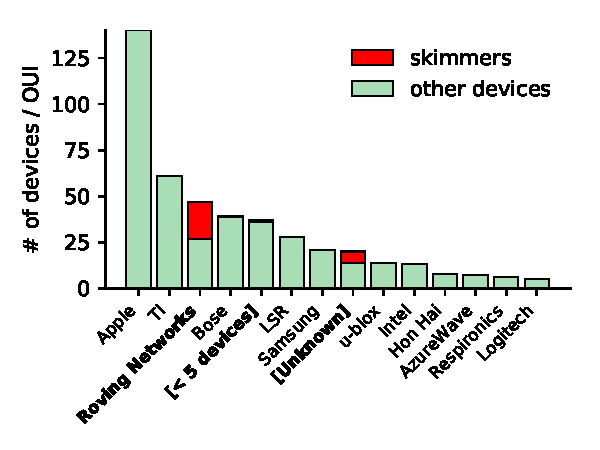
\includegraphics[width=\linewidth]{plots/all_hist_device_OUI.pdf}
%\caption{
%\label{fig:hist_device_OUI}
%Distribution of manufacturers per gas station visit. Skimmers are common amongst Roving Networks and unassigned
%manufacturers, and also occasionally smaller module producers.
%}
%\end{figure}

Within the set of Uncategorized devices, we next investigate their MAC prefixes
to see if the modules used in skimmers are also used in other devices.
%
%It is possible to identify many skimmers by looking at the MAC address of the
%discovered device and checking it against a hit-list of known skimmer module
%manufacturers.
%
%This hit-list is sourced from reports from law enforcement and previously
%discovered skimmers
%
This is an important observation because Scaife et al. found that a popular
detection application, SkimPlus~\cite{skimplus}, only considers on the MAC
prefix~\cite{scaifeoakland}.
%
Figure~\ref{fig:hist_device_OUI} shows the distribution of Unclassified device
MAC prefixes observed by Bluetana at gas stations (listed by manufacturer).

\begin{figure}
\centering
\includegraphics[width=\linewidth]{plots/uncat_hist_device_OUI.pdf}
\caption{
\label{fig:hist_device_OUI}
Many other devices appear to be using the same Bluetooth modules as skimmers.
}
\end{figure}

More than half of the RN modules seen at gas stations were in skimmers, but
there were many other devices that had RN modules as well.
%
However, the devices observed with MAC prefixes that are in the
\texttt{YY:YY:MM:DD} format (likely HC modules) were predominately skimmers.
%
The HC-based skimmer Bluetana detected with a known MAC prefix is not commonly
found at gas stations (not shown in figure).
%
The skimmer with the unknown MAC prefix that was not in date format is
difficult to detect with only MAC prefix, because Unknown MAC prefixes
were commonly found at gas stations.

Overall, \numberBTMACCoDfiltered~devices out of
\numberbtuncategorized~Uncategorized devices matched the MAC prefixes of
Bluetana-observed skimmers.
%Of the devices that had the same MAC prefix as observed skimmers, only
%\numberBTMACCoDfiltered~devices matched these MAC prefixes (out of
%\numberbtuncategorized~Uncategorized devices).
%
This reduces the number of stations where there could be skimmers to
\visitedstationsMACCoDfiltered~out of the~\totaluncatstation~stations that had Uncategorized devices.

%
%It was discovered that this MAC address was questionable after another HC-05
%module close in MAC range had been discovered by investigators.
%
%The device also had a distinctive name which allowed it to be flagged
%independently of OUI.
%
%There were also other devices with MAC prefixes not matching known IEEE assignments, that were not skimmers.
%
%For one of these skimmers, it was clear that the MAC was either purposefully
%misconfigured by the criminal or by the manufacturer of the module.
%
%For all HC-05 modules but two, the MAC addresses were simply the date of
%manufacture in the YY:YY:MM:DD format mentioned earlier.

\if 0 %what is this?
Collaborating with law
enforcement, we were able to develop a hit-list consisting of X addresses. In
fat, there was a case under which we found new manufacturers of skimmers, and
were able to use this new information to isolate skimmers we had seen 7 months
prior. The most common devices that we saw which were of the uncategorized
device class actually ended up being phones; we did not find any skimmers
masquerading as phones. We did see devices with no registered manufacturer. Some
of these were simply odd devices, others were skimmers.
\fi
%}}}

\subsubsection*{Default- and custom-named modules are often skimmers} %{{{

Finally, we investigate if skimmers can be differentiated from other devices by
their Device Name.
%
The remaining~\numberBTMACCoDfiltered~devices are Uncategorized, and their MAC prefixes are either: RN, \texttt{YY:YY:MM:DD}, Unknown, or seen on less than five devices.
%
Only
\totalskimmersfirstvisit~of these devices were confirmed to be
skimmers.\footnote{We do not include 22 of the Bluetana-detected skimmers in
this analysis because they were not detected on the first visit to a gas
station.}
%
In Figure~\ref{fig:hist_device_name}, we divide the remaining devices by their
category of Device Name, including: \emph{unnamed}, manufacturer
\emph{default}, known legitimate \emph{product}, and \emph{customized}.
%
Devices observed by Bluetana with default names are often skimmers.
%
Custom named devices were uncommonly found at gas stations, but often they are
skimmers.
%
Three skimmers were disguised as products, however all three were
distinguishable because their names were popular smartphones, which should not
have the MAC prefix of Bluetooth-to-Serial modules.
%
Bluetana missed capturing the Device Name for many of the skimmers, as well as other
devices that it detected.
%
 
%The relative portion of skimmers each category of  are 22.4\% for Unnamed,
%85.7\% for default, 6.9\% for product, and 33.3\% for custom.
%


\begin{figure}
    \centering
    \includegraphics[width=\linewidth]{plots/uncat_visit_hist_device_name.pdf}
    \caption{
    \label{fig:hist_device_name}
    Default and custom names distinguish skimmers from legitimate devices.
    }
\end{figure}


%

%We have seen skimmers disguise their names as cell phones in 3 of our 37 detection cases, and as generic non-malicious
%entities in 4 other cases.
%
%However, as the criminals are not also modifying the OUI of the devices to match, this can actually be used as a clear
%flag that a given device is a skimmer, i.e. seeing a roving networks module advertising itself as a Bluetooth speaker.

%\subsubsection*{Summary}

%In summary, we 

%\todo{We are likely not missing skimmers}

%}}}

%}}}

\subsection{Accuracy of Bluetooth-based Detection} %{{{

To evaluate the accuracy of Bluetooth-based detection, we analyze Bluetana scan
data collected during inspections in Arizona. Specifically, there was a 7-month
time period in which Bluetana was used by many of the Arizona inspectors
(October 7, 2018 -- May 7, 2019), and we compare the reports filed during these
inspections with the scan data that Bluetana collected.

\subsubsection*{Missed skimmers}
\label{sec:falsenegative}

%o measure the accuracy of Bluetooth 

During this time period, there were 27 inspections where
skimmers were found while an inspector was running Bluetana.
%
A total of 42 skimmers were
recovered during these inspections, of which Bluetana was able to detect 36.
%
Therefore, Bluetana missed detecting 14.3\% of the total skimmers recovered during these inspections.

We do not know exactly why Bluetooth-based scanning missed these skimmers.
%
Half of the missed skimmers were from inspections where Bluetana detected other
skimmers at the gas station.
%
It is likely that these missed skimmers were not powered on due to
improper installation.
%
The remaining missing skimmers may have been built with alternate
exfiltration methods, such as SMS~\cite{scaifeoakland}, or even physical
recovery~\cite{skimreaper2018}.

%Unfortunately, we were unable to test these skimmers in our lab because they
%were sent out to law enforcement immediately for further investigation.
%
	

\subsubsection*{Incorrectly detected skimmers}
\label{sec:falsepositive}

Bluetana highlighted a device in red during 45 Arizona inspections where no
skimmer was found.
%
There were 757 total inspections where inspectors used
Bluetana\footnote{This includes both routine and complaint/prior knowledge
triggered inspections},  Bluetana may have incorrectly detect skimmers in 5.9\%
of inspections.

%Considering Bluetana uses at least MAC prefix and Class-of-Device for
%highlighting, it is likely that these incorrectly classified 

Incorrectly identifying skimmers is likely due to the fact that  RN and HC
modules are used in a variety of legitimate products, some of which are seen in
and around gas stations.
%
We found RN and HC modules in radar-based speed limit signs, weather
sensors~\cite{rnbtweathersensor} automotive diagnostic scanners,
scales~\cite{rnbtscale} and fleet tracking systems~\cite{rnbteletrac}.
%
Some of these devices have Device Names that clearly indicate what product they
are (e.g., \texttt{}), but would be confused with skimmers if the Device Name
is missing.
%
Unfortunately, several of these products also use the default Device Names on
their Bluetooth modules (\emph{RNBT-xxxx} or \emph{HC-05}).
%
These legitimate devices will look exactly like skimmers.
%
Inspectors will need to rely on RSSI localization to determine if these devices
are located inside a gas pump.
%}}}

\if 0 % extra text{{{
\subsection{Skimmer Detection Likelihood}
This analysis shows skimmers constitute X number of the visited gas station.

Names:

custom - this many stations (\%)
default - this many stations (\%)
unnamed - this many stations (\%)

The extent to which this characterization will hold true in the coming years, or the extent to which criminals are
developing mechanisms to ``mask'' the fingerprint of their devices is unknown.
%
We include an extended discussion of these factors in section~\ref{sec:discussion}.

Bluetooth detection has additional benefits.
%
In most of the cases in which our application detected anomalous devices, it was able to alert inspectors to skimmers
in pumps which they were not planning upon opening and inspecting.
%
This includes two cases under which the inspectors were simply ``driving by'' a gas station.
%
For five of the skimmers well hidden inside of their pumps, our application was able to determine with confidence
that a skimmer was in the pump despite an initial failed visual inspection.



Additionally, the following discussion does not use Bluetooth Low Energy (BLE) or SDP fingerprinting as detection
mechanisms.
%
BLE introduces complications to potential skimmer discovery which are outside of the scope of this paper.
%
While BLE skimmers have been found in countries outside of the United States, law enforcement in the six states we have
surveyed have not yet come in contact with a device using the protocol.
%
For more details, see section\ref{sec:ble}.
%
Similarly, SDP introduces complications and additional hardware costs which are addressed in section\ref{sec:SDP}.


%\begin{center}
%    \begin{tabular}{r|c|c|c}
%        \textbf{Module} & \textbf{Vendor} & Chip-set & \textbf{Range} \\ \hline
%        RN-\{41/42\} & Roving Networks & CSR 417 & 100m/30m \\ HC-\{05/06\} &
%        \textit{Various} & CSR 417 & 30m \\
%    \end{tabular}
%\end{center}
%
%
%Both modules reported several factory-default fields that uniquely identify
%them, specifically their manufacturer (MAC prefix known as IEEE OID) is a valid
%OID for the manufacturer (Roving Networks). For the HC device which is
%inexpensive, a squatted MAC OID that has not yet been assigned to a manufacturer
%by IEEE. Also, the modules have default Bluetooth names that indicate which
%module they are, and a default device class (i.e., None)---most products have a
%name and device class that reflects the product (e.g., name: ``Bose
%Quiet-Comfort'', class: ``Headphones'').
%%
%Criminals may stick with the default configuration, even though every one of
%these fields can be changed with some hacking (see
%Section~\ref{sec:discussion:hiding}) values because it makes something look
%innocuous.
%
%In summary, the Bluetooth modules commonly found in skimmers may be identifiable
%in Bluetooth scans.
%%
%However, all of the parameters are configurable, and to confirm this hypothesis
%we will need to study skimmers in the wild.
%%
%Designing an Android app to collect this will allow us to study a large number
%of gas stations and collect data on the Bluetooth environment.
%%
%This crowd sourced deployment will allow us to determine if skimmers can be
%reliably detected with Bluetooth inquiry scanning alone.



%\section{Implementation and Overview of Findings}
%
%
%
%To conclude this section, we will give an overview of the effectiveness of
%finding skimmers using the information above.
%
%From the recorded inquiry response data of 115,199 devices and 29,818 unique
%devices near gas stations, we were able to isolate \todo{X} skimmers.
%%
%The primary method used to isolate questionable devices was MAC address
%filtering based upon OUI.
%%
%This method paired with geo-location filtering alone is able to reduce the number
%of potential devices down to 677, at the cost of a potentially high
%false-negative and false-positive rate.
%%
%Not only did this method fail to find two skimmers who OUI's were not in the
%``hit-list'' initially \noteby{MB}{and maybe even more!}, it also flagged a lot
%of non-skimmers which were found to be above suspicion after a manual analysis
%of the other features listed above.

%The prior overview demonstrates the efficacy of combining multiple pieces of scan
%data when finding skimmers.
%%
%In the rest of the paper, we will examine our dataset and discuss the individual
%benefits and drawbacks of each feature listed above.
%%
%From this, we will develop an understanding of how the components work together
%and filter out the noise of the typical gas station environment and detect
%skimmers.

%\todo{NOW THE BELOW IS A SECTION}
%\begin{figure}
%    \centering
%    \includegraphics[width=\linewidth]{plots/cdf_num_devices_seen.pdf}
%    \caption{
%    \label{fig:cdf_num_devices_seen}
%    Distribution of the number of classic and low energy Bluetooth devices seen
%    in a visit to a gas station. Classic devices are far less common than
%    low energy devices.
%    }
%\end{figure}

%We are focusing this discussion only on devices that are Classic Bluetooth,
%because all modules used by recovered skimmers are classic Bluetooth.
%%
%In Section~\ref{sec:ble}, we will describe how Bluetooth Low Energy-based
%skimmers will complicate detection via Bluetooth Scanning.

%\subsection{Collection and Hunt Summary}

%

%\subsection{The Anatomy of a Skimmer Fingerprint}
%
%In this section we will concretize skimmer anatomy based upon those database records which we have confirmed to be
%skimmers and the criminal evidence to which we were given physical access.
%%
%
%Foremost, our understanding of Skimmer anatomy revealed itself in two stages.
%%
%During the initial phase of research, we manually examined each record of our dataset, with a goal of finding the
%offending devices directly.
%%
%Over time, this methodology was refined and automated, and a more sophisticated set of features was analyzed.
%%
%Cases under which this was the case are mentioned explicitly.
%%
%Our interest lies within \textit{characteristics which make skimmers visible, characteristics which help
%skimmers to blend in, and characteristics which criminals could mask}.
%
%The motivating question is: ``can an automated application for skimmer detection be developed?''
%%
%From the following analysis, it should be clear that the answer is affirmative.
%
%\noteby{MB}{Now we look at our pile of skimmers. What is the distribution of MAC addresses, the distribution of
%names, the distribution of skimmers to gas stations, discuss how we were able to localize skimmers in every case in
%which we saw them (report the average minimum RSSI value, [and ideally its distance from the pump but I guess not?]!)
%talk about all the features that are bolded above. Here's some start text.}
%
%Law enforcement have informed us that the two common Bluetooth modules found in
%skimmers are:
%
%\begin{center}
%    \begin{tabular}{r|c|c|c}
%        \textbf{Module} & \textbf{Vendor} & Chip-set & \textbf{Range} \\ \hline
%        RN-\{41/42\} & Roving Networks & CSR 417 & 100m/30m \\ HC-\{05/06\} &
%        \textit{Various} & CSR 417 & 30m \\
%    \end{tabular}
%\end{center}
%
%
%Both modules reported several factory-default fields that uniquely identify
%them, specifically their manufacturer (MAC prefix known as IEEE OID) is a valid
%OID for the manufacturer (Roving Networks). For the HC device which is
%inexpensive, a squatted MAC OID that has not yet been assigned to a manufacturer
%by IEEE. Also, the modules have default Bluetooth names that indicate which
%module they are, and a default device class (i.e., None)---most products have a
%name and device class that reflects the product (e.g., name: ``Bose
%Quiet-Comfort'', class: ``Headphones'').
%%
%Criminals may stick with the default configuration, even though every one of
%these fields can be changed with some hacking (see
%Section~\ref{sec:discussion:hiding}) values because it makes something look
%innocuous.
%
%In summary, the Bluetooth modules commonly found in skimmers may be identifiable
%in Bluetooth scans.
%%
%However, all of the parameters are configurable, and to confirm this hypothesis
%we will need to study skimmers in the wild.
%%
%Designing an Android app to collect this will allow us to study a large number
%of gas stations and collect data on the Bluetooth environment.
%%
%This crowd sourced deployment will allow us to determine if skimmers can be
%reliably detected with Bluetooth inquiry scanning alone.

%\subsection{Feature Analysis}
%
%\subsubsection{Class of Device}
%
%
%\subsubsection{MAC address}


%\subsubsection{Geo-location and Received Signal Strength Indication (RSSI)}
%
%\subsubsection{Persistence} Many of the devices seen during the typical visit are transient, i.e. located in cars
%passing by and at the gas station for only a temporary amount of time; by accumulating records and only recording
%devices for which we receive multiple responses, we can also ensure that we are only selecting devices which are
%persistent at the gas station.
%\noteby{MB}{While we saw an average of X devices per gas station, X of these devices were non persistent, meaning we
%only got one response during the greater-than-a-minute time frame during which we were at the station. Amongst our
%skimmer devices, we got an average of X responses from the skimmer during the visits. This number is inflated by the
%possibility that seeing a skimmer \textit{causes} the investigator to scan more, however, out of the stations at
%which we did not see a skimmer, we saw an average of X persistent devices, indicating that the numbers of responses
%attained from skimmers are in line with the numbers typically seen from persistent devices.}

\subsubsection{Name}

%\todo{Move this section to Discussion}
%\subsubsection{Service Discovery Protocol} Bluetooth also provides the ability to
%query the services that a device can provide without establishing a connection
%to the device, the Service Discovery Protocol (SDP).
%%
%However, as of Android 6.0 the \texttt{BluetoothDevice} method
%\texttt{fetchUuidsWithSdp} will automatically trigger a pairing process with the
%device, making skimmer fingerprinting via SDP infeasible.

\todo{Move the rest of this section and integrate it into the analysis section
with the feature analysis}

The Bluetooth pairing process is most likely familiar due to its prevalence in
consumer electronics. Delving into greater technical detail, however, it follows
the following sequence.

The process begins with a stage called inquiry; this is the primary discovery
stage for Bluetooth enabled worker devices by a master device. The process is
set up in a specific manner to reduce conflict between device scanning, and
speed up discovery so that piconets with a master-worker dynamic can be quickly
set up. In inquiry cycles where the master device is not looking to connect to
devices for a specific purpose or service, the master device, known as the
inquirer, hops among 32 of Bluetooth's 79 1 MHz frequency channels, according to
a pseudo-random pattern seeded by a General Inquiry Access Code (GAIC) defined
within the standard. On each frequency, the device sends out an initial inquiry
packet consisting of the GAIC, a 28-bit CLK for synchronization purposes, and a
unique 48 bit address corresponding to the master device. 625 microseconds after
sending a packet on frequency $x$, the master device will listen on frequency $(x
+ 32) mod 79$ for a response from a possible listening device. Meanwhile, the
listening devices, known as scanners, will listen given frequencies in 1.28
second ``scan windows'', before hopping frequency in a predetermined manner in
order to account for the pseudo-random hopping of the inquirer device. Upon
recieval of the initial inquiry packet from the inquirer device, the scanner
device will begin a back-off based upon a uniformly distributed number of scan
slots between 0 and 1,023, meaning between 0 and (roughly) 640 ms. Once it
returns from this back-off state, the scanner device will begin scanning again,
and wait for a second inquiry packet from the master device. Once this is
received, the device will send out a Frequency Hopping Synchronization (FHS)
packet, in which the inquirer will learn the critical details of the device,
such as unique address. At this point, the inquirer device will finish its
inquiry process, followed by an initiation of paging with the worker device. It
is during this initial paging process that the Bluetooth device name and other
details will be exchanged. But notably, device discovery itself takes around
10.24 seconds in official measurements, and only 5.12 seconds to discover 99\%
of devices, according to more advanced analysis detailed in [Peterson,
Baldwin...].

In order to perform the Bluetooth device discovery detailed within our studies
of gas station environments, we used the Android operating system's
BluetoothAdapter interface to operating system services. A BluetoothAdapter
device discovery cycle typically consists of 12 seconds of inquiry scanning
followed by paging of those devices discovered in order to record device names
and details. There is a tradeoff present within following the default scan
interval; while allowing inquiry to complete ensures that various environmental
factors do not interfere with discovery and information is not lost, in a
crowd-sourced application where localization is a primary concern (in the case
of skimmers, ensuring that the device observed is within a pump), a larger
number of data-points for any given device is of larger concern. Thus, we offered
participants a variable setting for sane defaults between a 5 second scan and
the android default scan time. By restricting the inquiry period to five
seconds, more data-points were retrieved for each device. Additionally, because
paging is handled separately by the system service, this still allowed us to
retrieve device names. It is possible that this led us to miss out on the
discovery of some devices, and eager inquiry scanning to increase the amount of
localization points did interfere with paging, however, it roughly doubled the
number of geo-location points for each observed for each device, allowing for a
more fine-grained discovery of skimmers via the concentric ring based techniques
discussed in a later section. 

\subsubsection*{RSSI is detectably higher in the pump area of the station}

\begin{figure}
\centering
\includegraphics[width=\linewidth]{fig/rssi_motivation.pdf}
\caption{
\label{fig:rssi}
  Combining RSSI data with satellite imagery reveals if a device is located in the pump area of a gas station.
}
\end{figure}

When the skimmer responds to the Bluetooth scan request it responds with a
packet that contains the device's MAC address and class of device, and the
scanner uses the signal strength of this received packet to measure RSSI.
%
By the nature of being installed inside a gas pump, which is often a metal box,
the Bluetooth signal strength is typically only strong in the pump area.
%
Other devices that we suspected may be skimmers, all had a low signal strength
in the pump area, because aside from the cars parked at the pumps, the only
places where a Bluetooth device would be located in the pump area would be
inside the pump.
%
We show this by combining the RSSI with the geo-location from GPS, and satellite
imagery of the gas station, it becomes clear that the inside of a gas pump
(example shown in Figure~\ref{fig:rssi}).
%
While at a gas station this can be seen by moving toward the pump area to see
if the device's signal strength increases. 



\fi %}}}


%%!TEX root = paper_main.tex
\label{sec:appendix}
The appendix contains excerpts from various public court documents related to cases of credit card skimming. These excerpts provide anecdotal data about the monetary impact of the skimmer 
problem.

\section{Cashout Value}
\label{sec:appendix:cashout}

\subsection*{USA v. Hristov et al \cite{hristov}}
"\dots Bank of America suffered a loss of \$33,000 with 36
compromised customer accounts.  Citizens Bank suffered a loss of
\$91,580 with 74 compromised customer accounts \dots" 

\subsection*{USA v. Cristea et al \cite{cristea}}
"\dots Altogether, on February 21,2016, FBI surveillance observed Cristea, 
Co-conspirator \#1, and Co-conspirator \#2 go to approximately 12 
different locations, where, according to CardTronic's records, they
withdrew at least \$7,000 from at least 18 First National Bank accounts \dots" 

\subsection*{USA v. Khasanov et al \cite{mekhakian}}
"\dots USPS agents thereafter conducted record checks on the purchased USPS money orders
and discovered that 10 of the 57 money orders had been purchased with 5 payment numbers
issued by Citibank \dots"

\begin{center}
    \begin{tabular}{|c|c|c|}
    	\hline
        \textbf{Date} & \textbf{Location of USPS} & \textbf{Amount} \\ 
        \hline 
        Aug 4 2017 & Waldorf, MD & \$2,904.80 \\
        \hline
        Aug 7 2017 & Washington, DC & \$1,492.80 \\
        \hline
        Aug 7 2017 & McLean, VA & \$1,400.00 \\
        \hline
        Aug 7 2017 & Washington, DC & \$1,803.20 \\
        \hline
        Aug 7 2017 & Hyattsville, MD & \$792.05 \\
    	\hline
    \end{tabular}
\end{center}
 

\subsection*{USA v. Aqel \cite{aqel}}
"\dots the Probation Officer also notes that the actual loss to victims
was \$8,327.58. Id. Similarly, the Probation Officer notes that while Mr. Aqel possessed 120 stolen credit
card numbers, only 23 of those numbers were used to make purchases \dots" 

\subsection*{USA v. Rodriguez et al \cite{rodriguez}}
"\dots Between on or about July 7, 2016, and on or about July 20, 2016, Defendant ... attempted to conduct approximately 133 retail transactions totaling in excess of \$27,000 ... using approximately 90 counterfeit access devices re-encoded with credit/debit account information that were obtained by a skimming device placed on the point of sale terminal of a gas pump \dots " 

\subsection*{Application for Search Warrant, 2:18mj1277\cite{estrada}}
"\dots On April 14, 2016, a man (later identified as Estrada) used a fraudulent Visa credit card and a fraudulent MasterCard to purchase two \$300.00 gift cards from the Kohl's store \dots"

\subsection*{USA v. Konstantinov et al \cite{alisuretove}}
"\dots In total, the defendants compromised approximately 524 debit card accounts and made approximately 779 fraudulent withdrawals, totaling \$348,376.80 \dots"

\begin{comment}
\subsection{Skimmer residence time}
\label{sec:appendix:residencetime}

\subsubsection*{USA v. Rodriguez et al \cite{rodriguez}}
"\dots On or about April 4, 2016, Defendant ... installed a skimmer device on the point of sale terminal inside a gas pump located at a Circle K Gas Station in Fairview Park ... skimmer device was discovered on the gas pump by an employee on or about April 15, 2016 \dots

\dots On or about April 17, 2016, unknown members of the conspiracy installed a skimmer device on the point of sale terminal inside a gas pump at the Circle K Gas Station \dots skimmer was discovered by employees on or about April 19, 2016 \dots"

\subsubsection*{Application for Search Warrant, 2:18mj704 \cite{conde}}
"\dots (Victim \#1) whose debit card had been compromised and used at a Home Depot in an attempt to purchase a gift card \dots Victim \#1 stated he had only used that card once, on June 10, 2018, at the same gas station and pump where the skimmer device was recovered on June 21, 2018 \dots" 
\end{comment}
\section{Credit/Debit cards per skimmer per day}
\label{sec:appendix:cardsperskimmer}

\subsection*{Application for Search Warrant, 2:18mj1277 \cite{estrada}}
"\dots On September 9, 2016, an employee at Jilly's Mobil \dots reported to Detective Craig Meyer that he had found what appeared to be a skimmer on pump \#8 \dots Detective Meyer downloaded and exported the data stored on the skimmer taken from Jilly's Mobil pump \#8. The results showed data for 221 victim credit card accounts \dots

\dots Detective Meyer reviewed the video surveillance footage for Jilly's Mobil from September 1, 2016. At 1:38 PM on September 1st, a red Ford Explorer drove to pump 8. The Ford Explorer was positioned in a manner whereby the opened passenger door blocked the view of the gas pump by the store employee inside the Jilly's Mobil \dots"





\chapter{BLE Physical-Layer tracking of Mobile devices}
%%!TEX root = paper.tex
%%% datadef.tex - Macros for various results used in tables and text.

\newcommand\pctmatchskimmer{3.98\%} % Percentage of classic bluetooth devices seen at gas stations that match the profile of skimmers

\newcommand\visitedgasstations{1,185} %Total number of gas stations visited in our study
%\newcommand\inspectedgasstationsAZ{757} %Total number of inspections by bluetana
\newcommand\inspectedgasstationsAZ{757} %Total number of gas stations visited in AZ in our study
\newcommand\visitedgasstationsAZ{491} %Total number of gas stations visited in AZ in our study
\newcommand\totaluncatstation{143} % Total number of gas stations where uncategorized BT devices were seen
\newcommand\visitedstationsMACCoDfiltered{79} % Number of gas stations visited where BT devices matching suspicious MAC + CoD were seen

\newcommand\totalskimmersBluetana{33}
\newcommand\Bluetanafraudprevented{\$495,000} % Total monetary fraud prevented by Bluetana assuming skimmers operated for one day. Will be the product of totalskimmersBluetana X 15,000

\newcommand\totalskimmers{64} %Total skimmers found in the field in our study
\newcommand\totalskimmersLE{23} %Total skimmers given to us by LE
\newcommand\totalskimmersseen{87} %Total skimmers ever detected by Bluetana. This is sum of found in field + obtained from LE
\newcommand\averageclassicBTperstation{2.2} %Average classic BT devices seen per gas station
\newcommand\stdevclassicBTperstation{2.05} % Std deviation of classic BT devices seen per gas station


%Following two macros are AZ specific and can be merged if we go through with AZ analysis
\newcommand\azskiminspect{7,325} %Total skimmer inspections done in Arizona 2016-2018.
\newcommand\azpercentskimfound{1.5\%} %Percentage of inspections Arizona 2016-2018 in which skimmers were found 
%%%%%%%%%%%%%%%%%%%


\newcommand\totalbtobserved{2,214} %Total number of BT devices observed across all visited gas stations
\newcommand\percentbtuncategorized{8.4\%} % Percent of total BT devices at visited gas stations that had uncategorized BT CoD
\newcommand\numberbtuncategorized{187} % Number of total BT devices at visited gas stations that had uncategorized BT CoD
\newcommand\numberBTMACCoDfiltered{102} % Number of total BT devices at visited gas stations that had suspect MAC + CoD
\newcommand\totalskimmersfirstvisit{42} % Total skimmers that were found in the visit to gas station (not including those found during a second visit to the gas station)


\newcommand\numvolunteers{44} %Total number of data collectors we had across US
\newcommand\skimmerfraudXVIIIUSA{\$17.43 million} % Total potential fraud in one day of operation of skimmers installed across SD,AZ,FL in 2018. Will be product of skimmers recovered X 15000

\newcommand\Bluetanaskimmerfield{33} %Skimmers found in the field without us 4 involved (Basically all of AZ, SDWM,LVPD)

\newcommand\Bluetanaskimstations{34} % Number of gas stations in which Bluetana saw a skimmer and it was recovered, US-wide

\newcommand\skimmeroneminutepercent{80\%} %Percent fraction of skimmers detected within one minute of arriving at a gas station

\newcommand\skimmerdetectiontimemedian{3} %Median time in seconds after entering 150 ft of gas station, when Bluetana can detect a skimmer 
\newcommand\skimmerdetectiontimemean{33} %mean time in seconds after entering 150 ft of gas station, when Bluetana can detect a skimmer 
\newcommand\skimmerdetectiontimestd{60} %mean time in seconds after entering 150 ft of gas station, when Bluetana can detect a skimmer 

%\newcommand\usssfyXVIIIincidents{13}
%\newcommand\usssfyXVIIIsksta{11}
%\newcommand\usssfyXVIIIstarisk{1.26\%}
%\newcommand\usssfyXVIIIrptsksta{2}
%\newcommand\usssfyXVIIIskimmers{42}
%\newcommand\usssfyXVIIIskperinc{3.2}
%
\newcommand\sdfyXVIIIskimmers{42}
\newcommand\azXVIskimmers{88}
\newcommand\azXVIIskimmers{57}
\newcommand\azXVIIIskimmers{148}
\newcommand\azALLskimmers{293}
\newcommand\flXVIskimmers{207}
\newcommand\flXVIIskimmers{650}
\newcommand\flXVIIIskimmers{972}
\newcommand\flALLskimmers{1,829}

\newcommand\sdfyXVIIIsksta{11}
\newcommand\azXVIsksta{54}
\newcommand\azXVIIsksta{46}
\newcommand\azXVIIIsksta{86}
\newcommand\azALLsksta{134}
\newcommand\flXVIsksta{162}
\newcommand\flXVIIsksta{432}
\newcommand\flXVIIIsksta{524}
\newcommand\flALLsksta{1,029}

\newcommand\sdfyXVIIIskperinc{3.2}
\newcommand\azXVIskperinc{1.6}
\newcommand\azXVIIskperinc{1.2}
\newcommand\azXVIIIskperinc{1.7}
\newcommand\azALLskperinc{2.2}
\newcommand\flXVIskperinc{1.3}
\newcommand\flXVIIskperinc{1.5}
\newcommand\flXVIIIskperinc{1.8}
\newcommand\flALLskperinc{1.7}

\newcommand\sdfyXVIIIskpercap{11.9} % 42 / (3.338m + 183k)
\newcommand\azXVIskpercap{4.3} % 88 / (20.66m)
\newcommand\azXVIIskpercap{2.7} % 57 / (20.98m)
\newcommand\azXVIIIskpercap{6.9} % 148 / (21.31m)
\newcommand\azALLskpercap{14.0} % 293 / (20.98m)
\newcommand\flXVIskpercap{10.0} % 207 /20.6m
\newcommand\flXVIIskpercap{31.1} % 650 / 20.9m
\newcommand\flXVIIIskpercap{45.6} % 972 / 21.3m
\newcommand\flALLskpercap{87.4} % 1829 / 20.93

\newcommand\fyXVIIIstart{October 1, 2017}
\newcommand\fyXVIIIend{September 30, 2018}

%\newcommand\azALLinspects{6,828}
%%\newcommand\azALLinspects{\smaller[3]\bfseries${}^{\texttt{{\textbackslash}azALL}}_{\texttt{\phantom{\textbackslash}inspects}}$}
%\newcommand\azXVIinspects{2,447}
%%\newcommand\azXVIinspects{\smaller[3]\bfseries${}^{\texttt{{\textbackslash}azXVI}}_{\texttt{\phantom{\textbackslash}inspects}}$}
%\newcommand\azXVIIinspects{1,857}
%%\newcommand\azXVIIinspects{\smaller[3]\bfseries${}^{\texttt{{\textbackslash}azXVII}}_{\texttt{\phantom{\textbackslash}inspects}}$}
%\newcommand\azXVIIIinspects{2,524}
%%\newcommand\azXVIIIinspects{\smaller[3]\bfseries${}^{\texttt{{\textbackslash}azXVIII}}_{\texttt{\phantom{\textbackslash}inspects}}$}
%
%\newcommand\azALLskinsp{2,894}
%%\newcommand\azALLskinsp{\smaller[3]\bfseries${}^{\texttt{{\textbackslash}azALL}}_{\texttt{\phantom{\textbackslash}skinsp}}$}
%\newcommand\azXVIskinsp{939}
%%\newcommand\azXVIskinsp{\smaller[3]\bfseries${}^{\texttt{{\textbackslash}azXVI}}_{\texttt{\phantom{\textbackslash}skinsp}}$}
%\newcommand\azXVIIskinsp{753}
%%\newcommand\azXVIIskinsp{\smaller[3]\bfseries${}^{\texttt{{\textbackslash}azXVII}}_{\texttt{\phantom{\textbackslash}skinsp}}$}
%\newcommand\azXVIIIskinsp{1,202}
%%\newcommand\azXVIIIskinsp{\smaller[3]\bfseries${}^{\texttt{{\textbackslash}azXVIII}}_{\texttt{\phantom{\textbackslash}skinsp}}$}
%
%\newcommand\azALLreginsp{3,934}
%%\newcommand\azALLreginsp{\smaller[3]\bfseries${}^{\texttt{{\textbackslash}azALL}}_{\texttt{\phantom{\textbackslash}reginsp}}$}
%\newcommand\azXVIreginsp{1,508}
%%\newcommand\azXVIreginsp{\smaller[3]\bfseries${}^{\texttt{{\textbackslash}azXVI}}_{\texttt{\phantom{\textbackslash}reginsp}}$}
%\newcommand\azXVIIreginsp{1,104}
%%\newcommand\azXVIIreginsp{\smaller[3]\bfseries${}^{\texttt{{\textbackslash}azXVII}}_{\texttt{\phantom{\textbackslash}reginsp}}$}
%\newcommand\azXVIIIreginsp{1,322}
%%\newcommand\azXVIIIreginsp{\smaller[3]\bfseries${}^{\texttt{{\textbackslash}azXVIII}}_{\texttt{\phantom{\textbackslash}reginsp}}$}
%
%\newcommand\azALLskinsppct{42.4\%} % 2894/6828
%%\newcommand\azALLskinsppct{\smaller[3]\bfseries${}^{\texttt{{\textbackslash}azALL}}_{\texttt{\phantom{\textbackslash}skinsppct}}$}
%\newcommand\azXVIskinsppct{49.4\%} % 939/2447
%%\newcommand\azXVIskinsppct{\smaller[3]\bfseries${}^{\texttt{{\textbackslash}azXVI}}_{\texttt{\phantom{\textbackslash}skinsppct}}$}
%%\newcommand\azXVIIskinsppct{}
%\newcommand\azXVIIskinsppct{40.4\%}
%%\newcommand\azXVIIIskinsppct{}
%\newcommand\azXVIIIskinsppct{36.9\%}
%
%%\newcommand\azALLreginsppct{}
%\newcommand\azALLreginsppct{57.6\%}
%%\newcommand\azXVIreginsppct{}
%\newcommand\azXVIreginsppct{50.6\%}
%%\newcommand\azXVIIreginsppct{}
%\newcommand\azXVIIreginsppct{59.6\%}
%%\newcommand\azXVIIIreginsppct{}
%\newcommand\azXVIIIreginsppct{63.1\%}
%
%%\newcommand\azALLincidents{}
%\newcommand\azALLincidents{232}
%%\newcommand\azXVIincidents{}
%\newcommand\azXVIincidents{61}
%%\newcommand\azXVIIincidents{}
%\newcommand\azXVIIincidents{54}
%%\newcommand\azXVIIIincidents{}
%\newcommand\azXVIIIincidents{117}
%
%%\newcommand\azALLskinc{}
%\newcommand\azALLskinc{7.3\%}
%%\newcommand\azXVIskinc{}
%\newcommand\azXVIskinc{3.3\%}
%%\newcommand\azXVIIskinc{}
%\newcommand\azXVIIskinc{5.5\%}
%%\newcommand\azXVIIIskinc{}
%\newcommand\azXVIIIskinc{10.2\%}
%
%%\newcommand\azALLreginc{}
%\newcommand\azALLreginc{92.7\%}
%%\newcommand\azXVIreginc{}
%\newcommand\azXVIreginc{96.7\%}
%%\newcommand\azXVIIreginc{}
%\newcommand\azXVIIreginc{94.5\%}
%%\newcommand\azXVIIIreginc{}
%\newcommand\azXVIIIreginc{89.8\%}
%
%%\newcommand\azALLinsphr{}
%\newcommand\azALLinsphr{8.0\%}
%%\newcommand\azXVIinsphr{}
%\newcommand\azXVIinsphr{5.1\%}
%%\newcommand\azXVIIinsphr{}
%\newcommand\azXVIIinsphr{7.2\%}
%%\newcommand\azXVIIIinsphr{}
%\newcommand\azXVIIIinsphr{12.5\%}
%
%%\newcommand\azALLskinsphr{}
%\newcommand\azALLskinsphr{6.1\%}
%%\newcommand\azXVIskinsphr{}
%\newcommand\azXVIskinsphr{2.6\%}
%%\newcommand\azXVIIskinsphr{}
%\newcommand\azXVIIskinsphr{3.9\%}
%%\newcommand\azXVIIIskinsphr{}
%\newcommand\azXVIIIskinsphr{9.1\%}
%
%%\newcommand\azALLreginsphr{}
%\newcommand\azALLreginsphr{8.2\%}
%%\newcommand\azXVIreginsphr{}
%\newcommand\azXVIreginsphr{5.2\%}
%%\newcommand\azXVIIreginsphr{}
%\newcommand\azXVIIreginsphr{7.6\%}
%%\newcommand\azXVIIIreginsphr{}
%\newcommand\azXVIIIreginsphr{13.1\%}
%
%\newcommand\azXVIadvantage{49.2\%}
%\newcommand\azXVIIadvantage{37.1\%}
%\newcommand\azXVIIIadvantage{17.9\%}
%\newcommand\azALLadvantage{30.6\%}
%
%\newcommand\azXVIencoreIII{6.5\%}
%\newcommand\azXVIIencoreIII{14.7\%}
%\newcommand\azXVIIIencoreIII{24.8\%}
%\newcommand\azALLencoreIII{17.6\%}
%
%\newcommand\azXVIencoreV{34.4\%}
%\newcommand\azXVIIencoreV{7.4\%}
%\newcommand\azXVIIIencoreV{51.3\%}
%\newcommand\azALLencoreV{36.6\%}
%
%\newcommand\azXVIvista{3.4\%}
%\newcommand\azXVIIvista{3.7\%}
%\newcommand\azXVIIIvista{2.6\%}
%\newcommand\azALLvista{3.1\%}
%
%\newcommand\azXVIovation{6.5\%}
%\newcommand\azXVIIovation{37.1\%}
%\newcommand\azXVIIIovation{3.4\%}
%\newcommand\azALLovation{12.1\%}
%
%%\newcommand\azALLsksta{}
%\newcommand\azALLsksta{172}
%%\newcommand\azXVIsksta{}
%\newcommand\azXVIsksta{54}
%%\newcommand\azXVIIsksta{}
%\newcommand\azXVIIsksta{42}
%%\newcommand\azXVIIIsksta{}
%\newcommand\azXVIIIsksta{76}
%
%%\newcommand\azALLstarisk{}
%\newcommand\azALLstarisk{8.7\%}
%%\newcommand\azXVIstarisk{}
%\newcommand\azXVIstarisk{2.8\%}
%%\newcommand\azXVIIstarisk{}
%\newcommand\azXVIIstarisk{2.1\%}
%%\newcommand\azXVIIIstarisk{}
%\newcommand\azXVIIIstarisk{3.8\%}
%
%%\newcommand\azALLskimmers{}
%\newcommand\azALLskimmers{299}
%%\newcommand\azXVIskimmers{}
%\newcommand\azXVIskimmers{85}
%%\newcommand\azXVIIskimmers{}
%\newcommand\azXVIIskimmers{63}
%%\newcommand\azXVIIIskimmers{}
%\newcommand\azXVIIIskimmers{151}
%
%%\newcommand\azALLstreet{}
%\newcommand\azALLstreet{\smaller[3]\bfseries${}^{\texttt{{\textbackslash}azALL}}_{\texttt{\phantom{\textbackslash}street}}$}
%%\newcommand\azXVIstreet{}
%\newcommand\azXVIstreet{\smaller[3]\bfseries${}^{\texttt{{\textbackslash}azXVI}}_{\texttt{\phantom{\textbackslash}street}}$}
%%\newcommand\azXVIIstreet{}
%\newcommand\azXVIIstreet{\smaller[3]\bfseries${}^{\texttt{{\textbackslash}azXVII}}_{\texttt{\phantom{\textbackslash}street}}$}
%%\newcommand\azXVIIIstreet{}
%\newcommand\azXVIIIstreet{\smaller[3]\bfseries${}^{\texttt{{\textbackslash}azXVIII}}_{\texttt{\phantom{\textbackslash}street}}$}
%
%%\newcommand\azALLstore{}
%\newcommand\azALLstore{\smaller[3]\bfseries${}^{\texttt{{\textbackslash}azALL}}_{\texttt{\phantom{\textbackslash}store}}$}
%%\newcommand\azXVIstore{}
%\newcommand\azXVIstore{\smaller[3]\bfseries${}^{\texttt{{\textbackslash}azXVI}}_{\texttt{\phantom{\textbackslash}store}}$}
%%\newcommand\azXVIIstore{}
%\newcommand\azXVIIstore{\smaller[3]\bfseries${}^{\texttt{{\textbackslash}azXVII}}_{\texttt{\phantom{\textbackslash}store}}$}
%%\newcommand\azXVIIIstore{}
%\newcommand\azXVIIIstore{\smaller[3]\bfseries${}^{\texttt{{\textbackslash}azXVIII}}_{\texttt{\phantom{\textbackslash}store}}$}
%
%%\newcommand\azALLskperinc{}
%\newcommand\azALLskperinc{1.3}
%%\newcommand\azXVIskperinc{}
%\newcommand\azXVIskperinc{1.4}
%%\newcommand\azXVIIskperinc{}
%\newcommand\azXVIIskperinc{1.2}
%%\newcommand\azXVIIIskperinc{}
%\newcommand\azXVIIIskperinc{1.3}
%
%%\newcommand\azALLskperskinc{}
%\newcommand\azALLskperskinc{1.5}
%%\newcommand\azXVIskperskinc{}
%\newcommand\azXVIskperskinc{2.5}
%%\newcommand\azXVIIskperskinc{}
%\newcommand\azXVIIskperskinc{1.3}
%%\newcommand\azXVIIIskperskinc{}
%\newcommand\azXVIIIskperskinc{1.5}
%
%%\newcommand\azALLskperreginc{}
%\newcommand\azALLskperreginc{1.2}
%%\newcommand\azXVIskperreginc{}
%\newcommand\azXVIskperreginc{1.3}
%%\newcommand\azXVIIskperreginc{}
%\newcommand\azXVIIskperreginc{1.2}
%%\newcommand\azXVIIIskperreginc{}
%\newcommand\azXVIIIskperreginc{1.3}
%
%
%%\newcommand\azALL{}
%%\newcommand\azXVI{}
%%\newcommand\azXVII{}
%%\newcommand\azXVIII{}
%
%
%%%% TABLE usss-results
%% Note: FY18 encoded using Roman numerals as fyXVII.
%
%\newcommand\usssfyXVIIIstart{October 1, 2017}
%\newcommand\usssfyXVIIIend{September 30, 2018}
%\newcommand\usssfyXVIIIincidents{13}
%\newcommand\usssfyXVIIIsksta{11}
%\newcommand\usssfyXVIIIstarisk{1.26\%}
%\newcommand\usssfyXVIIIrptsksta{2}
%\newcommand\usssfyXVIIIskimmers{42}
%\newcommand\usssfyXVIIIskperinc{3.2}
%
%%%% TABLE skimcost
%
%

\section{Introduction}

The mobile devices we carry every day, such as smartphones and
smartwatches, increasingly function as wireless tracking
beacons. These devices continuously transmit short-range wireless
messages using the Bluetooth Low Energy (BLE) protocol.  These beacons
are used to indicate proximity to any passive receiver within range.
Popular examples of such beacons include the COVID-19 electronic
contact tracing provided on Apple and Google
Smartphones~\cite{9-millionca} as well as Apple's intrinsic Continuity
protocol, used for automated device hand-off and other proximity
features~\cite{applecontinuity}.

However, by their nature, BLE wireless tracking beacons have the
potential to introduce significant privacy risks. For example, an
adversary might stalk a user by placing BLE receivers near locations
they might visit and then record the presence of the user's
beacons~\cite{exposurefaqmanual,dp3t}.  To address these issues, common BLE proximity
applications cryptographically anonymize and periodically rotate the
identity of a mobile device in their beacons. For instance, BLE
devices periodically re-encrypt their MAC address, while still
allowing trusted devices to determine if these addresses match the
device's true MAC address~\cite{bluetoothprivacy}. Similarly, COVID-19 contact tracing
applications regularly rotate identifiers to ensure that receivers
cannot link beacons from the same device over time~\cite{exposurenotificationmanual}.

While these mechanisms can foreclose the use of beacon content as a
stable identifier, attackers can bypass these countermeasures by
fingerprinting the device at a lower layer. Specifically, prior work
has demonstrated that wireless transmitters have imperfections
introduced in manufacturing that produce a unique physical-layer
fingerprint for that device (e.g., Carrier Frequency Offset and I/Q
Offset). Physical-layer fingerprints can reliably differentiate many
kinds of wireless chipsets~\cite{rfidphysical_danev,Brik_radiometric,transientBT_Hall,suskitransient,tximperfections_polak,femtocell_kennedy,adsb,subgrfid}, including a recent attempt to
distinguish 10,000 WiFi~\cite{kaushik10000wifi} chipsets.

However, no prior work has evaluated the
practicality of such physical-layer identification attacks in a real-world
environment. 
%
Indeed, prior to BLE tracking beacons, no mobile device wireless
protocol transmitted frequently enough---especially when idle---to make
such an attack feasible. 
%
In contrast, today it is common to find tens and hundreds of personal devices transmitting these BLE beacons at all public locations -- office buildings, public library, coffee shops and others.
%
For an attacker, even with a precise fingerprint, locating one target device in such public locations is a needle in a haystack problem --- we don't know the limitations to uniquely differentiating one BLE device in this "noise" of several other BLE devices.
%

In this chapter, we take an empirical measurement approach to understanding the practicality of this tracking threat. 
%
We develop a technique to estimate high precision fingerprints from BLE beacons.
%
We then perform BLE beacon data collection in lab on devices that we control, and also uncontrolled data collection of BLE beacons from mobile devices seen at a variety of public locations.
%
Using our fingerprint technique, we analyze these beacons from real-world devices to understand the scope of this privacy threat, and how likely is an attacker at being successful in locating their target. 
%
In particular the contributions of our work are as below:

\begin{enumerate}
\item Using lab-bench experiments on BLE devices we own, we identify four primary challenges to identifying BLE devices in the field: (1) BLE devices have a variety of chipsets that have different
hardware implementations, (2) applications can configure the BLE transmit
power level, resulting in some devices having lower SNR BLE transmissions,
(3) the temperature range that mobile devices encounter in the field
can introduce significant changes to physical-layer impairments, and (4) the low-cost
receivers that an attacker can use in the wild for RF fingerprinting may be significantly less accurate than the tools used in prior studies~\cite{Brik_radiometric}.
 
\item We perform an empirical study through a set of field experiments to evaluate how
significantly these challenges diminish an attacker's ability to identify
mobile devices in the field. We leverage the fact that BLE tracking beacons are
already used on many mobile devices to perform an uncontrolled field study
where we evaluate the feasibility of tracking BLE devices when they
are operating in public spaces where there are hundreds of other nearby devices.
 To the best of our knowledge, our work is
the first to evaluate the feasibility of an RF fingerprinting attack in
real-world scenarios.
\end{enumerate}

Through these empirical studies, we show that even when there are hundreds of devices we encountered in the field, it is still feasible to uniquely identify 
a specific mobile device by its physical-layer fingerprint. 
%
However, we also
observe that certain devices have similar fingerprints to others, and temperature
variations can change a device's metrics. 
%
Both of these issues can lead to significant confusion in distinguishing mobile devices.
%
In summary, we find that physical layer tracking of
BLE devices is indeed feasible, but it is only
reliable under limited conditions, and for specific devices with extremely
unique fingerprints, and when the target device has a relatively stable
temperature. 


%!TEX root = paper_main.tex
\section{Background}

\label{sec:threatmodel}

In this section, we define the threat model for a tracking attack on a BLE based mobile device. 
%
Following that we provide details on how extensive the threat is by exploring how all popular personal mobile devices are continuously and frequently transmitting BLE beacons.

%In this section we describe the threat model of location privacy attacks on
%BLE-enabled mobile devices. Then, we demonstrate how location privacy attacks
%are a significant threat today because popular mobile devices 
%continuously, and frequently, transmit BLE advertisements.

%Then, we explain why it may be possible to defeat BLE's built in anonymization
%techniques by physical-layer identity in the transmissions, that can defeat
%BLE's built-in anonymization techniques.

\subsection{Threat model: Passive fingerprinting of BLE mobile devices}
%
We consider an attacker that intends to detect when the target -- a particular user possessing the target mobile device --- is at a specific location (e.g. a room in a building or a crowded public place).
%
The attacker must possess a software-defined radio (SDR) to capture the raw \iq data of the BLE beacons transmitted by nearby mobile devices.
%
Even though a lot of SDR tools are expensive, we show in Section~\ref{sec:hadi:sdr} that a modest hobbyist-level SDR ($\sim$\$150) is sufficient for the attacker.
%

The attacker first captures a fingerprint of their target's mobile device.
%
They do so by getting close to them and capturing BLE beacons from their mobile device.
%
Then they use these BLE beacons to estimate unique physical-layer properties of the BLE transmitter hardware, such as CFO and \iq offset -- these define the fingerprint of the target mobile device.
%

Armed with the fingerprint of their target, the attacker sets up the receiver at the eventual attack location where they want to track the target.
%
The attacker captures beacon packets from all mobile devices at the location, estimates the physical-layer properties and compares it to the target fingerprint.
%
If the fingerprint matches, the attacker knows that the target is at the location.
%
The more frequently the BLE device transmits, the more likely the attacker is
to receive a transmission if a user passes by.  Also, the more accurate the
fingerprinting technique is, the better the attacker can differentiate the
target from other nearby devices.
%

\subsection{Extent of threat: Popular mobile devices are vulnerable} %{{{

Increasingly,  mobile devices are adding BLE beacons to
provide new features.
%
Most notably, during the COVID-19 pandemic, governments have installed software
on iPhones and Android phones to send constant BLE advertisements for digital
contact tracing: devices listen for nearby transmissions to determine if and
for how long another device was nearby.
%
Also, Apple and Microsoft operating systems have recently added BLE beaconing
to their devices for two inter-device communication features: lost device
tracking, and seamless user switching between devices (e.g., Apple's Continuity
Protocol, Microsoft's Universal Windows
Platform)~\cite{Iphonetracking_becker}.
%
Therefore, BLE beacons are now common on many mobile platforms, including:
phones, laptops, and smartwatches. 
 
%BLE beaconing presents a significant location privacy threat for
%the following reasons:
 
%\subsubsection*{BLE beaconing is widely deployed on mobile devices.}
%
%When mobile devices are running these applications, they need to constantly
%transmit BLE advertisements.

Fingerprinting and tracking a BLE device requires the device to act like a
tracking beacon: it must transmit continuously and frequently.
%
%Continuous beaconing creates a significant threat where users' devices are
%constantly emitting a signal that may be able to uniquely identify them.
%
We observed the BLE behavior of popular devices to determine if they transmit
continuously, and how frequently they transmit if they do.
%
Specifically, we isolated six popular devices in a Faraday
cage---ensuring they were the source of the transmissions---and we used an SDR sniffer
to collect all BLE advertisements (i.e., BLE beacons) transmitted on any of the three advertising channels. 
%
We observed the following:

\begin{table}
    \centering\small
    %\begin{minipage}{\textwidth}
      \captionsetup{justification=centering}
      \caption{BLE beaconing behavior of popular mobile devices.}
    \begin{tabular}{llc}
    \toprule
    \colname{Product} & \colname{OS} & \colname{\# of adverts/minute} \\
    \midrule
    iPhone 10 & iOS & 872 \\
    Thinkpad X1 Carbon & Windows & 864 \\
    MacBook Pro 2016 & OSX & 576 \\
    %Fitbit Alta HR & 54 \\
    Apple Watch 4 & iOS & 598 \\
    Google Pixel 5$^{*}$ & Android & 510 \\
    Bose QC35 & Unknown & 77 \\
    \bottomrule
    \multicolumn{3}{l}{\footnotesize{$^{*}$Only beacons with COVID-19 contact tracing enabled.}}

\end{tabular}

\begin{comment}
\begin{tabular}{lcc}
    \toprule
    \colname{Product}  & \colname{\# of adverts/minute} & \colname{Device state during test}\\
    \midrule
    iPhone 10 & 872 & Screen off and locked\\
    MacBook Pro 2016 & 576 & Screen off, \\
    Thinkpad X1 Carbon & 864 & Screen off, laptop on battery\\
    Fitbit Alta HR & 54 \\
    Apple Watch 4 & 598 \\
    Bose QC35 & 77 \\
    \bottomrule

\end{tabular}
\end{comment}

    
    \label{tab:beacon_rate}
    %\end{minipage}
\end{table}

\begin{enumerate}
\item \textbf{Mobile devices send BLE beacons continuously: }
%
We observed continuous BLE beaconing from all the six mobile devices shown in Table~\ref{tab:beacon_rate}.
%
%Mobile devices that transmit BLE beacons do so continuously, regardless
%of the user's activity on the device.
%
Even when all of these mobile devices have their screens off (e.g., they are in their user's pocket), they
continuously transmit BLE beacons. Indeed, this is a feature that is necessary for the proper function of the beacon applications such as contact tracing.
%
Continuous beaconing is a significant new threat compared to the behavior of other protocols on mobile devices that only transmit intermittently (e.g., periodic WiFi scanning).

\item \textbf{Mobile devices send hundreds of BLE beacons per minute:}

Table~\ref{tab:beacon_rate} also shows the average number of BLE beacons (i.e.,
BLE advertisements) we observed per minute from each device.
%
We observe that all of these devices transmit frequently---hundreds of packets
per minute---even when the device is otherwise idle (e.g., screen off).
%
%Even when these devices were in an idle state (i.e., screen off), they were
%still transmitting hundreds of beacons per minute.
%
Transmitting hundreds of advertisements per minute makes it feasible to produce a physical-layer fingerprint quickly: even if the device is in range of
the sniffer for a few seconds (Section~\ref{sec:results}).

%According to Bluetooth SIG, in 2018, an estimated $\sim$3.5 billion personal
%devices were shipped that contained Bluetooth chipsets, and more than 75\% of
%these chipsets were either BLE-only or were combo chips that included BLE
%capability~\cite{BTSIG_shipped_2019}.

%Also, an attacker may only need to sniff the devices for few seconds to have enough information to fingerprint them.
%}}}
\end{enumerate}


% Extra text {{{
\if 0
BLE advertisement packets transmitted by
nearby devices on one or more of the three BLE advertising channels (e.g., a
low-cost software defined radio such as Lime SDR). The attacker also has the
ability to store these captures to process them offline to extract the RF
fingerprint from the signals.  We consider our attacker to be a fully passive
observer. Namely, the attacker simply sniffs for BLE advertisements from nearby
devices to try to identify them.

\paragraph{1. Fingerprinting} The attacker must bring their capture device
close to the target at one given location. This will allow them to briefly
isolate that device's BLE advertisement packets in order to model that device's
RF fingerprint.  Once the attacker receives enough packets from that device to
produce a fingerprint, they can leave their receiver at one or more desired
locations and identify the target device whenever it appears. In
Section~\ref{sec:results:field} we demonstrate this can be done with only 100
packets which can be received in about one minute from most portable devices.  
\fi
%}}}

%}}}


\if 0
\subsection{BLE is difficult to fingerprint} %{{{
\label{sec:motivation:diff}

Although BLE poses a new and significant threat to the location privacy of
mobile device users, the protocol's design makes it extremely difficult to
obtain a reliable fingerprint of a device.
%
Specifically, the BLE protocol includes built-in mechanisms to prevent MAC
address fingerprinting, and the physical-layer signal is so simple that it is
difficult to produce a unique fingerprint.

\vspace{0.5em}
\noindent\textbf{MAC-Layer Fingerprinting:} 
%
At its most basic level, BLE's design frustrates MAC-layer fingerprinting.
%
Although BLE advertisements contain a full 6-byte MAC address that is unique to the
advertising device, the BLE protocol also has built-in cryptographic MAC randomization.
%
Fortunately, prior work found (and we confirmed) that mobile devices are
properly implementing BLE's MAC address randomization~\cite{Iphonetracking_becker,MACRandomizationfail_Martin}.
%
Namely, they found devices are following the BLE specification and periodically
(every 10--15 minutes) randomizing their MAC addresses~\cite{BTsigprivacy}.
%
However, this work also found that an attacker persistently following the target
device can track a device across MAC address changes by observing other fields
in the BLE beacon packet that were not reset properly after the MAC was
randomized.
%
This attack is extremely limited, it requires an attacker to
persistently follow a target to track it; therefore, if the attacker misses a
MAC randomization cycle it can no longer identify the target.

\begin{figure}
    \centering
    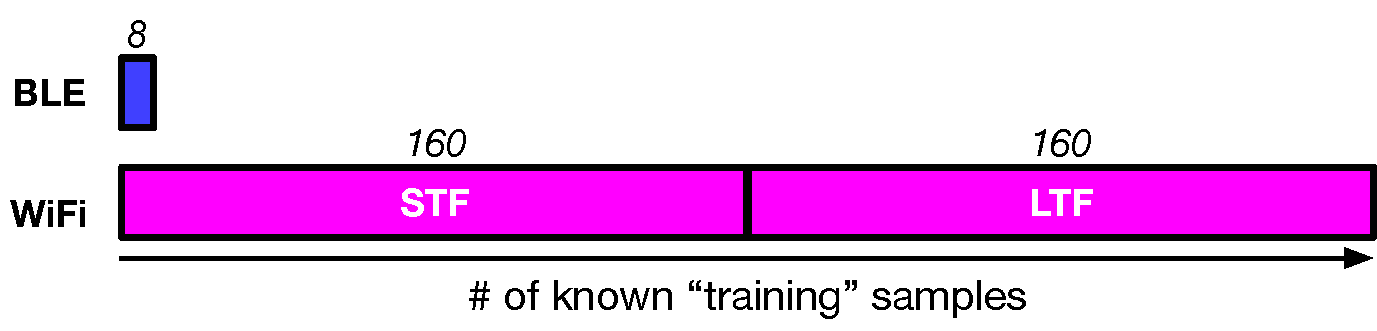
\includegraphics[width=\linewidth]{bletracking/plots/knownsamples}
    \caption{
      BLE packets have very few known samples for physical layer fingerprinting.
    \label{fig:2}
  }
\end{figure}

\vspace{0.5em} \noindent\textbf{Physical-layer fingerprinting:}
%
Physical layer fingerprinting is possible due to each radio having unique
hardware imperfections in its transmitter chain.
%
However, the design of BLE's physical layer is so simple that it is unlikely to
produce a unique physical-layer fingerprint. Also, even there were such a
fingerprint, it would be extremely difficult to extract that fingerprint from a
received BLE signal.
%
The reason is, BLE is an extremely low-energy protocol: BLE's physical-layer
signal is designed to require simple hardware to transmit and receive messages.
 
BLE signals are modulated basic Frequency Shift Keying (FSK) modulation. FSK
signals can be transmitted by a simple hardware phase-lock loop.
%
Such a simple transmitter will not have the complex hardware
impairments that have made it possible to fingerprint other mobile device protocols, namely WiFi~\cite{
vohuuusrp,
Brik_radiometric,
deviceID_kose}.
%
% Since these imperfections are
%caused by manufacturing variability, they can even produce a fingerprint for
%devices from the same make and model.
%
Additionally, BLE signals are so simple that they are difficult to recover a physical-layer fingerprint from.
%
%of a particular mobile
%device's radio is comparing known patterns in a signal received from that
%transmitter to the imperfect signal received from the transmitter.
%
Specifically, BLE transmissions do not require a significant number of known ``training''
samples for a receiver to use to correct for imperfections before decoding.
%  
These limitations make it difficult to apply existing physical-layer techniques~\cite{
vohuuusrp,
Brik_radiometric,
deviceID_kose,
Intrusion_hall,
suskitransient,
deeplearning_merchant,
lora_robyns,
gopalakrishnan2019robust}
to fingerprint BLE.
%
The problem is, these techniques have been developed for protocols, such as
WiFi, that require extremely accurate
corrections of impairments before they can be decoded.
%
%They require very accurate correction for imperfections in received signals
%before they can be successfully decoded.
%
Figure~\ref{fig:2} shows a comparison of the length of a typical
BLE beacon packet compared to a typical WiFi packet.
%
BLE packets only include 8 known symbols, whereas WiFi packets include 
a total of 320 known samples.

% Extra text {{{
\if 0
\paragraph{BLE Advertisement packets} BLE devices utilize advertisement packets
to indicate their presence to other devices in the vicinity. Advertisement
packets are short packets (at most 376 microseconds) which are frequently sent.
The packet length is shorter to save on energy and is typically 1/4 of the WiFi
packets. Advertisement packets include an 8-bit preamble, which is 10 $\times$
smaller compared to the WiFi preamble design. Furthermore, the packet consists
of a unique 48-bit identifier as advertising address (typically the hardware
MAC address of the radio), which is transmitted as part of the payload. Since
every packet contains the unique address, potential for tracking the device
became a concern. To alleviate this, Bluetooth SIG introduced address
randomization (as discussed in Section~\ref{sec:motivation}). Finally, the
complete advertising payload is appended with the CRC and is whitened or
scrambled. 

Hardware impairments in the transmitter chain which are caused by manufacturing
imperfections and tolerance, can make slight changes to the ideal signal that
should be sent by the device. Since these impairments are caused by
manufacturing imperfections, they are different even for the devices from the
same make and model. As a result, these hardware impairments can leave a unique
signature or fingerprint in the physical layer signal, that can be considered as
an identity for the device. Therefore, even though the MAC address changes
after a while, physical layer or radio frequency (RF) fingerprints remain the
same for a device which provides the attacker an opportunity to sniff the RF
fingerprints and identify the target at any time. Consequently, frequent
transmission of BLE packets can still cause a privacy threat even if MAC address
randomization is properly done. In this work, we aim to explore how practical
this attack could potentially be.
\fi
%}}}

\fi

%% Also that cellular skimmers are a thing http://newjersey.news12.com/story/38809657/consumer-alert-gas-station-gas-pump-credit-card-skimmers

% Also this is only going to get worse as the Bluetooth shimmer is now a thing https://www.sparkfun.com/sparkx/blog/2673

% "FICO, a credit scoring and analytics firm, noted that during the first half of 2017"

% https://www.muni.cz/en/research/publications/1073227
% https://www.muni.cz/en/research/publications/1362671
%
%European Financial Systems 2016, Proceedings of the 13th International Scientific Conference, year: 2016

%!TEX root = paper.tex
\section{Background}
\label{sec:background}

\begin{figure}
    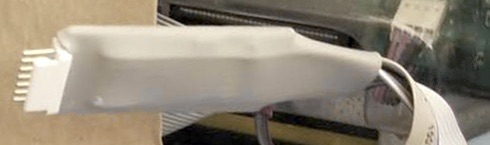
\includegraphics[width=0.95\linewidth]{skimmer/fig/wrapped-skimmer}
    \caption{An internal Bluetooth-based skimmer wrapped in grey tubing to blend in with the cabling inside the fuel pump. This skimmer
    was detected by \bluetana\ in Tempe, AZ.
%\noteby{NB}{Should we maybe put like a bigger picture with the entrails of the gas pump also visible?}}
}
\label{fig:wrapped-skimmer}
\end{figure}

\emph{Skimmers} are illicit devices that capture credit card magnetic stripe data when a card is used at a point-of-sale (PoS) terminal or automatic teller machine (ATM). External skimmers use a magnetic head concealed in a false
faceplate to read the magnetic stripe of a card as it is inserted into the real card reader. However, this paper is concerned
with a newer class of skimmers, called \emph{internal skimmers}, that are installed entirely inside a PoS
terminal or ATM, leaving no visual evidence of its presence~\cite{skimreaper2018}. Internal skimmers are attached inline to the cable that connects the
card reader to the main circuit board of the PoS terminal, tapping into the data and drawing power.
%
To make data collection easier, many internal skimmers include a Bluetooth-to-serial module that allows the
perpetrator to covertly collect the ``skimmed'' card data from a safe distance.
%
These skimmers are built using commodity hardware with a total unit cost of \$20 or less.

Fuel pumps
with a built-in PoS terminal have become a very popular target for such internal skimmers: they are unattended, easy
to access, and have poor physical security, which make it easy to install a skimmer without being noticed.
%
In a typical installation scenario, an attacker positions a van at a fuel station to block the station attendant's view of
the target pump (Excerpt in \ref{sec:appendix:cardsperskimmer}), opens the fuel pump using a common master key or crowbar, and clips a discreet gumstick-sized skimmer to the
ribbon cable between reader and main circuit board using a vampire clip (Figure~\ref{fig:wrapped-skimmer}). 
The entire process to install skimmer can
take less than 10 seconds~\cite{arizonareport}. The perpetrator can then return to the station with a 
smartphone, and without leaving their vehicle, connect to the skimmer using Bluetooth and download the card data.

\begin{figure}
    \centering
    \includegraphics[width=0.95\linewidth]{skimmer/fig/skimmer-example}
    \caption{Parts of a typical internal Bluetooth-based fuel pump skimmer. This skimmer
    was detected by \bluetana.}
    \label{fig:skimmer-example}
\end{figure}

\subsection{Internal Bluetooth Skimmers}
\label{sec:bkgd-skimhw}

The subject of our study are \emph{internal, Bluetooth-based skimmers} that are installed in fuel pump PoS
terminals. 
%
Figure~\ref{fig:skimmer-example} shows a typical Bluetooth skimmer, recovered from a fuel station in Southern California. This skimmer consists of a ``Teensy'' development board with an ARM Cortex-M4F
micro-controller and a Roving Networks \xspace{RN-42} Bluetooth-to-serial module. It also includes connectors 
for tapping into the wiring inside the pump (not shown). 

\paragraph{Connections} In the figure, the ribbon cable on the left intercepts or replaces the ribbon cable that connects the
magnetic stripe reader to the PoS terminal main board. The skimmer also uses this connection for power: the power and
ground pins of the Teensy (on far left of board, not visible in Figure~\ref{fig:skimmer-example}) are connected to
power and ground on the card reader cable. The ribbon cable on the right intercepts or replaces the ribbon cable from
the PoS keypad. This allows the perpetrator to capture additional card verification data, namely the debit card PIN
or credit card billing ZIP Code. Availability of a PIN code with a stolen debit card in particular, can increase its
value five-fold on the black market (Table \ref{tab:cardval}). However, not all skimmers capture keypad data.

Most gas station skimmers read the unencrypted data pulled from magnetic stripe readers.
%
Card issuers feel that removing sensitive data from the magnetic stripe on cards will help to solve
the problem~\cite{pcidss}.
%
Newer literature has demonstrated attacks on chip payment systems~\cite{bar2005known, bond2014chip}, and
law enforcement in Latin America have begun to find EMV skimmers that are Bluetooth enabled~\cite{krebshimmer,
customshimmer}.

\paragraph{Controller board} The skimmer pictured in Figure~\ref{fig:skimmer-example} used a Teensy micro-controller
development board equipped with a 120 MHz ARM Cortex-M4F micro-controller made by Freescale Semiconductor. By using a
development board, a skimmer requires only rudimentary electronic assembly: soldering wires to the development board.

However, skimmers have also been found using what appeared to be fully custom-designed boards. These are compact,
making them better for hiding in the dispenser. Examples of micro-controllers used in recovered skimmers include
Microchip PIC18F4550~\cite{sparkfunapp} and Atmel XMEGA128A4U~\cite{customshimmer}.

%\notefor{Nishant}{Please add additional examples of custom PCB skimmers from Web or skimmers we have seen ourselves; list \emph{exact} micro-controller and include a reference.}

%\noteby{NB}{Skimmers require minimal features on the micro-controller- low memory footprint[NB - Quote sparkfun website], two serial peripherals (to Bluetooth radio and mag reader), and a couple of GPIO/ADC(keypad) are all that are needed. In practice, skimmers recovered in the wild have been known to use various types of micro-controller boards.The first kind use readily available development boards, to enable fast prototyping. For example, the skimmer shown in figure uses a Teensy. In another kind of skimmers, criminals tend to simply re-purpose the micro-controller board on portable USB/Bluetooth mag readers, to use them as skimmers. The existing firmware can be used as is, but now to skim data. Finally, there are skimmers using custom boards based on a variety of micro-controllers (PIC18F, AtMega and others). While these boards take more effort to design and manufacture, the result is a compact skimmer which typically is hard to spot.}


\paragraph{Storage} The Teensy board also has a microSD card slot for additional data storage. Skimmers built on custom PCBs have also used flash and EEPROM ICs for storage. The storage capacities vary across designs, with examples using the PCT25VF032B (32-Mbit)~\cite{customshimmer} and M25P16VP (16-Mbit)~\cite{sparkfunapp}.

\paragraph{Bluetooth module} The skimmer shown in Figure~\ref{fig:skimmer-example} uses a Roving Networks RN-42 module, an inexpensive Bluetooth-to-serial module found in many skimmers. In Section~\ref{sec:bluetana:tool} we describe characteristics of popular Bluetooth-to-serial modules used in recovered skimmers for wireless data exfiltration. On the Bluetooth side, a Bluetooth-to-serial module provides a Serial Port Peripheral interface, which most operating systems recognize as a Bluetooth modem and instantiate a serial device for it. Operating systems will create a corresponding serial device, allowing user-space applications, namely a criminal's card dumping application, to communicate with the module. On the hardware side, a Bluetooth-to-serial module provides a TTL-level receive and transmit pin, allowing it to interface to any micro-controller UART. The module this allows even the simplest micro-controller to communicate via Bluetooth with a host device. The 2.4GHz Bluetooth antenna is included on the module's circuit board (exposed area to the left of the metal shield for the module shown in Figure~\ref{fig:skimmer-example}), so the antenna is also hidden.

Bluetooth-to-serial modules generally require no configuration, however, most
can be reconfigured using Hayes-style modem AT commands. In
Section~\ref{sec:bluetooth:skimmers} we describe the configuration capabilities
of popular modules. Notably, all of the Bluetooth-to-serial modules we found in
skimmers support changing the device MAC address, Bluetooth device name,
changing the pairing password, and the ability to become non-discoverable once
paired.

\subsection{Economics of Carding}
\label{sec:background:money}
Stealing and monetizing stolen credit and debit card data, called \emph{carding} by its practitioners, is a well-studied
form of financial fraud, however, reliable estimates of losses resulting from a single skimmer are difficult to find. To the criminal operating a skimmer, the expected revenue per skimmer breaks down as:
%
\[W = \textrm{(card value)}
\times \textrm{(cards per day)}
\times \textrm{(days deployed)}.\]
%\[W = \underbrace{\textrm{(card value)}}_{P}
%\times \underbrace{\textrm{(cards per day)}}_{Q}
%\times \underbrace{\textrm{(days deployed)}}_{D}.\]

Of these, we found published estimates for only the first two quantities, and very little about skimmer lifetimes. Here, we summarize the available data with the goal of estimating the losses incurred by a single skimmer.

\paragraph{Card value} To monetize stolen credit card data, skimmer installers have two options: sell the data on the black market, or cash out the cards on themselves. Based on our survey of sites selling stolen card data, black market prices for stolen cards fall in the \$10--220 range, depending on whether the card is a debit or credit card, and whether it comes with a PIN (for debit) or billing ZIP code (for credit). Table~\ref{tab:cardval} provides a summary of these prices with references. 

\begin{table}
\begin{tabular}{l@{\quad}lrl}
    \toprule
    \multicolumn{2}{l}{\colname{Scheme}} & \colname{Value} & \colname{Reference} \\
    \midrule
    \multicolumn{2}{l}{\textbf{Black market price}} \\
    & Debit, no PIN & \$20--30 & \cite{meccadumps,sellcvv,dumpsto, dumpsPrtShip} \\
    & Debit with PIN & \$110--220 & \cite{legitshop, sellcvv, dumpsPrtShip} \\
    & Credit, no ZIP & \$10--25 & \cite{meccadumps,sellcvv,dumpsto, dumpsPrtShip} \\
    & Credit with ZIP & \$25--60 & \cite{meccadumps,sellcvv,dumpsto, dumpsPrtShip} \\
    \multicolumn{2}{l}{\textbf{Cash-out value}} \\
    & Credit or Debit (standard) & \$400--800 & \cite{makingFirstMoney, cardingNewbieGuide, howToSucceedInStore, viceInterviewWithCarder} \\
    & Credit (premium) & \$1,000 & \cite{cardingNewbieGuide, santandWithdraw, honeyMoneyTut}\\
   \multicolumn{2}{l}{\textbf{Bank and merchant loss}} \\
%   & DOJ & \$902 & \cite{harrell2017} \\
%   & Arizona W\&M & \$1,003 & \cite{arizonareport} \\
    & Credit & \$1,003 & \cite{arizonareport} \\
%   & ATM Skimming & \$650 & \cite{ATMIA} \\
    & Debit & \$650 & \cite{ATMIA} \\
    \multicolumn{2}{l}{\textbf{Consumer liability}} \\
    & Debit (> 60 days) & unlimited & 15~USC~1693g \\ % \cite[\S1693g]{15uscode} \\
    & Debit (< 60 days) & max \$500 & 15~USC~1693g \\ % \cite[\S1693g]{15uscode} \\
    & Debit (< 2 days) & max \$50 & 15~USC~1693g \\ % \cite[\S1693g]{15uscode} \\
    & Credit & max \$50 & 15~USC~1643 \\ % \cite[\S1643]{15uscode} \\
     \multicolumn{2}{l}{\textbf{Prosecuted loss}} \\
%   & USSC & \$500 & \cite{ussc-guidelines} \\
    & Credit or debit & \$500 & \cite{ussc-guidelines} \\
     \multicolumn{2}{l}{\textbf{Court documents}} \\
     & Credit & \$362--400 & \cite{hristov,cristea,alisuretove,mekhakian} \\
     & Debit & \$665--1132 & \cite{estrada,aqel} \\

    \bottomrule
\end{tabular}

\caption{Value of stolen credit and debit cards.}
\label{tab:cardval}
\end{table}

Criminals can also cash out the cards themselves. Debit cards with a PIN are often cashed out by withdrawing money from an ATM, while credit cards are often cashed out by purchasing high-value merchandise (e.g. iPhones) and re-selling them. Reported cash-out values for debit and credit cards range between \$400 and \$1,000, depending on credit limit associated with the card.
%
We also conducted a survey of cash-out values reported in court documents involving skimmers.\footnote{We surveyed only documents available without fee from Court Listener.} Several cases reported specific cash-out values, rather than ranges. The debit card cash-out values were \$1132~\cite{hristov}, \$444~\cite{cristea} \$665~\cite{alisuretove}, \$1354~\cite{mekhakian}. The credit card cash-out values were \$362~\cite{aqel} and \$400~\cite{estrada}.

Losses due to credit and debit card fraud are borne largely by banks and merchants. This is likely because consumer liability for fraud in the U.S. is limited to \$50 for credit cards, and \$50 or more for debit cards (depending on how quickly the consumer reports the fraud).  Industry estimates for losses per-card incurred by banks are \$650 for debit cards and, \$1,003 for credit cards~\cite{arizonareport,ATMIA}. The U.S. Sentencing Commission estimates per-card losses at \$500 or more.

\paragraph{Cards per day} The number of cards a skimmer captures each day
depends on the number of transactions at that pump, which will vary by station.
Rippleshot, a payment fraud prevention service, states: ``a single compromised
pump can capture data from roughly 30--100 cards per day''~\cite{rippleshot}.
The lower end Rippleshot's estimate agrees with the estimate of 20--50 cards
per day we received from U.S. law enforcement agents. In addition, we found two
court documents that report criminals captured 25~\cite{estrada} and
30~\cite{alisuretove} cards per day.
%
We also studied 10 skimmers recovered from the field, which we were told were used and wiped daily. We found an average of 20 cards per skimmer, divided
evenly between debit and credit cards.\footnote{These skimmers were provided to
us because they were removed by the station owner, rather than LE, making them
unsuitable for use as evidence.}

\paragraph{Days deployed}  Internal skimmers are not limited by battery life
and can remain in operational indefinitely, because they draw power from the
PoS circuitry, Skimmer lifetime, then, is limited only by how long they can
remain undetected. Unfortunately, there is little reliable data on this. Our
only direct experience is our discovery of a pair of skimmers that remained
undetected for six months (Section~\ref{sec:blu:identify}). However, LE
informed us that criminals may leave skimmers in gas pumps after only a few days of retrieving 
card data and moving on to another location. Given the very limited data available on
skimmer lifetimes, we instead consider skimmer value \emph{per day of
operation}.

\paragraph{Cashout success rate}

Our analysis of court documents revealed that criminals are often unsuccessful
when trying to cashout a skimmed card. This may be due to a variety of reasons,
such as the following: incorrectly reading card data, hitting daily withdrawal
limits, and activating fraud alerts. Several cases mentioned that criminals
were not successful in cashing all skimmed cards. One case mentions a specific
cashout success rate of 47\%~\cite{mekhakian}.%, and the other was 50\%~\cite{rodriguez}.

\paragraph{Total skimmer value}

Finally, we estimate the range of per-day revenue from a skimmer based on the
prior figures. Our low end estimate is \$4,253 (25 cards per day, cashout of
\$362 per card, and 47\% cashout success rate), and our high end estimate is
\$63,638 (100 cards per day per day, \$1,354 cashout per card, and cashout success rate of
47\%).

\begin{comment}
Taking 30 cards per day, the lowest value in the Rippleshot range and near the middle of the estimate from law enforcement, and \$500 per card, the figure estimated by law enforcement officers and consistent with other estimates of cash-out value, places the value of each skimmer to the criminal at \textbf{\$15,000 per day}.

We compare this with a separate estimate obtained from information in court documents. Knowing that there is an equal distribution of credit and debit cards per skimmers, the average cashout value is at \$615 per card. With an average of 27 skimmer per card per day, and a lower bound success rate of 47.1\% in cashing out, the value of skimmer per day to the criminal stands at \$7820 per day.
\end{comment}

\begin{table}
\centering
\small
% Converted to vertical format by Aaron to manage space
\if 0
\begin{tabular}{lrrrrrrrrr}
\toprule
& \multicolumn{1}{c}{SD}
& \multicolumn{4}{c}{Arizona}
& \multicolumn{4}{c}{Florida}
\\
\cmidrule(lr){2-2}
\cmidrule(lr){3-6}
\cmidrule(lr){7-10}
%
\colname{Parameter}
& \colname{FY18}
& \colname{2016} & \colname{2017} & \colname{2018} & \colname{All}
& \colname{2016} & \colname{2017} & \colname{2018} & \colname{All}
\\
\midrule
Recovered skimmers
& \sdfyXVIIIskimmers
& \azXVIskimmers & \azXVIIskimmers & \azXVIIIskimmers & \azALLskimmers
& \flXVIskimmers & \flXVIIskimmers & \flXVIIIskimmers & \flALLskimmers
\\
Skimmed stations
& \sdfyXVIIIsksta
& \azXVIsksta & \azXVIIsksta & \azXVIIIsksta & \azALLsksta
& \flXVIsksta & \flXVIIsksta & \flXVIIIsksta & \flALLsksta
\\
Skimmers per incident
& \sdfyXVIIIskperinc
& \azXVIskperinc & \azXVIIskperinc & \azXVIIIskperinc & \azALLskperinc
& \flXVIskperinc & \flXVIIskperinc & \flXVIIIskperinc & \flALLskperinc
\\
Skimmers per million
& \sdfyXVIIIskpercap
& \azXVIskpercap & \azXVIIskpercap & \azXVIIIskpercap & \azALLskpercap
& \flXVIskpercap & \flXVIIskpercap & \flXVIIIskpercap & \flALLskpercap
\\
\bottomrule
\end{tabular}
\fi

\begin{tabular}{lcccc}
  \toprule
	\multicolumn{1}{p{1.5cm}}{\colname{Location \& Year}}          &
	\multicolumn{1}{p{2.0cm}}{\centering \colname{Recovered skimmers}}     & 
	\multicolumn{1}{p{1.5cm}}{\centering \colname{Skimmed stations}}       & 
	\multicolumn{1}{p{1.6cm}}{\centering \colname{Skimmers / \newline station}}     &
	\multicolumn{1}{p{1.8cm}}{\centering \colname{Skimmers / \newline $10^6$ people}}   \\
	\midrule
	\multicolumn{4}{l}{\textbf{San Diego}} & \\
	\hspace{0.4cm}FY 2018 & \sdfyXVIIIskimmers & \sdfyXVIIIsksta & \sdfyXVIIIskperinc & \sdfyXVIIIskpercap \\

  \multicolumn{4}{l}{\textbf{Arizona}} \\
	\hspace{0.4cm}2016 & \azXVIskimmers & \azXVIsksta & \azXVIskperinc & \azXVIskpercap \\
	\hspace{0.4cm}2017 & \azXVIIskimmers & \azXVIIsksta & \azXVIIskperinc & \azXVIIskpercap \\
	\hspace{0.4cm}2018 & \azXVIIIskimmers & \azXVIIIsksta & \azXVIIIskperinc & \azXVIIIskpercap \\
	\hspace{0.4cm}\textit{All}  & \azALLskimmers & \azALLsksta & \azALLskperinc & \azALLskpercap \\

  \multicolumn{4}{l}{\textbf{Florida}} \\
  \hspace{0.4cm}2016 & \flXVIskimmers & \flXVIsksta & \flXVIskperinc & \flXVIskpercap \\
	\hspace{0.4cm}2017 & \flXVIIskimmers & \flXVIIsksta & \flXVIIskperinc & \flXVIIskpercap \\
	\hspace{0.4cm}2018 & \flXVIIIskimmers & \flXVIIIsksta & \flXVIIIskperinc & \flXVIIIskpercap \\
	\hspace{0.4cm}\textit{All}  & \flALLskimmers & \flALLsksta & \flALLskperinc & \flALLskpercap \\

  \bottomrule
\end{tabular}

\caption{Prevalence of skimming in three regions of the U.S.}
\label{tab:wildskims}
\end{table}

\subsection{Skimmers Recovered in the Wild}
\label{sec:skimmersinwild}
To understand the prevalence of skimmers in the wild, we obtained data on recovered skimmers from three regions in the United States: San Diego and Imperial counties of California, with a combined population of 3.5 million; the state of Arizona, with a population of 7 million inhabitants; and the state of Florida, with a population of 21 million inhabitants. Table~\ref{tab:wildskims} summarizes the statistics. We note that these numbers do not represent \emph{all} recovered skimmers. For San Diego and Imperial counties, our statistics represent the number of skimmers found by or reported to a U.S. federal law enforcement agency. For Arizona and Florida, our statistics represent skimmers found by or reported to the AZWMSD and the Florida Department of Agriculture and Consumer Services.

The number of recovered skimmers has increased from 2016 to 2018 in both Florida and Arizona. The total number of skimmers recovered in 2018 across the three geographic regions is significant: if each skimmer operated for just one day, we estimate their total monetary impact would be ~\skimmerfraudXVIIIUSA. Yet, as the skimmers-per-million people number shows, the possibility of an average consumer encountering a skimmer at a gas station is quite small.

%!TEX root = paper_main.tex

\section{BLE Tracking Toolkit}
\label{sec:methodology}

In this section I present a high-level overview of the algorithm we use in this work to estimate the physical-layer properties of the BLE transmitters.
%
The mathematical details of the algorithm are beyond the scope of this dissertation, and therefore I only present the high level intuition to obtaining high-precision fingerprints from BLE beacons.

The hardware imperfections that lead to the fingerprint arise from the underlying manufacturing variations in BLE transmitter hardware.
%
These manufacturing variations lead to non-idealities in the received BLE beacon signals, which we can measure to derive the fingerprint.
%
In particular, most mobile devices feature an integrated single-chip WiFi+ BLE transmitter, which has a shared \iq frontend.
%
Therefore, the BLE transmissions are impacted by the same hardware imperfections as the WiFi transmitter.
%
For our work, we explore the following specific hardware imperfections:
\begin{enumerate}
    \item \textbf{CFO: } The Carrier Frequency Offset (CFO) is a shift in the carrier frequency from the ideal channel value. This arises due to the frequency error of the crystal oscillator that is used to generate the carrier signal that feeds into the mixer in the RF frontend.
    \item \textbf{\iq imperfections :} \iq Offset happens due either the leakage of the carrier signal onto the transmitter output due to non-idealities of the mixer hardware, or due to an DC offset on the baseband signals. \iq Imbalance is a deviation in amplitude and phase of transmitted signal, due to the mismatch between similar analog components on the in-phase and quadrature-phase paths.
    
\end{enumerate}
\begin{figure}
    \centering
    \captionsetup{justification=centering}
    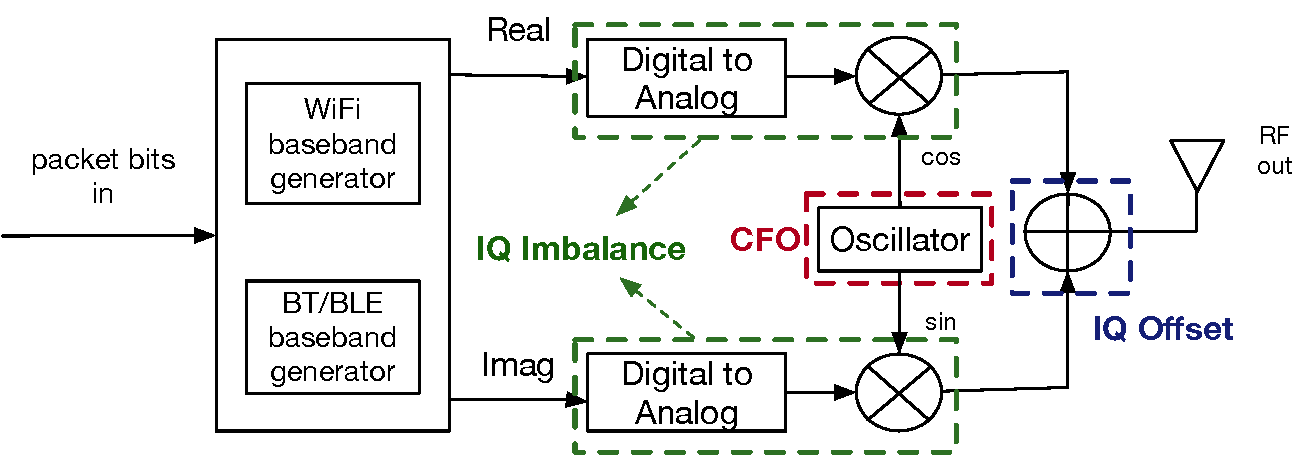
\includegraphics[width = 0.8\linewidth]{bletracking/plots/IQchain.pdf} 
    \caption{Architecture of WiFi/BLE combo chipsets}
    \label{fig:iq_arch}
\end{figure}
Figure~\ref{fig:iq_arch} shows the architecture of a typical BLE transmitter, and the sources of the imperfections described above.

Unfortunately, we can't reuse techniques from prior work on WiFi physical-layer fingerprinting to measure these properties precisely for Bluetooth LE. 
%
Prior techniques rely on the presence of a long known sequence or preamble as a reference to measure the signal distortions due to CFO and \iq imperfections accurately
%
BLE has a very short preamble and that leads to extremely inaccurate estimates of CFO and \iq from prior techniques.
%

However, a key insight about BLE decoding helps us.
%
Unlike WiFi, BLE uses simpler GFSK modulation and does not require us to compensate CFO and \iq imperfections before decoding.
%
Consequently, we can decode the entire BLE beacon packet and obtain the full bit sequence correctly.
%
This bit sequence can be used to create a reference signal which is much longer (packet length), and that can provide us improved estimates for our fingerprint.

With a longer reference signal available as a starting point, the fingerprint estimation algorithm estimates the hardware imperfections. 
%
Starting with the initial pure signal, the algorithm iteratively adds CFO and \iq imperfections until our pure starting signal looks similar to the received signal.
%
To do so it models the imperfection estimation as an optimization problem, with the BLE signal modelled under impact of the imperfections.
%
Using this approach, we were able to achieve high precision estimates as compared to using just 8 bits of preamble.
%
Furthermore, the estimates over a packet are obtained as an average across all the raw samples in the packet, which minimizes impact of SNR changes, resulting in robust estimates of CFO and \iq imperfections.

Finally, for the actual tracking attack the attacker estimates CFO and \iq from multiple beacon packets from the same device.
%
The actual fingerprint is represented as a distribution of CFO and \iq across multiple packets.
%
When actually tracking the target at the destination, the statistical distance of the distributions of a newly observed device and target are compared against a threshold.
\section{Real-world challenges to physical-layer identification}
\label{sec:results2}
Using our high-precision fingerprint technqiue, we perform an empirical analysis in lab conditions to understand the limitations of this physical layer identification.
%
There are five primary challenges that limit the effectiveness of tracking
BLE devices based on their physical-layer fingerprint. 
%
For each challenge, we
perform controlled experiments or theoretical analysis to investigate how significantly they affect
fingerprinting accuracy in practice, and in turn the ability of an attacker to uniqely identify their target. 
%
We found that BLE tracking attacks are
likely to be feasible in practice. 
%
However, the attacker's ability to identify a
specific device reliably will vary depending on several factors that are out of
their control.

\subsection{Uniqueness of BLE fingerprints} %{{{
\label{sec:similarity}

\begin{figure}
    \centering
    \captionsetup{justification=centering}
    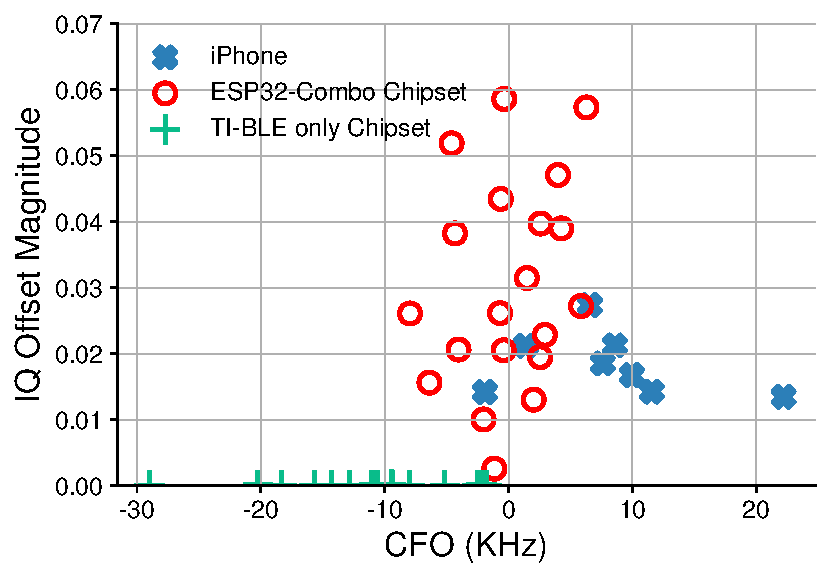
\includegraphics[width = 0.6\linewidth]{bletracking/plots/cfoiq_iphone_esp_ti2.pdf} 
    \caption{Comparing the fingerprints of 48 BLE chipsets}
\label{fig:cfoiq}
\end{figure}

BLE transmitters must have unique imperfections if an attacker wants to
differentiate their target from other nearby devices.  To evaluate how
similar BLE fingerprints are in practice, we compare the fingerprint of  many
devices across three different popular BLE chipsets. Specifically, we
captured the fingerprint of eight recent iPhones with WiFi+BLE combo
chipsets, 20 ESP32 WiFi+BLE microcontroller chipsets, and 20 TI CC2640
BLE-only chipsets used in low-power devices (e.g., fitness trackers).  We
captured 100 packets using a high-quality SDR (USRP N210) from each of these
devices in a controlled environment (i.e., an RF isolation chamber). We
computed the fingerprint of each device across all 100 packets using the methodology described in
the previous section.

Figure~\ref{fig:cfoiq} shows the mean of the fingerprint metrics for each of
the 48 devices. We plot only the CFO and \iq offset metrics to simplify the
visualization, adding \iq imbalance does not change the conclusions of the
experiment. Overall, most of the 48 devices have unique fingerprints. However, there
are a few devices that have similar fingerprints, making them more difficult to uniquely identify. The distribution of
device fingerprints also appears to be dependent on the chipset.
%All devices appear to have
Namely, there are striking differences in how the \iq offset metric is
distributed between different chipsets.
For instance, the ESP32 devices have a much
larger range of \iq offsets than the iPhones, which may be
because ESP32s are low-end chipsets compared to the
high-performance WiFi+BLE combo chipsets used in iPhones.

\begin{figure}
    \centering
    \captionsetup{justification=centering}
    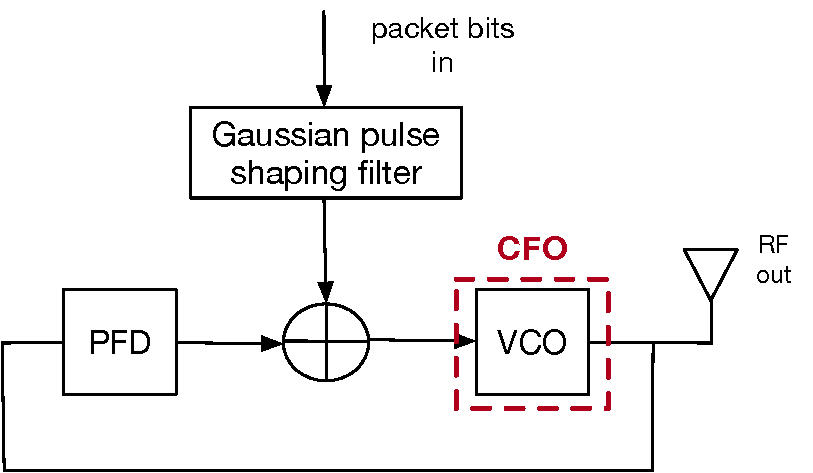
\includegraphics[width = 0.6\linewidth]{bletracking/plots/dpll.pdf} 
    \caption{TI's BLE-only transmitter. This is not an \iq modulator.}
    \label{fig:dpll}
\end{figure}

Surprisingly, the TI BLE-only chipsets all have negligible \iq offset.
Recall in Section~\ref{sec:methodology}, we described how unlike WiFi, BLE is
not an inherently \iq modulated protocol; therefore, the TI's BLE-only
chipset may have \iq offset because it may not use an \iq modulator.  We
confirmed this suspicion by finding a technical report that describes the
TI BLE chipset radio architecture: it uses a PLL-based 
(non-\iq) modulator~\cite{pllarchBLE}.

\subsubsection*{Summary} An attacker's ability to uniquely identify a target device's 
fingerprint depends on the BLE chipset it is using, as well as the
chipsets of the other devices nearby. Distinguishing devices
with the same chipset is likely more difficult than distinguishing 
devices with different chipsets. This may make tracking 
attacks difficult in practice because targets are likely to use the same popular devices (e.g.,
iPhone). %Although, if the target happens to be a device that is not common in that
%environment, they are likely to have a much more unique fingerprint.

%ability to identify a device totally depends on its inherent RF fingerprints.
%There are regions that include many devices with common fingerprints while some
%devices have a very unique and distinguishable fingerprints. Second, although
%most devices seem separable, the fingerprints of some of them are not that far
%from each other. Consequently, a coarse grained imperfection estimation
%algorithm may result in poor accuracy, which emphasizes employing a
%fine-grained imperfection estimation algorithm similar to the one introduced in
%this paper. Also any environmental effect such as noise which increases the
%imperfection estimation error or temperature variations which changes the
%fingerprints, can cause confusion in distinguishing the devices with close
%signatures.

%enough fingerprints to distinguish them. Also, these distributions of
%imperfections may be chipset model specific, some may be easier to distinguish
%than others.
%}}}

\subsection{Temperature stability of BLE fingerprints} %{{{
\label{sec:challenges:temperature} A device's BLE fingerprint must be stable
to track over time across multiple locations.  However, a device's CFO
may drift when the temperature of the device changes.  CFO is a
product of imperfections in the crystal oscillator used to generate the
transmitter's center frequency (e.g., 2.480~GHz), and the frequency error of
a crystal oscillator has a well-defined relationship with its temperature
called the ``Bechmann curve''. The relationship between temperature changes
and \iq imperfections is not as well understood as with CFO.

Smartphones are particularly exposed to temperature variations. Their
internal temperature can significantly change due to internal components heating up (and cooling down) when activity changes, and
they also experience a variety of ambient temperatures~\cite{fireinyourhands}.
However, it is possible that smartphones 
do not have instability in their BLE transmissions. The impact of temperature
on CFO is dependent on the cut angle and face of the crystal~\cite{temp_cfo1},
and smartphones may use high-quality crystals that have less frequency drift due to temperature changes.
Also, smartphones may use temperature compensated
crystals as they may be required for high-data rate cellular communication chipsets.
 

%We expect the impact
%of these temperature differences to affect CFO much more than they affect I/Q modulation imperfections is likely to
%be less significant than they are on CFO.

\begin{comment} On the other hand, IQ offset due to carrier leakage is
  frequency independent, and shouldn't be impacted.  It is well known that CFO
  impairment varies with the temperature. A natural question is how robust is
  the attack with temperature. In this section, we specifically consider
  variation in the fingerprint due to temperature and evaluate in detail, if
  during normal operation does the temperature change significantly. An
  interesting observation in most typical operating conditions our attack would
still work.
\end{comment}

We performed controlled experiments to observe how temperature affects CFO and \iq offset of a typical smartphone. We tested the effects of internal components changing temperature by playing a
graphics-heavy game (Asphalt 9), and the effects of ambient temperature by putting an idle phone into a user's pants
pocket.
%
Our test device was a common smartphone, a Moto G6, and it was running a COVID--19 contact tracing app to generate BLE transmissions.
%During the test, the 
%the phone was in a normal operation state (WiFi, LTE, Bluetooth all on). 
%
Each test ran for 15 minutes. During the tests we captured the fingerprint metrics from each BLE packet with a USRP N210.
%
Simultaneously, we also captured readings from all the internal temperature sensors of the device.
We only present the temperature sensor data that most closely correlated with the changes in
CFO, which was the Power Management Integrated Circuit's temperature sensor.

\begin{figure}
\begin{subfigure}{0.48\textwidth}
    %\centering
    %\captionsetup{justification=centering}
    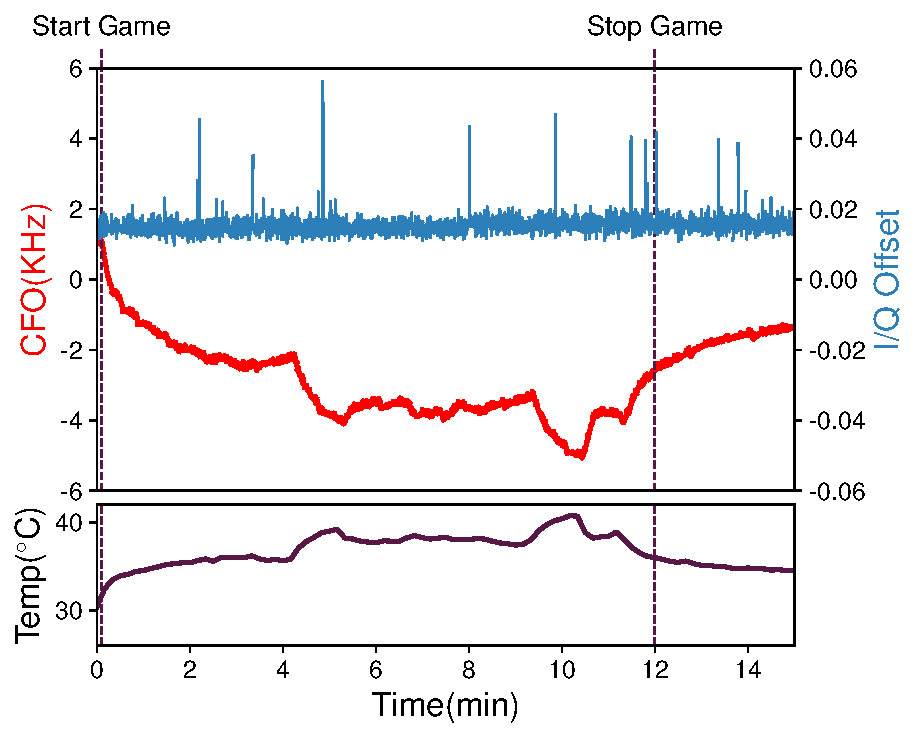
\includegraphics[width = \textwidth]{bletracking/plots/gameplay_temp_cfoiq.pdf} 
    \caption{}
    %\caption{Metric stability while playing a GPU-intensive game}
    %\label{fig:exert_cfo}
\end{subfigure}
\hfill
\begin{subfigure}{0.48\textwidth}
    %\centering
    %\captionsetup{justification=centering}
    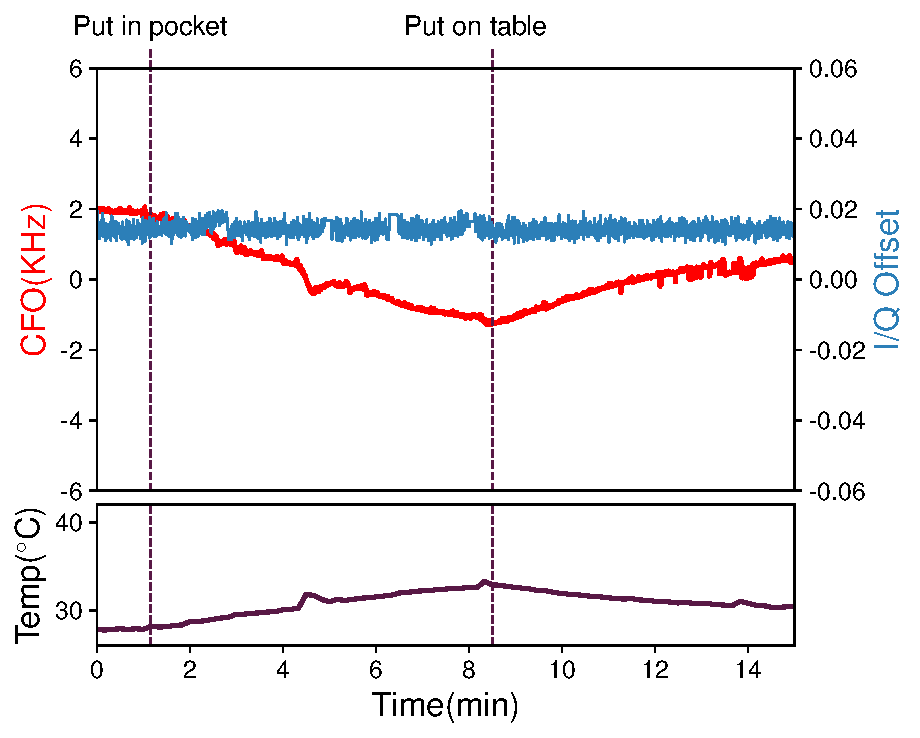
\includegraphics[width = \textwidth]{bletracking/plots/idle_temp_cfoiq.pdf} 
    \caption{}
    %\caption{Metric stability while putting the phone in a pocket}
    %\label{fig:idle_cfo}
\end{subfigure}
\captionsetup{justification=centering}
\caption{Stability of CFO and \iq offset when (a) playing a GPU-intensive game and (b) putting the phone in a pocket}
\label{fig:stability_cfo_temp}
\end{figure}

Figure~\ref{fig:stability_cfo_temp} shows the per-packet
variation in CFO and IQ offset during the 15-minute tests. We do not show the
variation in I/Q imbalance as it as we found it has a similar relationship to
temperature as I/Q offset. 
%
For the game experiment, we observe that the CFO
has a linear relationship to the changes in
temperature. When the game begins, the CFO increases, and when the game ends, it decreases.
At the peak internal temperature (+10\textdegree C above baseline),
we observe a significant CFO deviation (7~kHz).
%
%Finally, when the user stops playing the game, the temperature as well as CFO
%slowly taper off towards their initial values.
%
For the in-pocket experiment, the peak change in CFO is much
less than the game experiment (2~kHz). However, it is
still significant enough to introduce confusion with other devices that have
similar I/Q metrics (Figure~\ref{fig:cfoiq}).
Finally, figure~\ref{fig:stability_cfo_temp} show that I/Q offset
(and I/Q imbalance which is not shown) does not correlate with
temperature in both the cases.

\subsubsection*{Summary} 
Device temperature changes significantly change the CFO
a smartphone, but not the \iq imperfections. If an attacker tries to track a device when it is under
heavy use, it will need to allow for significant differences in CFO from the
initial fingerprint, which may result in increased confusion with other nearby
devices. Also, putting an idle device in a user's pocket changes the CFO
significantly enough to cause confusion as well.  Ideally, an attacker would
both get an initial fingerprint, and try to identify the device, in the of the most common use case for the device: idle in
the user's pocket. 
%If a device experiences a significant change in ambient temperature, the
%attacker would have to acquire a new fingerprint, and if the device is active, when its identified.

%}}}

\subsection{Differences in BLE transmitter power} %{{{

BLE transmit power affects how far away an attacker can track a target.  If
some devices have lower transmit power, it is more difficult for an
attacker to capture their beacons.  One may assume that all similar devices
(e.g., smartphones) would use similar transmit power---especially when they are running the same popular
app. In particular, we would expect similar transmit power for
the same contact tracing apps, where transmit power correlates with distance where the
contact occurred.  However, transmit power is configurable: BLE
APIs on mobile devices allow applications to set their beacon transmit power
to match the needs of the application.

We measured the received SNR of BLE beacons from several popular smartphones while they were
running the Apple/Google COVID--19 contact tracing app.  The measurement was
performed with a USRP N210, and all the phones were placed at the same distance (15 feet) from the
USRP. We performed this measurement on five different phones, running latest
version of iOS and different versions of Android. We installed the same
official California COVID--19 contact tracing app on all the devices. Then,
we averaged the SNR over 100 received packets
from each of the devices.

Figure~\ref{fig:txpwr} shows that the iPhone~8 has an SNR 10~dB higher
than all other Android phones we tested. Therefore, the iPhone's BLE beacons
are likely to be received considerably farther away than the other devices.
Anecdotally, we observed that an iPhone's COVID--19 contact tracing beacons
7~meters farther than any of the Android devices we tested\footnote{Including other versions of the iPhone available at the time (e.g., Xr).}.

\subsubsection*{Summary} There can be significant differences in BLE transmit power
across devices, and even across apps running on devices. We observed
that iPhones transmit COVID--19 contact tracing beacons with significantly higher
power than Android devices.  Consequently, attackers may be able to track
iPhones from a farther distance than Android devices.
%}}}

\subsection{Quality of an attacker's sniffer radio} %{{{
    \label{sec:hadi:sdr}

\begin{figure}
    \centering
    \captionsetup{justification=centering}
    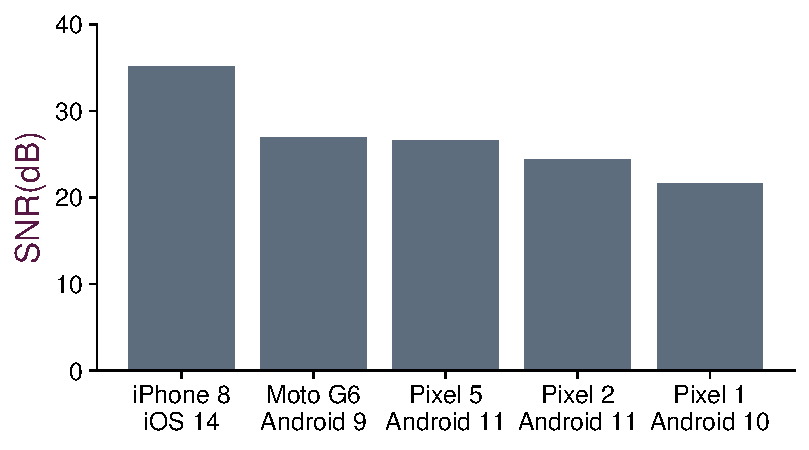
\includegraphics[width=0.6\textwidth]{bletracking/plots/phone_power_barplot}
    \caption{SNR of COVID contact tracing beacons across devices}
    \label{fig:txpwr}
    \end{figure}
    
\begin{comment}
Physical-layer fingerprinting attacks can require an expensive high-quality Software-Defined Radio (SDR) to execute.
%
The more expensive the required SDR is, the fewer locations an attacker can deploy them to track their target.
%
On the other hand, the problem is that an SDR's receiver
chain adds signal imperfections to the received signals.


Recently, several low-cost SDRs have
become popular among hobbyists.
%
However, the stability of their receivers'
imperfections are unknown. We evaluate if one of the least expensive SDRs has
sufficient imperfection stability for BLE device tracking.
\end{comment}

Physical-layer fingerprinting attacks can require an expensive high-quality
Software-Defined Radio (SDR) to execute. The problem is, an SDR's receiver
chain adds signal imperfections to the transmitted signals. If the SDR's
imperfections are unstable, they can make it difficult to identify a device
based on its previously captured fingerprint. On the other hand, the more expensive the required SDR is, the fewer locations an attacker can
deploy them to track their target. 

Recently, several low-cost SDRs have
become popular among hobbyists. However, the stability of their receivers'
imperfections are unknown. We evaluate if one of the least expensive SDRs has
sufficient imperfection stability for BLE device tracking.

We compared the fingerprinting metrics captured by a high-end SDR, USRP N210 (\$3,400), and a low-end SDR, LimeSDR-Mini (\$179).
To make the comparison fair, we sent BLE packets from a single iPhone device to both SDRs simultaneously.
We computed the average and standard deviation of
our metrics to evaluate if the two devices observe the same absolute imperfections, and if they have similar metric stability.
Similar to prior experiments, we captured 100 beacons to compute these
distributions.

\subsubsection*{CFO} The USRP observed a mean of -4.78~kHz and a standard
deviation of 102~Hz, while the Lime-SDR observed a lower mean of -8.07~kHz
but with a similar standard deviation of 114 Hz. The difference is in the mean CFO is likely due
to manufacturing variations in the SDR's crystal oscillators. Both radios
however use a TCXO-based oscillator, therefore their CFO measurements will be stable even if the SDR's temperature changes.

\subsubsection*{\iq metrics} A similar conclusion can be drawn about the
differences between the observed I/Q metrics. The USRP observed an average I/Q
offset magnitude of 0.0145 and standard deviation of 0.0017. While the Lime-SDR
observed an average of 0.0203 but with a similar standard deviation 0.0030. 
The \iq imbalance was surprisingly similar across both devices, with a mean
amplitude of 0.991 for the USRP and 0.987 for the Lime-SDR, the corresponding standard deviations
were similar too (0.0016 and 0.0021).

\subsubsection*{Summary} Attackers can use lower-cost (\$179) hobbyist-grade
SDRs to do physical-layer attacks, but they will likely have to calibrate the
differences between their SDRs before they deploy them.
%}}}

\subsection{Mobility of target device} %{{{
\label{sec:hadi:mobility}

Physical-layer tracking would be impossible if the BLE fingerprint of BLE device
changes as it moves from one physical location to another.  Specifically,
fingerprints may change due to differences in the target's physical environment
(e.g., multipath in one room vs. another), and differences in
motion of the target (e.g., walking vs. driving).
    
\subsubsection*{Physical environment} A change in the physical location of the
target can alter the received signal's SNR due to changes
multipath conditions. However, we observed that this appears to have 
an insignificant impact on BLE fingerprinting metrics. 
%
We have observed through experiments that above a
certain minimum SNR ($\sim$10 dB), changes in SNR do not impact
identification accuracy.

\subsubsection*{Speed of Motion} A moving BLE device may experience a
velocity-dependent frequency offset due to the Doppler
effect~\cite{nasadoppler}. While this may cause a slight drift in the CFO of
the BLE target device, the impact is not significant for the frequencies that
BLE operates at. 

For example, if a BLE device is moving at a velocity of 80
kilometers per hour,  and the receiver is stationary, the Doppler frequency
offset at 2.4~GHz is about 180 Hz. This is only \~50\% of the median of standard
deviation of CFO for BLE devices we observed in the field
(Figure~\ref{fig:cfo_comp}). Therefore, even at
relatively high speed motion, the Doppler shift doesn't impact an attacker's
ability to track devices.
    
\subsubsection*{Summary} 
Changing location, or speed, of BLE device has an insignificant impact on the
attacker's ability to accurately fingerprint and identify a target device.
    
    %\begin{figure}[t!]
        %\centering
        %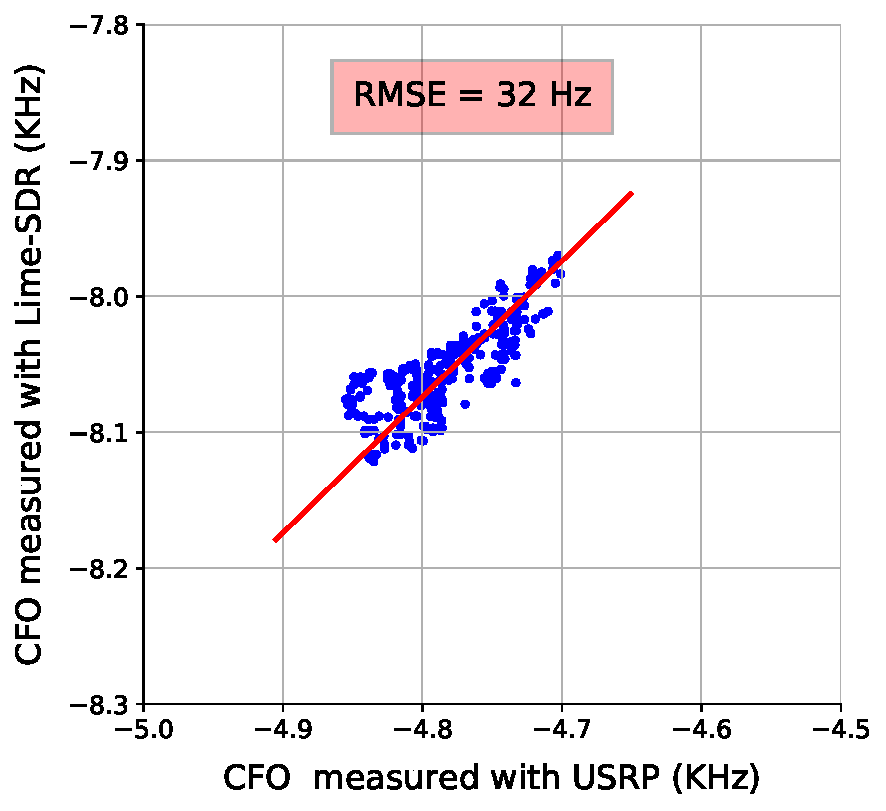
\includegraphics[width = \linewidth]{plots/cfo_scatter_sdr.pdf}
        %\caption{CFO Comparison of two SDR receivers. CFO values of 1000 packets from a device were measured with a Lime-SDR and an USRP. The RMSE is 32 Hz which indicates it is possible to use a different receiver as long as the CFO between receivers is calibrated compensated.}
        %\label{fig:cfo_scatter_sdr}
    %\end{figure}
%}}}
    

%!TEX root = paper_main.tex
\section{Field Evaluation}
\label{sec:results}

% LIMITATION: WE HAD TO DO IT OVER 15minutes or we don't know who is the same device
% Threshold setting: The distance between your device and the device you are looking at
% Q1 - C1: \textit{what is the chance that we confuse a device that is not our target with a device that we are looking for?}
%  - Have a target and chose any single of the 160 and see if that's your target, check if it's not happening for each device.
%  - Have a target do you think other packets are the same as your target. (calibration) - Pick FNR at BLAH to do BLAH. Small devices finger print changed.


% Q2 - C1: \textit{what are these devices that we confuse? Are we mostly confusing the devices from the same model?} 
% Q3 - C2: \textit{which one of these hardware imperfections contribute the most in distinguishing these devices?}
% Q4 - C2: \textit{what would be the effect of temperature changes on the ability to identify the devices in the field?}
% Q5 - E2E: Do we miss the targets we should miss? (False positive over time)
% Q6 - E2E: Does tracking a real target work as expected, are there any errors?

Several of the challenges described in the previous section raise the
possibility that there are realistic scenarios where an attacker may not be successful in identifying their target device. 
%
Determining
how often these errors happen in practice requires us to do a field study in real-world locations. 
%
Fortunately,
BLE devices constantly beacon, and these beacons contain an anonymous identifier that is stable for 15-minutes. 
%
We leverage these properties of BLE to perform a
large-scale uncontrolled field study of how likely is it for an attacker to be confused when searching for a target device.

To begin with, we assess how well our BLE tracking toolkit works, even though devices
may not have unique fingerprints, and their fingerprint can be affected by
temperature variations.
%
We then provide a multi-day uncontrolled field study that shows the uniqueness of CFO and \iq offset for mobile devices when observing several hundreds of mobile devices.
%
To the best of our
knowledge, this is the first uncontrolled experiment to evaluate the
effectiveness of a physical-layer tracking attack in practice.

\subsection*{Data Collection}

\begin{comment}
\begin{figure}
    \centering
    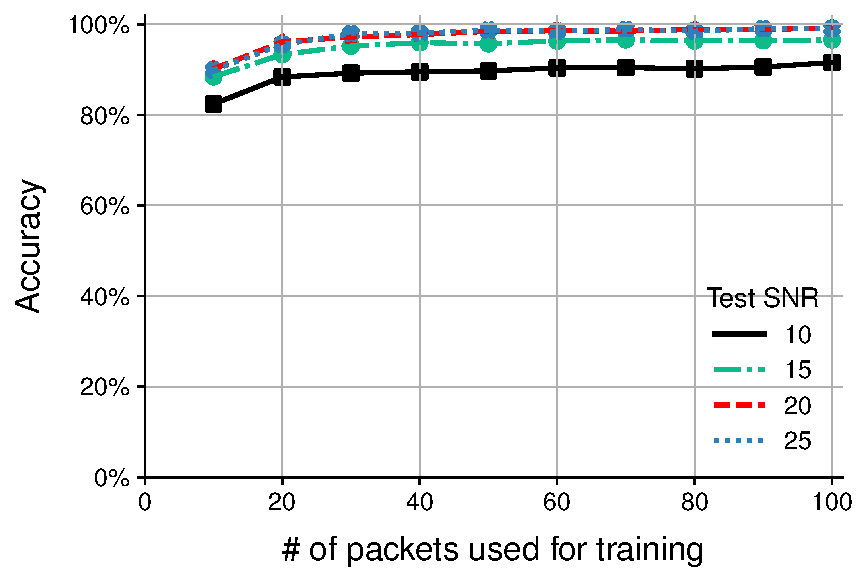
\includegraphics[width=\linewidth]{bletracking/plots/accuracy_esp_train2.pdf}
    \caption{Identification accuracy with different training sizes}
    \label{fig:esp_train}
\end{figure}
\end{comment}

We collected two datasets of BLE beacons from uncontrolled mobile devices.
%that happened to be transmitting BLE beacons at the time of data collection.
%
The first dataset was collected in public places that were likely to contain
many stationary BLE-enabled mobile devices, including: six coffee shops, a
university library, a food court. 
%
We set up a USRP N210 in each of these locations for approximately one hour,
and opportunistically collected BLE beacons. We observed hundreds of packets
from 162 unique devices across all the locations.
%
We used this dataset to evaluate the false positive (and false negative) rate of our BLE tracking toolkit.
%
The second dataset was collected in a facility where many unique devices passed 
briefly within range of our USRP N210. We observed dozens of packets from 647
unique devices over the course of 20 hours of data collection.
%
We used this dataset to evaluate the uniqueness of BLE physical-layer
fingerprints across a large number of devices.

%
%Even though we were analyzing captures from many real-world devices, we were
%careful to only capture and analyze BLE beacons and their corresponding
%physical-layer fingerprints.

\subsubsection*{Ethical Considerations}
Our data collection is completely passive, and we only capture BLE advertisement packets
(i.e., beacons) that devices already broadcast indiscriminately with the intention of being
received by any nearby device. Many of these packets originated from pervasive
BLE applications like contact tracing and device discovery. To ensure we only
capture BLE advertisement packets, we configured our SDR to only capture BLE
advertisement frequencies and mask off non-advertisement
channels~\cite{sparsdr}.  Furthermore, we ensure that in the decoding stage
only undirected advertising packets are passed on to the analysis phase.

The device fingerprints we produce as part of the analysis in this work cannot
be directly linked to individual people. Moreover, the BLE advertising packets 
from which we produce these fingerprints do not reveal any personally
identifiable information about the user of the transmitting device.  We only
performed full identification and tracking on 17
devices that we controlled.
According to our university's IRB office, this work does not qualify as
human subjects research.

%The question we intend to answer throught this section is \textit{Can we fingerprint the devices in field conditions? And are the device in-use such as phones, tablet, smart watches and so on distinguishable based on their RF fingerprints?}; Something that never has been addressed in prior RF fingerprinting work. 
\begin{comment}
In this section, we present insights about the distinguishability of the devices in the wild based on their hardware imperfections, by collecting a large dataset of BLE signals transmitted by commercial devices in use. We evaluate the feasibility of RF fingerprinting in the wild and elaborate upon the aforementioned challenges and limitations of RF fingerprinting using our field data.
\end{comment}

% \subsection{The choice of receiver}
% Our RF fingerprinting attack begins by capturing the BLE signals on the air using a Software Defined Radio (SDR). The first question that naturally rises is whether the choice of the SDR significantly affects the accuracy of our attack. In other words, \textit{can we use an inexpensive receiver such as LimeSDR-Mini to deploy such attack?} In fact the accuracy of our attack is dependent on the quality of the received signal and the extracted hardware imperfections. To show that the quality of the estimated hardware imperfections remains the same even if we capture with a less expensive receiver, we send packets from an iPhone device and capture the signal with both an USRP and a LimeSDR-Mini. Figure~\ref{fig:sdr_comp} demonstrates that the CFO values extracted from signals captured by these two receivers are very close to each other, indicating that using a cheaper receiver can be almost as good as an expensive one. Note that we measured the CFO difference between the receivers using a third device, and compensated for the difference in the receivers’ CFO by adding this CFO bias to the CFO captured by LimeSDR. As a result, as long as the SDR has a stable crystal that does not drift significantly over time, the choice of the SDR is not of a significant importance.

% \begin{figure}[t!]
%     \centering
%     \includegraphics[width = \linewidth]{plots/sdr_comparison_CFO.pdf}
%     \caption{CFO Comparison of two SDR receivers. After compensating for the CFO difference between the receivers, the measured CFO for the transmitter matches between two different SDRs}
%     \label{fig:sdr_comp}
% \end{figure}

\subsection*{Data Analysis}
 
We fingerprint and identify devices using our BLE tracking toolkit
described in Section~\ref{sec:methodology}.
%
We first determined how many packets from one device are needed in order to obtain the fingerprint and then identification.
%
To do this, we performed controlled experiments using off-the-shelf ESP32 devices at different SNR values and different number of packets observed.
%
The observation was that to establish a fingerprint the attacker need only 50 packets from the target BLE device, and this is sufficient even at low SNR values.
%
We also observed that once the fingerprint is established, a device can be identified or tracked by observing only 10 packets.
%
Considering that most mobile devices transmit several hundreds of BLE beacon packets per minute, an attacker doesn't need a lot of time to perform high-precision identification.

\if 0
We
found this threshold by performing a controlled experiment using 
20 ESP32 BLE chipsets. We tested in varying SNR conditions from 10
to 30~dB---exactly what an attacker would typically see in the field---to
see if the number of packets needed for fingerprinting and identification increases when 
beacons have poor SNR.
%which are from the same make and model, and captured their signals with a
%Software Defined Radio enables with SparSDR~\cite{sparsdr}.
Next, we identified each of the 20 devices using the algorithm
described in Section~\ref{sec:methodology2}. We split the captures used for
training and test as follows: 80\% of the beacons were used for training (i.e., fingerprinting), and
20\% for testing (i.e., identifying).  We trained with beacons at three SNR values:
$\{10,15,25\}$~dB. Then, we ran identification tests with beacons that had $\{10,15,25\}$~dB SNR
independently. We evaluated the identification accuracy of different training sizes with a test size of 10
packets. %Note that we are only looking for a conservative threshold.
%Since all packets from the same device don't have the exact same CFO and IQ
%imperfection because of estimation error due to noise and tolerance of the
%hardware, the question is how many packets we need to get from a device to
%build a robust and reliable profile for the device (fingerprinting stage), and
%having this profile for the device, how many packets we need to get from the
%device to be able to identify the device reliably in future (identification
%stage). 



\begin{figure}
    \centering
    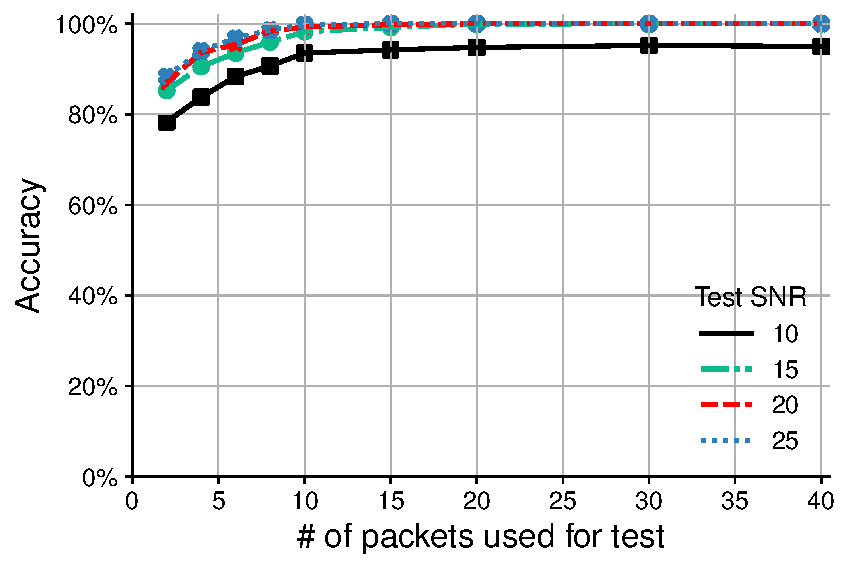
\includegraphics[width=\linewidth]{bletracking/plots/accuracy_esp_test2.pdf}
    \caption{Identification accuracy with different test sizes}
    \label{fig:esp_test}
\end{figure}


Figure~\ref{fig:esp_train} shows the accuracy of identifying the
devices compared to the number of training packets used for building the device fingerprints.
For all SNR values, having 50 packets for training is sufficient. Many BLE devices transmit
significantly more than 50 beacons a minute (Table~\ref{tab:beacon_rate});
therefore 
we estimate an attacker only needs to isolate
a mobile device for at most one minute to get enough packets to fingerprint it.


Figure~\ref{fig:esp_test} shows the accuracy of classifying the devices
compared to the number of packets used (the number of training packets is fixed
to 50 per device). 
%It is important to compare with the number of packets because obtaining more
%packets means that the target must be seen by the attacker for a longer period
%of time during the identification stage.
Across the tested SNRs, an attacker only needs 10 packets to accurately identify a device.
For the rest of the field study, we use 50 packets to fingerprint a device, and
10 packets to identify a device.
\fi
%For the evaluations presented in the next section, we did not need to filter
%out such MAC addresses.


%In fact, although we can have more than 99 percent accuracy with
%having more packets during the training and test, having 50 packets during the
%training and 10 packets during the test is sufficient to get more than 98
%percent accuracy for 15,20,25 dB SNR and more than 90 percent for 10 dB SNR.
%Therefore, in our field analysis, we will use 50 packets to fingerprint and
%build a profile for a device and 10 packets to identify it in future.



\subsection{False Positives and False Negatives}
\label{sec:results:field}


%To gain insights about the distinguishability of the devices in the wild, we collected BLE beacons from hundreds of devices in public areas such as five coffee shops and a library on January 2020 as described in previous section. 
%Even though we were analyzing captures from real-world devices, we were careful not to analyze the content of the packets we captured: we only analyzed the physical layer properties to perform our fingerprinting evaluation. 
%Moreover, we did not have any way of correlating a device's MAC address with the owner of the device and we only used these MAC addresses to compute a serial number in order to use as labels. 


%From the last subsections, we know that we roughly need 50 packets from a device to build a robust profile for the target device. We use 50 packets for cross-validation and the rest of the packets to evaluate the accuracy. As mentioned in the last subsection, using 10 packets to decide about the identity of the device seems sufficient. Hence, we first average the features for 10 packets and then calculate the closeness or distance to targets' fingerprinting model.

% TODO put back in somewhere
%This results in having a set of devices $\{1,2,3,...,162\}$. 

In the following experiments, we evaluate %the uniqueness of the stationary devices we
%observed in the field. Namely, we evaluate
the likelihood that our BLE tracking toolkit confuses a 
device that is not a target with a target (False Positive), and the likelihood
that it does not identify a target when it is present (False Negative).

Given the absence of ground truth of device identities in our dataset, we
relied upon the fact that BLE devices have stable MAC addresses for $\sim$15
minutes (after with they re-randomize the MAC address). Therefore, we used the
MAC as ground truth that multiple packets received were from the same device.
%
However, a device's MAC address can be randomized 
during our data collection, causing us to incorrectly treat the same
physical-layer fingerprint as two devices. We mitigated this problem by only considering devices that we 
observed during one contiguous period of time in each location where we did not
observe any new devices, nor any devices that appear to stop transmitting.
This filtering left us with 162 devices to use for our false positive and false negative evaluation.
%MAC addresses appeared, and (and thus appears to stop transmitting).

%First we select a threshold for the positive target identification based on the
%Mahalanobis distance metric in our classifier.

\begin{figure}[!h]
    \centering
    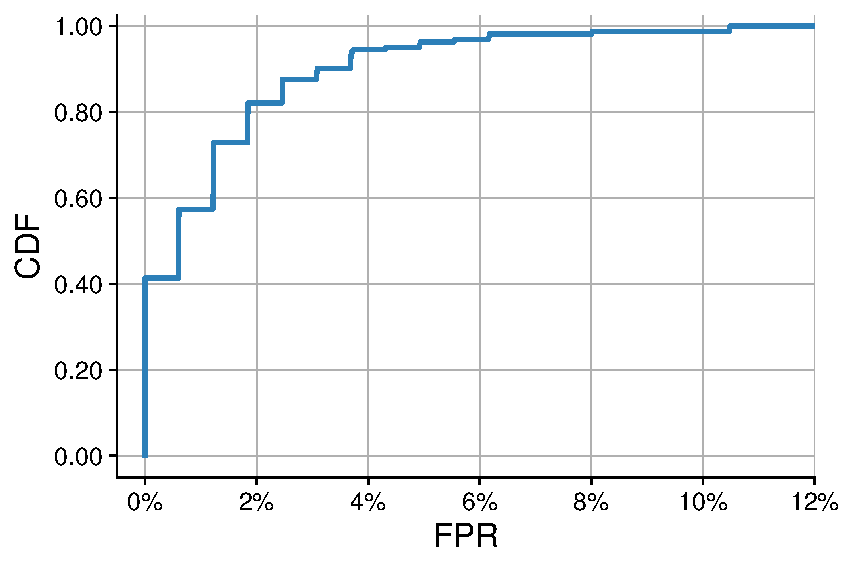
\includegraphics[width = 0.6\textwidth]{bletracking/plots/fpr_cdf2.pdf} 
    \caption{Dist. of FPR a device when comparing with all others}
    \label{fig:fpr_cdf}
\end{figure}



We consider every device (MAC address) $i \in \{1,2,3,...,162\}$ as a target,
and we train our classifier to find that device's fingerprint
(Section~\ref{sec:methodology2}).  Then, for each of the other devices, we run
the classifier to see if it identifies them as the target ($i$) device. If it
does, then that is considered a \emph{false positive}. The number of false
positives for target device $i$ divided by the total number of devices is the
False Positive Rate (FPR) for device $i$. Next, we fingerprint
each target $i$ and run the classifier to see if it fails to identify each device as
itself. Each instance of this is a \emph{false negative}. We repeat this process for all the 162 devices (each time one of
them is selected as the target), and divide the result by the total number of
devices to compute the total False Negative Rate (FNR). We observe our
classifier achieves a 2.5\% FNR across all 162 devices.



%Figure.~\ref{fig:fnr_cdf} demonstrates the CDF of FNR and
Figure~\ref{fig:fpr_cdf} shows the distribution of FPR for each of the 162 devices.
The median FPR of a device is only 0.62\%. Moreover, 40\%
of the devices were not confused with any other device (zero FPR), which implies many
devices seen in the field
have unique physical-layer fingerprints. Owning a device with unique 
imperfections makes someone particularly vulnerable to BLE tracking attacks. We also
observed
a small fraction of devices had an FPR as high as 10\%.
%for instance both CFO and IQ offset are small. The FPR for these
%.

%\begin{figure}
%    \centering
%    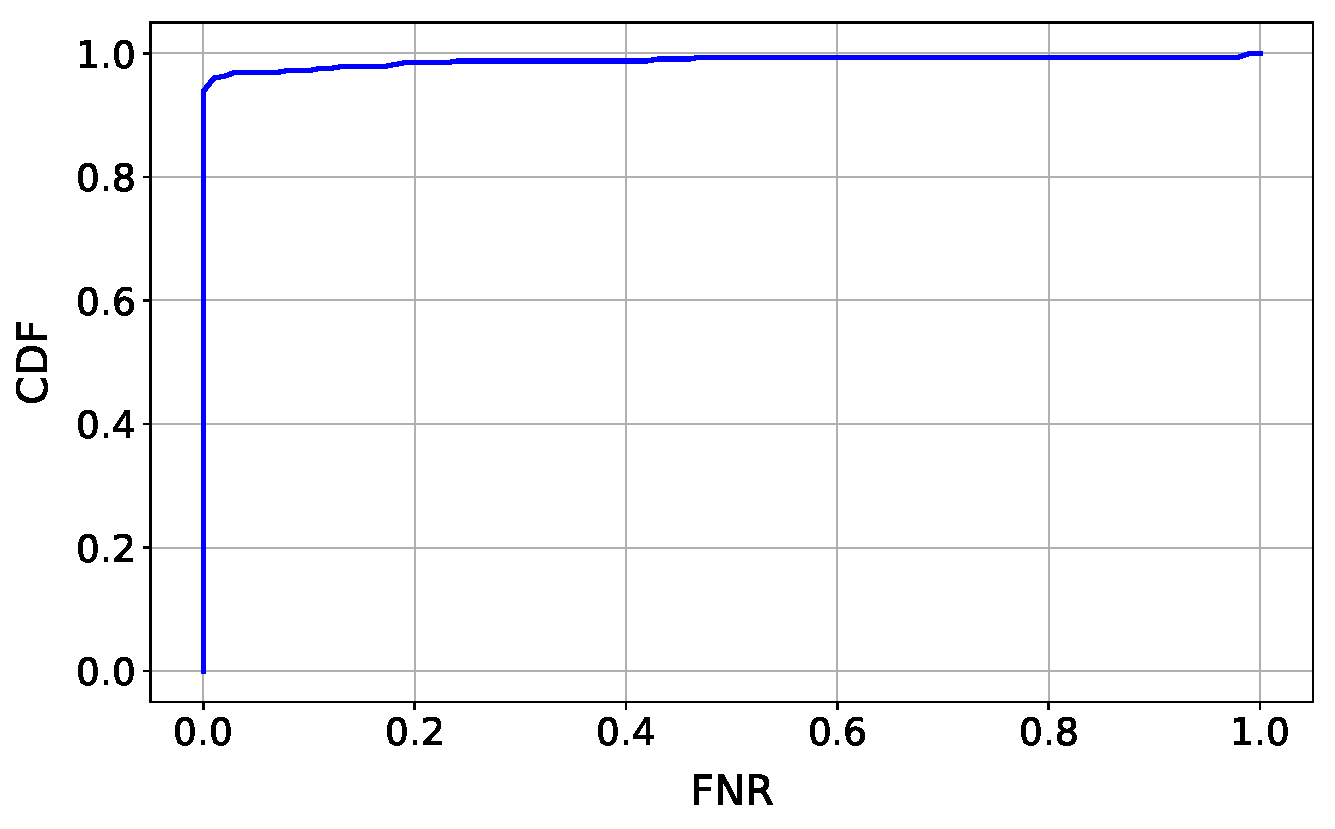
\includegraphics[width = \linewidth]{plots/fnr_cdf.pdf} 
%    \caption{CDF of FNR for the devices in the wild. Average FNR = 2.53\%. Median FNR = 0\%.}
%    \label{fig:fnr_cdf}
%\end{figure}

\if 0
\subsubsection{How imperfections contribute to identification}

Next, we evaluate how each of the imperfections contribute to
identification.  Table~\ref{tab:ablation} shows the FPR and FNR when using CFO,
\iq offset and \iq imbalance separately, and all together, by repeating a similar
experiment as we used to compare device manufacturers. CFO contributes the most
to identification, as it can have a wider range of values for different devices
compared to \iq imperfections. \iq imperfections alone have a much higher FPR, but 
they can resolve the confusion between devices with similar CFO.
This same phenomena is also visible our controlled lab experiments 
(Figure~\ref{fig:cfoiq}) where some devices have CFO values close to each other,
but their difference in \iq imperfection makes them distinguishable.
Also, recall that temperature can cause variation CFO while it does not have any notable impact on \iq
imperfections. As a result, \iq imperfections can help identify 
the target when it experiences temperature changes.
%Moreover,
%the FPR and FNR when only using CFO computed by our method, is better than FPR
%and FNR when use the baseline CFO computed by existing techniques described
%before. This significantly impacts the identification when we aim at
%identifying a device in the presence of a large set of other devices. In fact,
%as discussed in Section~\ref{sec:similarity} having a method to measure hardware
%imperfections with high precision is necessary to RF fingerprinting;
%otherwise the device with close fingerprints will be easily confused.

\begin{table}
    \centering
    \begin{tabular}{|l|c|c|}
    \hline
    Features used&FPR &FNR \\ \hline
    %Baseline CFO& 7.41\%& 3.49\%\\ 
    CFO only& 2.42\%& 2.45\%\\ 
    \iq offset only& 19.84\%& 2.39\%\\
    \iq imbalance only& 32.53\%& 1.52\%\\
    \textbf{All Features}& \textbf{1.21\%}& \textbf{2.53\%}\\ 
    \hline
    \end{tabular}
    \caption{Hardware imperfection-specific FPR and FNR.}
    \label{tab:ablation}
\end{table}
\fi

\subsubsection{Effect of device model}

Based on our controlled experiments (Section~\ref{sec:similarity}), we expect devices from the same manufacturer to be more
likely to be confused than devices of different manufacturers. To test this hypothesis, we used the technique
proposed in~\cite{celosia2020close} to distinguish Apple products in our dataset
from other devices. About 76\% (123 devices) in the dataset are Apple
products. The prominence of Apple products in the dataset is likely
because Apple enables their BLE-based device handoff service by default on many of their mobile products, including iPhones and Apple Watches.\footnote{We collected this dataset before COVID--19 contact tracing launched.}
%After COVID-19, while Apple product are still the majority of devices that beacon, we expect
%to see a much greater share of other devices (e.g. Android phones) as many
%contact tracing apps make the phones beacon BLE signals. 
\begin{table}[!h]
    \centering
    \captionsetup{justification=centering}
    \caption{Manufacturer-specific FPR and FNR.}
    \begin{tabular}{|l|c|c|}
    \hline
    Devices Compared & FPR & FNR \\ \hline
    Only Apple Products & 1.91\% & 2.40\%\\ 
    Only other Products & 1.15\% & 2.94\%\\ 
    Apple vs other & 0.15\% & --- \\ 
    \textbf{All Devices} & \textbf{1.21\%} & \textbf{2.53\%}\\ \hline
    \end{tabular}
    \label{tab:apple_table}
\end{table}



Table~\ref{tab:apple_table} shows the FPR and FNR of Apple products compared
with other products. As expected, the FPR when comparing Apple devices with other Apple devices (1.91\%) is greater than
the median FPR when comparing across all devices (0.62\%). Also, the FPR and FNR when comparing Apple products with 
other devices is close to zero.
% The reason
%could be that as one might expect, the hardware imperfections of the devices
This appears to confirm our hypothesis that devices from the same manufacturer are more likely to be similar to each other than devices from different manufactures.
%In fact, the controlled experiments in
%Section~\ref{sec:similarity} also showed that the hardware imperfection
%distributions of devices from the same make and model could be similar.
%Consequently, distinguishing devices from different models should be easier on
%average.

% \begin{table}[]
%     \begin{tabular}{|l|l|}
%     \hline
%      Device type&FPR \\ \hline
%      &  \\ \hline
%      &  \\ \hline
%      & \\ \hline
%     \end{tabular}
% \end{table}




\subsubsection{Effect of temperature} %{{{
\label{sec:temp}

%, for a high quality and a low quality crystal oscillator. The CFO of a low quality crystal with 8 minute cutting accuracy is significantly changed by temperature, resulting a drastic increase in FPR; while the same change in temperature has much less impact on a high quality crystal


%As mentioned earlier, most devices that beacon BLE packets, randomize their MAC address about every 15 minutes. Consequently, as the only way to label the devices in the wild is their MAC address, we at most have 15 minutes of data with the same label for most devices in the field. 

The temperature of the devices we observe in the field were unlikely to
experience significant temperature changes during the course of our data
collection. Therefore, we perform a model-based simulation to evaluate the
effect of temperature changes on FPR and FNR.  Recall that temperature changes
affect CFO because of the well-documented relationship between frequency drift
of crystal oscillators and their temperature (Section~\ref{sec:similarity}).
Using the curves in~\cite{temp_cfo1}, we calculate the change in CFO ($\Delta
f$) as temperature drifts further from the temperature baseline when the device
was fingerprinted ($\Delta T$~$^\circ C$). To ensure the target is not missed
even if the temperature changes are as large as $\Delta T$~$^\circ C$, we modified the
classifier to accept the device as the target even if the CFO of the device
is $\Delta f$ away from the fingerprinted CFO of the target. The consequence
of increasing the range of acceptable CFO values is that it increases the chance of
observing a device whose CFO falls in the acceptable range, resulting in an
increase in FPR.

\begin{figure}[!h]
    \centering
    \captionsetup{justification=centering}
    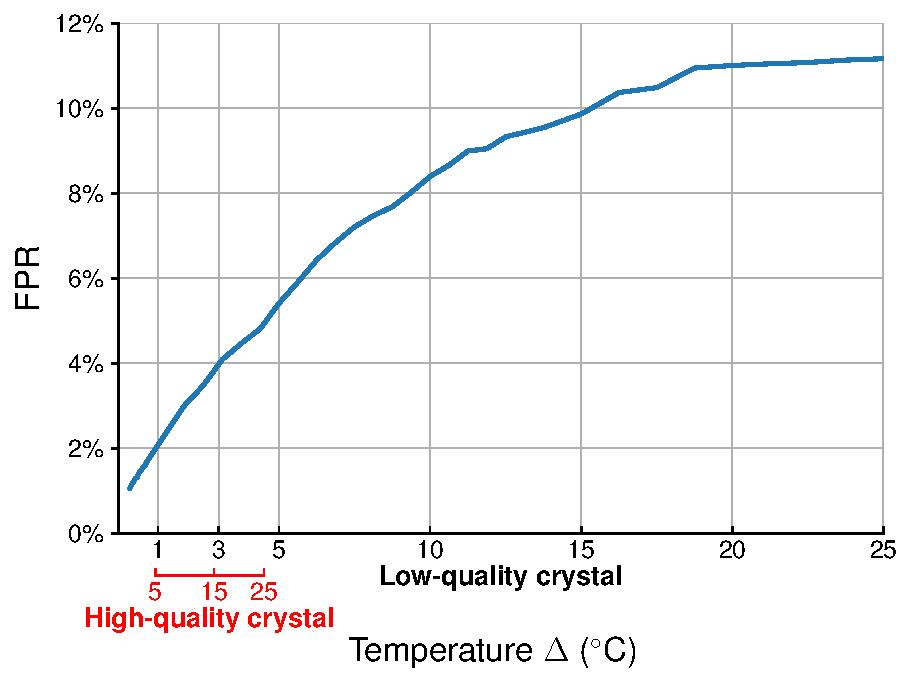
\includegraphics[width = 0.6\textwidth]{bletracking/plots/fpr_temp_thresh_new.pdf} 
    \caption{How oscillator temperature changes affect FPR.}
    \label{fig:fpr_temp}
\end{figure}


Figure~\ref{fig:fpr_temp} presents the FPR as the change in temperature increases. We
present the results for both high-quality and low-quality crystals (i.e.,
different cutting accuracies), as the type of crystal depends on the specific
device being targeted. Temperature change causes significantly less change in
CFO (and thus less increase in FPR) for high-quality crystals (0 minute cutting
accuracy) compared to low quality crystals (8 minute cutting accuracy). For
low-quality crystals, FPR increases rapidly as the temperature increases.  If
the change in temperature is too significant ($25^\circ C$), CFO 
becomes useless for identification: the FPR is the same as if we only used IQ offset
and IQ imbalance. In summary, temperature changes can severely limit an attacker's ability to track a target device.

%}}}

\subsection{Uniqueness of imperfections}

Recall that across the 162 devices observed in our first field evaluation dataset,
we found $\sim$40\% of the devices to be uniquely identifiable. % Therefore,
%hardware impairments like CFO and \iq offset and imbalance are unique
%enough to identity those devices. 
However, is natural to ask, is the same 
true at large scale? If the attacker were to observe several hundred devices
over multiple days, will we see a similar fraction of devices that are
uniquely identifiable?

To answer this question, we performed a larger-scale field data collection. We
placed an SDR at the exit of a room where \emph{hundreds of different
devices} passed by each day.  We recorded the Apple/Google COVID--19
Exposure Notification BLE beacons transmitted by those devices over the course of l0 hours on two days, separated by
one week to limit the number of duplicate devices. We computed the
mean CFO and mean \iq offset magnitude for each BLE MAC address
we observed in the beacons. The mean hardware imperfections are representative of the fingerprint of the BLE device. To reduce the chance that we observed the same
device with two or more different MAC addresses, we filtered out devices
which were observed for a duration longer than three minutes\footnote{Apple rotates addresses every 15~mins and Android every 10~mins.}. 


\begin{figure}[!h]
    \centering
    \captionsetup{justification=centering}
    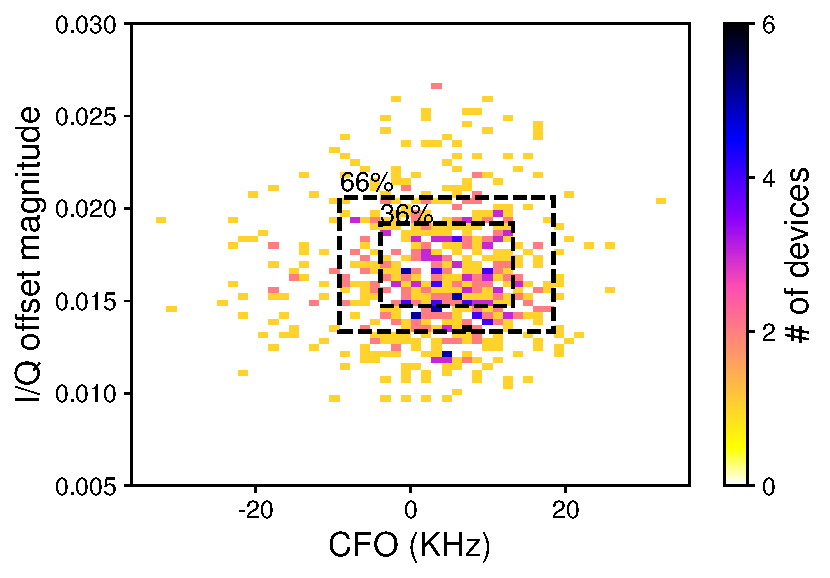
\includegraphics[width = 0.8\linewidth]{bletracking/plots/heatmap_hallway.pdf} 
    \caption{Histogram of imperfections across 647 BLE devices.}
    \label{fig:heatmap_hallway}
\end{figure}


We observed 647 unique MAC addresses 
across the two 20 hours of data collection.
Figure~\ref{fig:heatmap_hallway} shows the 2-Dimensional histogram of the fingerprints of these devices, namely their CFO and \iq offset magnitude.
%
The number of histogram bins were chosen so that the number of bins (2500) is significantly larger than the total BLE devices observed. Each bin represents a CFO range of $\sim$1.3 kHz, and an \iq offset magnitude range of 0.00516.
%
%hardware imperfections of these devices: their CFO and \iq offset magnitude.
Devices that fall in the same bin are considered to have indistinguishable hardware imperfections.
%
We also show the
bounds of the 2D histogram that cover 36\% ($\sim$$\sigma$) and
67\% ($\sim$$2\sigma$) of the devices ($\sigma$ because imperfections tend to be normally distributed). 

We found that 47.1\% (305) of the
devices were unique. This confirms that even
in a larger data set, $\sim$40\% of devices are uniquely distinguishable. We also observed that devices with overlaps did not
overlap with many other devices. For instance, 15\% (97) of the
devices had similar imperfections with only one other device. 

\iffalse
\subsection{Case Study 1: Temporal tracking of many targets}
\label{sec:results:case1}

Next, we conduct an experiment to evaluate how well our toolkit can track 17
controlled targets over time, in real world environments. 
%outside the set of devices collected in the wild.
These controlled targets are listed in Table~\ref{tab:targets}. Each target is isolated in an office to capture 50 packets to train the classifier with its fingerprint.
%and 50 packets for evaluation. These
%targets are profiled using the training and evaluation data and the profile of
%each device is stored and used in the rest of the study to compute FNR and FPR. 
 
\subsubsection*{False Negative dataset} Between 2--7 days after we
fingerprinted the targets, we individually took them to a different location,
and we captured their packets using a USRP N210 sniffer placed
10~ft away from the targets. We did not strictly force the targets to have the
same temperature in the office and food court, but both environments were
air-conditioned indoor buildings and there was nominal activity on the targets.

\subsubsection*{False Positive dataset} We evaluated the FPR for these targets
using a trace from a coffee shop from our field datasets, because we knew the
17 controlled devices were not present during that experiment.

\subsubsection*{Temporal FNR and FPR} We calculate the FNR and FPR over time,
in each 10 second interval of the captures. In each time interval, we provide 10
packets from each MAC address to the classifier to determine if it matches any
of the 17 targets' fingerprints. The FNR is the fraction of intervals where the
target was present, but was not identified, and the FPR is the fraction of
intervals where the target was not present, but was mistakenly identified.

\begin{figure}[t!]
    \centering
    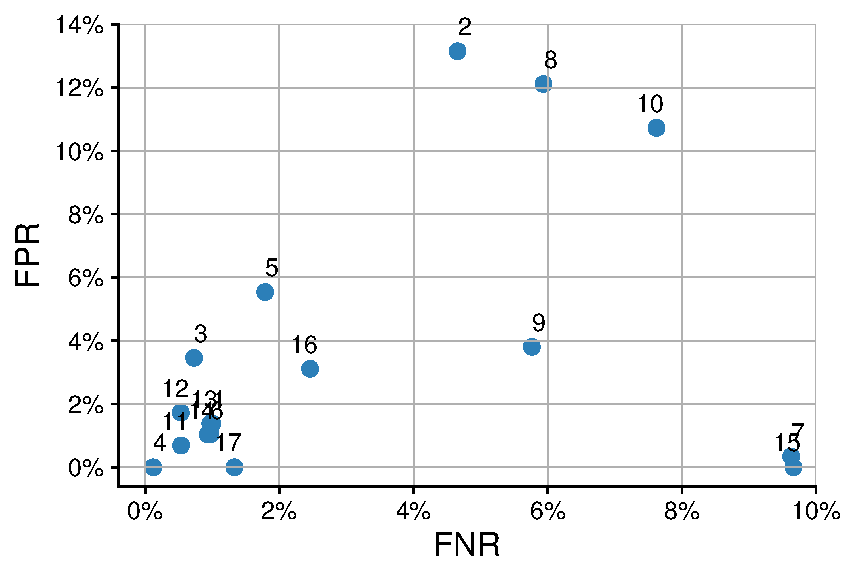
\includegraphics[width = \linewidth]{bletracking/plots/fpr_fnr2.pdf} 
    \caption{FNR--FPR for 17 controlled targets.}
    \label{fig:fpr_fnr}
\end{figure}

\begin{table}
    \centering
    \begin{tabular}{|l|l|l|}
    \hline
    \#: Device&\#: Device&\#: Device\\ \hline
    1: iPhone 10&7: iPhone 10&13: MacBook Pro\\ 
    2: iPhone 8&8: iWatch&14: Thinkpad\\ 
    3: iPhone 11&9: iPhone 10&15: AirPod\\ 
    4: Bose Headset&10: iPhone 8&16: Pixel 2\\ 
    5: iWatch&11: iPhone 10&17: Pixel 5\\ 
    6: iPhone 8&12: iWatch& \\ \hline
    \end{tabular}
    \caption{17 target devices used for this experiment and their label numbers that are used in Figures 16 and 17.}
    \label{tab:targets}
\end{table}

\subsubsection*{Results}

Figure~\ref{fig:fpr_fnr} shows the average FNR and FPR for these 17 targets. The average FNR of these controlled targets is 3.21\% and the average FPR is 3.5\%. Although there are a few devices with high FNR and FPR, most devices have distinguishable hardware imperfections, resulting in low FNR and FPR.

Figure~\ref{fig:fpr_time} shows the temporal patterns of false positive
occurrences for each of the 17 targets in one of the field traces. Each time
there is a bump in a device's horizontal line, it means that at least one
device was mistakenly identified as being the target during that time interval.
We observe that false positives are sometimes short-lived, but often they last
for longer than one 10-second interval, possibly indicating a device with
similar hardware imperfections came within range of the
sniffer. 

%In some cases, a MAC address is falsely detected as our target but after a while it dissapears and a new MAC address causes the false positive occurance, possibly because the device has changed its MAC address and the new confused MAC address is the same device that was confused before which has changed its MAC address. 
%There also exists a very few false positive occurrences that last for a few seconds. This is because sometimes we did not get enough packets from a device in 10 seconds and the hardware imperfections of the very few noisy packets looked like our target. However, after getting more packets from that device, it turns out we were wrong and false positive is resolved in the next time slots. Finally, its worth mentioning that on average, we saw 18 unique MAC addresses in each 10 seconds and overall we saw 259 unique MAC addresses during this 48 minute capture at a coffee shop.



\begin{figure}[t!]
    \centering
    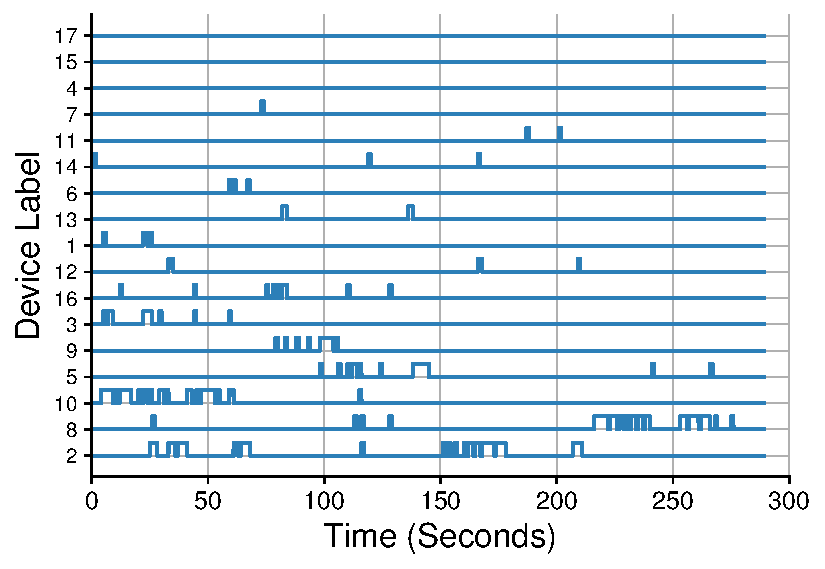
\includegraphics[width = \linewidth]{bletracking/plots/fpr_time_10sec_sort2.pdf} 
    \caption{FPR occurrences over time for each of the 17 targets.}
    \label{fig:fpr_time}
\end{figure}










\subsection{Case Study 2: Tracking a person}
\label{sec:results:case2}

%\begin{figure}[t!]
%    \centering
%    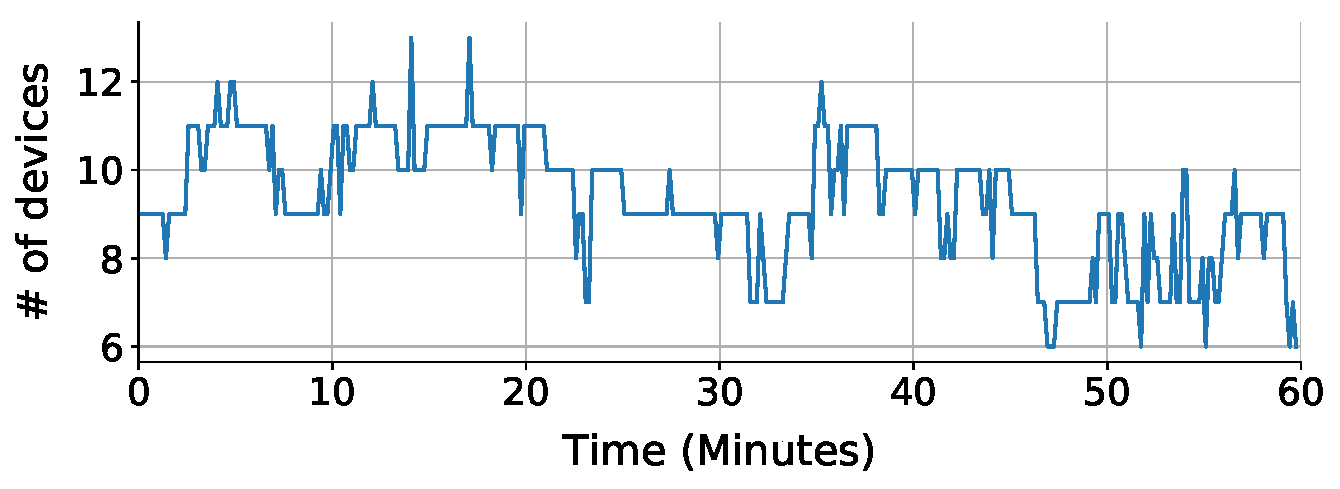
\includegraphics[width = \linewidth]{plots/case_study_iphone_devno.pdf} 
%    \caption{Number of unique MAC addresses observed over time duuring the experiment of tracking iPhone}
%    \label{fig:iphone_no}
%\end{figure}
%
%
%\begin{figure}[t!]
%    \centering
%    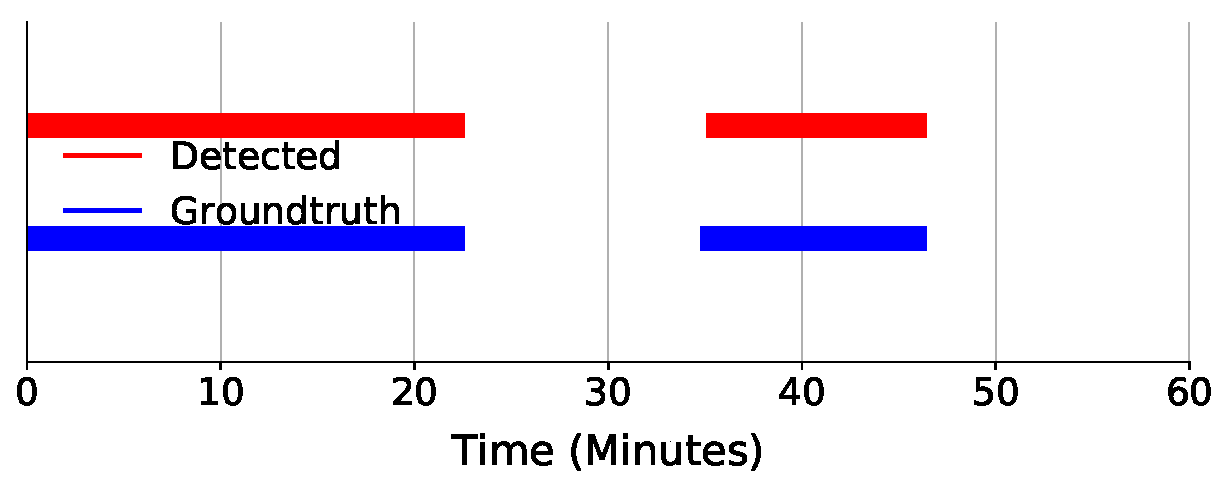
\includegraphics[width = \linewidth]{plots/case_study_iphone.pdf} 
%    \caption{The blue bar represents the time that the iPhone target was present and the red bar represents the time that our algorithm detected the presence of the iPhone}
%    \label{fig:iphone}
%\end{figure}



Finally, we describe an end-to-end tracking attack we executed on a controlled
target (a volunteer who uses an iPhone).
%
The attacker first carries their SDR sniffer close to the target device to
obtain the device's physical-layer fingerprint. Simultaneously, the attacker
scans for nearby BLE devices using a commonly available BLE scanner phone app,
and they record the MAC address of the BLE device with the highest observed
signal strength, which is the nearest device (i.e., the target's phone). Later,
they use this MAC address to pick out the target device's packets from the raw
sniffer capture. Then, they feed these packets into the BLE tracking toolkit to
train its classifier with the target device's fingerprint.

After creating the fingerprint, the attacker tracks their target by placing an
SDR and laptop close to their target's home. The attacker can determine when the target is
home by observing when the classifier running on the laptop indicates the packets received by the SDR match the target device's fingerprint.
%
The attacker tracks their target for one hour, during which the target walks
inside and outside the house 2 times. Figure~\ref{fig:android_no} shows the
number of unique MAC addresses observed every ten seconds during this hour.
There are approximately 30 other devices nearby that could be confused with the target.

%\noteby{NB}{5 - Add information about how the attack was carried out}

The blue bar shown in Figure~\ref{fig:android} shows the ground truth of when
the person was inside the house during this hour. The attacker's identification
toolkit runs once every 10 seconds, and the red bar shows the time durations
during which the tracking toolkit thinks the person was present. The bars
perfectly match except for immediately prior to minute 10, where the toolkit
falsely detects the presence of the target for 50 seconds, even though it had
not yet actually returned.

%Next, we repeat the same experiment when the volunteer is carrying a pixel 5 phone. This time, we also reduce the power level threshold that our sniffer captures the signals. As shown in Figure~\ref{fig:android_no}, we capture signals from more devices in a wider range from the sniffer. Figure~\ref{fig:android} shows the groundtruth time when the person was present and the time which [name] detected the presence of the person. This time, we mistakenly think our target was present for about 50 seconds while they were not. This confusion happened for a single MAC address and was resolved when the MAC address disappeared. As we have increased the range that our receiver can receive, this device most likely belonged to a person passing by around the house. In both scenarios, we demonstrated that one can deploy the RF fingerprinting attack in a real-world scenario with high accuracy, threatening the privacy of the device owner.
\fi
\begin{comment}
\subsection{Case Study 3: Uniqueness of BLE devices at scale}
\label{sec:results:case3}

\begin{figure}[t!]
    \centering
    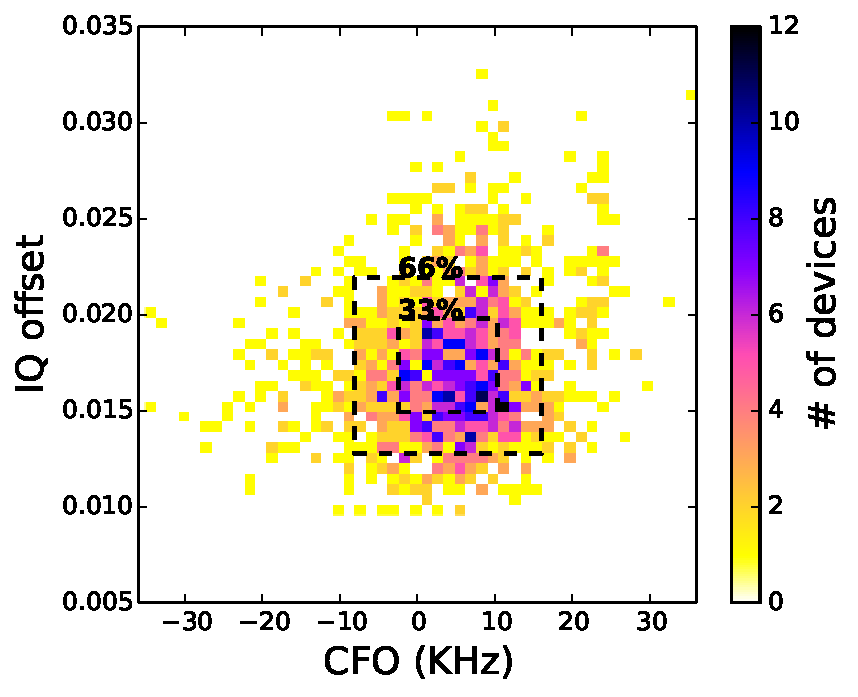
\includegraphics[width = \linewidth]{plots/door_2dhistogram.pdf} 
    \caption{Distribution of CFO, \iq offset for devices passing through common entryway}
    \label{fig:2dhistogram}
\end{figure}
In Section~\ref{sec:results:field} we analyzed the 162 devices observed at coffee shops.
%
These provided a good snapshot of uniqueness of BLE hardware impairments of smartphones in the wild.
%
However, the number of devices observed was small, and therefore we didn't know what would happen if the number of devices were to scale
To understand 
\end{comment}





%%!TEX root = paper.tex
\section{Discussion}
\label{sec:discussion}

\subsection{Why we think we are not missing skimmers} %{{{

Throughout the course of this study, we have been in direct communication with government officials from numerous states
responsible for the removal of skimmers, and have developed a working relationship wherein we are notified any time
a new breed of skimmer appears which is currently undetected by the Bluetana application.
%
Thus, our ability to detect skimmers depends upon the current level of investigation performed by government officials;
%
if a skimmer using a new OUI previously unflagged were to be discovered at a gas station by any of the 40+
investigators, it is likely we would be notified.
%
In fact, this has already occurred.

This lends confidence to our measurements and analysis \textit{at the current point in time}.
%
In the coming years, criminals may make a shift to using other technologies, i.e. radio, to retrieve data from
skimmers.
%
Now we will discuss ...
%}}}

\subsection{Countermeasures} %{{{

\subsubsection{EMV}
\label{sec:discussion:emv}

Credit card companies will soon require upgrading magstripe terminals to to EMV
chip technology \todo{cite}.
%
Although there are fewer vulnerabilities with EMV cards, namely the attack the
exposed reader cabling attack vector, that brought on internal skimmers
\todo{cite}.
%
There are obvious concerns on if this is realistic, as gas stations operators
were required to upgrade fuel dispensers to the new EMV-based card readers by
2018, but the deadline was extended but the large number of gas stations makes
it prohibitively expensive to do so, and therefore the deadline was extended.

Already, criminals have productised EMV versions of internal skimmers, called
deep-insert skimmers, or ``shimmers''.
%
Deep-insert skimmers bear striking resemblance to the magstripe internal
skimmers.
%
The reason is, both magstripe and chip card readers transfer card information
over a digital serial bus.
%
However, instead of tapping into the serial signal at the exposed cabling, EMV
skimmers are inserted fully into the cardslot.
%
Newer EMV chip cards obviate the need for an analog decoder by directly
providing the digital serial interface.
%
If you tap into an EMV signal you can still produce a mag-stripe card and use
it somewhere else \todo{cite}.

% \begin{figure}
% \centering
% 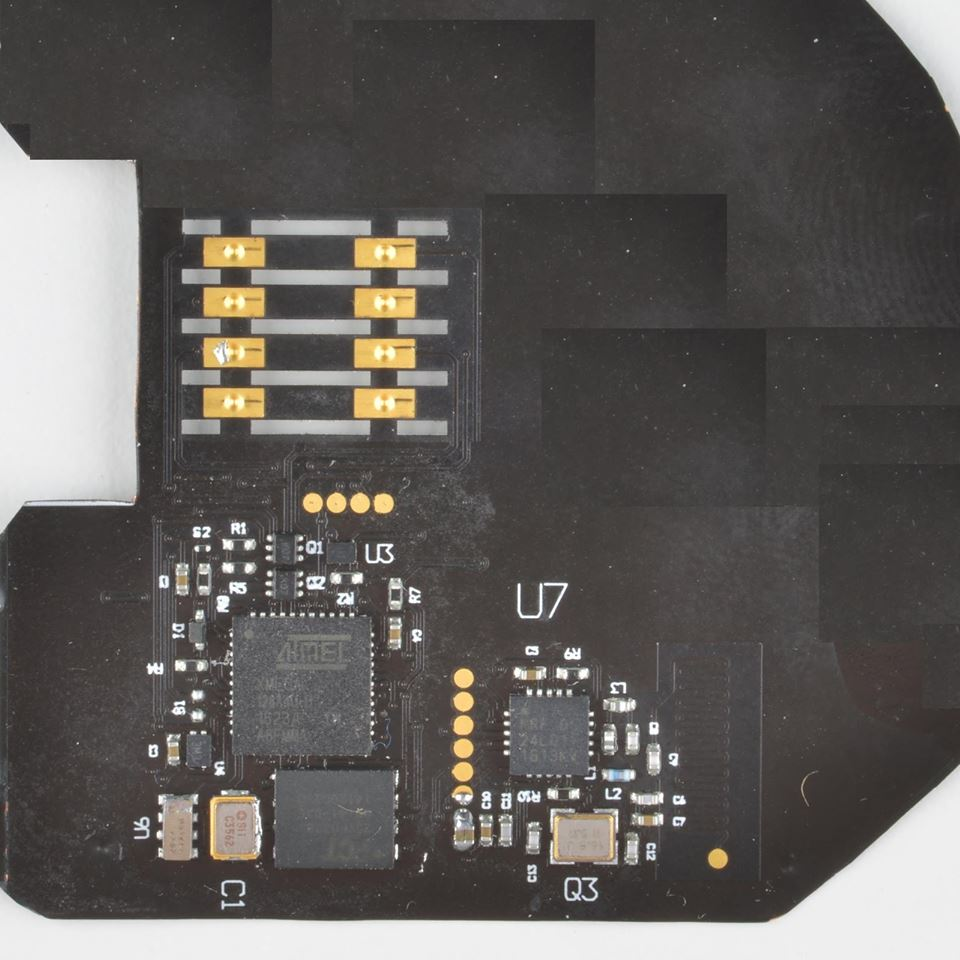
\includegraphics[width=0.5\linewidth]{fig/deep-insert}\\
% \small{Image source: gas-pump-skimmer.com}
% \caption{
% \label{fig:deep-insert}
% A ``Deep-insert'' EMV chip skimmer with wireless (Bluetooth Low-Energy) exfiltration capability.
% }
% \end{figure}

Figure~\ref{fig:deep-insert} shows an example of a deep insert skimmer that
demonstrates they are just a new version of internal skimmers in that they
passively capture card information, and they have a wireless interface for
exfiltration.

% https://link.springer.com/chapter/10.1007/978-3-642-04904-0_7
%}}}

\if 0 %{{{

\subsubsection{Physical security}
\label{sec:phys-security}

Although it would appear that card security was not a priority in the design of
fuel dispensers, the PoS circuit encrypts all payment information in transit to
the central payment processing unit in the gas station.
%
Rather, the security measures did not protect against tiny embedded system
could be installed inside the enclosure and exfiltrate the data wirelessly.
%
This is also indicated by the poor physical security in enclosure designs that
could have stopped criminals from gaining access into the internal circuitry.
%
Details about the physical security vulnerabilities of fuel dispensers are
discussed in Section~\ref{sec:phys-security}. 

\begin{figure}
\centering
\includegraphics[width=\linewidth]{fig/tamperseal-pump.jpg}
\textbf{Multiple tamper-evident seals on a dispenser.}\\
\vspace{0.2in}
\fbox{\includegraphics[width=\linewidth]{fig/tamperseal.png}}\\
\textbf{Identical seals can be purchased online.}
\caption{
\label{fig:tamperseal}
Criminals can easily replace voided seals.
}
\end{figure}

\paragraph{Tamper-evident seals}
%
Criminals also have to bypass any tamper-evident seals that the station owner
attaches to the dispensers.
%
In theory tamper-evident seals should deter criminals from installing skimmers.
%
However the significant effort required to maintain tamper-evident seals at
fuel stations makes them cumbersome to use.
%
An attendant must replace the seals every time the dispenser is inspected and
serviced.
%
Interestingly, some stations even install multiple seals with the intention of 
improving security, however this only makes it more difficult to check
if a criminal has replaced the seal with a new seal that has a different serial
number (Figure~\ref{fig:tamperseal}).
%
As such, we have found many tamper evident seals at gas stations are cut or
activated.
%
As further evidence of how ineffective security seals are, replacement security
seals were found in the possession of criminals that were arrested while they
were installing a skimmer~\cite{texas_criminal_security_seal}.





As described in the sections above, Bluetana has been and continues to be an effective weapon in the law enforcement fight against skimmers in the wild. Our methodology essentially uses characteristics of commodity Bluetooth devices in skimmers to be able to detect them. As details of our methodology become public, criminals will try to adapt to prevent skimmer detection. Based on knowledge gathered over the course of our research, in this section we try and analyze possible modifications that can be made to current skimmers to make detection more challenging, and whether Bluetana measures up. We also try to present this section as a lookahead of how the skimmer landscape might evolve in the future and thus present this as a point of reference for future work in the area.

Q : Why dont the criminals simply migrate to a longer range wireless communication mechanism like cellular?

A : By the looks of it, for a skimmer application cellular seems to be a good fit. Criminals are saved from the burden of having to drive to gas stations to collect data, thus putting more distance between them and the scene of the crime. Cellular radios however add an extra cost of requiring to purchase a SIM card with an active cellular plan. Cellular radios themselves are in general costlier than commodity Bluetooth modules and thus overall skimmer cost goes up. Addtionally, when recovered, presence of an active cellular connection can give law enforcement a much easier investigative route to pursue the criminals. Consequently, added cost and higher risk make cellular radios less likely to be used for skimmers in the future

Q : Well if not cellular, what about other wireless radios

Q : Gas pumps are now migrating to chip based readers which they are secure, so this wont be a problem in the long run, right ?

A : Not so much. Most current migration is cosmetic. Replacing entire CRIND tray mechanism or buying new machines is costly, and so current chip based modular replacements, simply read data from the cards but transmit to the backend POS in the clear. Even if we consider the case that new models of pumps based on chip readers are installed, chip based EMV mechanism has been found to be vulnerable to replay attacks because of weak RNG [cite IEEE paper]. In fact, ingenous skimmers already exist in the market that take into account these weaknesses and are able to bypass SDA, DDA and CDA to create a data dump that can be used to create perfect clones [cite website for skimmer]. However, the idea of using wireless radios to ease in the data collection and reduce chances of getting caught, are still valid and will hold. Hence focussing on this interface as a means for detection will continue to stay valid. Case in point, the chip skimmer also has a Bluetooth radio onboard

Q : A major component of your paper has been the idea of crowdsourcing, and yet you only collected data for the survey using a few individuals?

A : The idea of multiple individuals using the toolkit to detect skimmers in a large geographic area does remain valid. During development of this toolkit, we were concerned about details of our method leaking to criminals, and thus it was important to keep the circle of trusted individuals small, and thats why we the authors took to scanning the gas stations ourselves. We are in conversation with multiple state level Weights and Measures and local PDs, and will soon have large scale crowdsourcing in place. However, the fact that only a few individuals scanning for skimmers at gas stations were able to recover 10 odd skimmers, does tend to lend credence to the argument that with a large scale deployment, we will have signifantly greater capture rates

\begin{enumerate}
\item  Unnamed Devices are a limitation
\item   We use the MAC address, other metrics in that case
\item   Method in field relies more on the hitlist
\item     Hitlist can be comprehensive
\item     Using data from police recovery, as well scraping of
    websites like alibaba, sparkfun, digifruit, ebay, ...
\item    	      Incremental; if a new device shows up and
	     we are notified, we can rerun metric analysis to
	     find the new hitlist devices
\item	      method is extendable
\item What about randomized MAC addreses / smarter skimmer
\item   Full randomization, the criminal must rely on the device name
  to recover the device, since the person that is extracting the
  data is not the same as the one that implanted. Crims generally
  use mules, according to law enforcement agencies.
\item   Now, there can be a limited randomization, in which you use
  a pool of MAC addresses
\item     This is more sophisticated, and damages our methodology, the
    mitigations for this are more complicated but come in one of
    two forms: either persistent monitoring devices at each gas station
    or an even larger crowd sourced approach, wherein you get enough coverage
    of each gas station to determine persistence
\item        This is more difficult to detect. You could flag based upon whether
       the MAC address device is abnormal compared to a baseline for other
       gas stations: if you see a thermostat, it is bad.
\item        But even apple uses 47 bits of randomization, trampling upon other
       manufacturers, so how do you tell this is not another consumer
       electronic, or that the criminal is not masquerading as a common
       bluetooth device, i.e. a Tile?
\item  So consider the case of a smart criminal (i.e. one of the authors of this
paper) designing a skimmer. They would randomize the fingerprint so that
it looks like one of 255 tiles.
\item    In a largescale crowdsourced approach, you might, in the best case,
   have someone come by and scan the gas station every 3 hours. Using our
   methodology, this would not flag odd name, bad MAC, seen twice ... 
\item    There is still a possibility! For each gas station, record the geoloc
   of each of the pumps. For each gas station, check the rssi of the devices
   scanned, and see get a high confidence localization inside the pump. From
   multiple datapoints, you should be able to determine whether the bluetooth
   device is inside of a pump, and there are no bluetooth devices commonly found
   inside pumps.
\item    and you can't spoof RSSI. It is approximate, and depends on the phone/reciever
\item    Since each phone has a subjective perspective, to get the ground truth, you
   would localize to a centroid for each observer, and then combine these centroids
   to localize the skimmer.
\item    Thus, even if criminals were not dumb, we could find them.
\end{enumerate}
\fi

%}}}

%!TEX root = paper.tex
\section{Countermeasures}
\label{sec:countermeasures}

\begin{figure}[t!]
    \centering
    \includegraphics[width = \linewidth]{bletracking/plots/case_study_android_devno2.pdf} 
    \caption{Number of unique MAC addresses observed over time while tracking the target.}
    \label{fig:android_no}
\end{figure}

BLE location tracking based on hardware impairments cannot be defended against by simple software/firmware update
mechanisms. These manufacturing variation based properties
are baked into the RF signal chain.
%; as long as the device transmits the signal will have CFO and I/Q offset and imbalance.

One possible defense against this attack requires us to rethink the design of a BLE chipset's signal chain.
%
We envision adding a random time-varying extra frequency offset the crystal oscillator.
%
This would cause the CFO measured at the receiver to also be time-varying and unpredictable.
%
Fortunately, since BLE has a large CFO tolerance (150 kHz~\cite{btcorespec}), an extra frequency shift will not impact packet decoding.
%
%However, our attacker who relies on a stable CFO to track the target, will no longer be able to utilize these hardware impairments as a reliable identifier.

We also envision another defense that does not require hardware modification.
%
In Section~\ref{sec:challenges:temperature} we observed that CFO changes significantly when a device's internal components heat up and cool down.
%
Internal component temperature depends on the workload running on the phone: a time-varying workload can result in a time-varying CFO.
%
We envision a defense in which a background process runs a computation, and keeps randomly changing the computation in line with the MAC address changes.
%
Unfortunately, a constantly changing workload can result in a constantly changing battery consumption.
%
Worse still, if the device temperature remains constantly elevated, the battery life also decreases over time~\cite{fireinyourhands}.

\begin{comment}
We envision the following possible countermeasures to defend against the location tracking attack.
%
Since CFO is the major contributor to BLE device identification (Section~\ref{sec:results:field}), we focus our defenses on manipulating this property only.
%



\subsection{Modifying the crystal oscillator circuit}
\noteby{NB}{
As we have seen, for any BLE chipset the CFO imperfection arises in the crystal oscillator circuit of the BLE radio.
%
The mobile device is identifiable because the CFO imperfection is unique to any BLE radio.
%
Therefore, we can envision the design of a new crystal oscillator circuit that adds a fake CFO beyond the inherent CFO imperfection
}

\subsubsection*{Limitations}
\noteby{NB}{
Implementing something like this would require a complete redesign of the BLE radio chipsets, which is time-consuming and costly.
%
Additionally, this solution only benefits future BLE radios. 
%
The millions of phones already in operation will still use the unmodified BLE radios and will remain vulnerable to the tracking attack.
}
\end{comment}

%!TEX root = paper.tex
\section{Related Work}
\label{sec:relatedwork}
%\todo{Move related work top}
\subsection*{BLE MAC-Layer Fingerprinting}
%
At its most basic level, BLE's design frustrates MAC-layer fingerprinting.
%
Although BLE advertisements contain a full 6-byte MAC address that is unique to the
advertising device, the BLE protocol also has built-in cryptographic MAC randomization.
%
Fortunately, prior work found (and we confirmed) that mobile devices are
properly implementing BLE's MAC address randomization~\cite{Iphonetracking_becker,MACRandomizationfail_Martin}.
%
Namely, they found devices are following the BLE specification and periodically
(every 10--15 minutes) randomizing their MAC addresses~\cite{bluetoothprivacy}.
%

However, several papers have performed privacy attacks by deriving identifiers from the packet contents of beacons that were not reset properly after the MAC was
randomized, for both WiFi~\cite{sn1,MACRandomizationfail_Martin} and BLE~\cite{ryanble,spill2007bluesniff,Iphonetracking_becker,HandoffMartin,celosia2020close} radios.
%
However, all of these attacks fall short as they either require the receiver to continuously listen to beacons from the target devices, or fundamentally rely on identifiers that can easily be removed through simple software updates.
%
This limits the attacker's ability as they must persistently follow a target to track it.
%
Thus, link layer techniques don't provide persistent identifiers that can be utilized for long term tracking of devices.

\vspace{0.5em}

\subsection*{Physical-layer Fingerprinting}


RF fingerprinting using hardware impairments is a well studied field.
%
Researchers have analyzed various hardware impairment based signal properties such as CFO, \iq offset/imbalance, signal transients and others~\cite{Brik_radiometric,vohuuusrp,Intrusion_hall,deviceID_kose,suskitransient,roguewifi_liu,oscillator_azamehr}, and leveraged various statistical methods, and in recent times deep learning approaches~\cite{gopalakrishnan2019robust,denoising_yu,deeplearning_merchant} to fingerprint these properties. For instance, the transient portion of the signal has been proposed as a unique signature to 
classify different wireless devices~\cite{extraction_rehman, transientID_danev} even Bluetooth
signals~\cite{transientBT_Hall}. However, the transient portion of BLE and Bluetooth signals
is only about 2 microseconds and contains insufficient information to uniquely identify 
a device among tens of devices. Modulation-shape features have also been explored for RF
fingerprinting devices such as RFID transponders~\cite{rfidphysical_danev}. However, 
the Gaussian shape in GFSK modulation of BLE signals is generated digitally in most 
personal electronic devices such as phones, and thus, cannot be used as a unique fingerprint.
In the WiFi literature, CFO and \iq imperfections (\iq origin offset and \iq imbalance) are 
two well recognized features which have been shown to be the most separable features for 
WiFi fingerprinting~\cite{Brik_radiometric}. 

BLE hardware in mobile devices are similar in architecture and suffer from the same hardware impairments as WiFi radios.
%
Despite that, other than a few efforts at coarse CFO extraction utilizing specialized hardware (CC2400)~\cite{cvtracksun,blueshieldjain}, there exists limited work in RF fingerprinting of these BLE chipsets. 
%
This is primarily because the techniques to extract these properties rely upon the presence of long known sequence of bits and pilots, a convenience not provided in simple BLE transmissions.
%
Even if the WiFi techniques were utilized for BLE signals, they would yield coarse estimates of these persistent identifiers, which are not particularly useful when fingerprinting a large amount of devices.
%
Furthermore, to be able to utilize any RF fingerprinting technique as a privacy attack, we need to have evidence that it works in real world settings. 
%
Unfortunately, all prior work in RF fingerprinting has been performed in controlled environmental settings with a defined set of devices. 
%
We design a technique to extract the hardware impairments such as CFO and \iq offset from BLE signals at a fine granularity. We were then able to collect a massive dataset of BLE devices in the wild and analyze their RF fingerprints to evaluate the potentials and limitations of the physical-layer fingerprinting privacy attack in the wild. We also demonstrated the feasibility of a location privacy (tracking) attack utilizing these physical-layer parameters in a realistic scenario.








%!TEX root = paper.tex
\section{Conclusion}
\label{sec:conclusion}

In this work, we evaluated the feasibility of physical-layer tracking attacks
on BLE-enabled mobile devices. We found that many popular mobile devices are
essentially operating as tracking beacons for their users, transmitting
hundreds of BLE beacons per second. We discovered that it is indeed feasible to
get fingerprints of the transmitters of BLE devices, even though their signal
modulation does not allow for discovering of these imperfections at decoding
time. We developed a tool that automates recovering these features in
transmitted packets.

Then, we used this tool to determine what challenges an attacker would face in
using BLE to track a target in the wild. We found that attackers can use
low-cost SDRs to capture physical-layer fingerprints, but those identities may
not be easy to capture due to differences in devices' transmission power, they
may not be stable due to temperate variations, and they may be similar to other
devices of the same make and model. Or, they may not even have certain
identifying features if they are developed with low power radio architectures.
By evaluating the practicality of this attack in the field, particularly in
busy settings such as coffee shops, we found that certain devices have unique
fingerprints, and therefore are particularly vulnerable to tracking attacks,
others have common fingerprints, they will often be misidentified. Overall, we
found that BLE does present a location tracking threat for mobile devices.
However, an attackers ability to track a particular target is essentially a
matter of luck.

\begin{comment}
In this work, we have built an RF-identification attack, which provides the ability to identify the presence of a user or multiple users, even in the wild via their smart portable electronic devices which are continously leaking their privacy through frequent BLE transmissions. In addition, fundamental differences in some BLE architectures compared with other wireless technologies was presented and novel techniques for fingerprinting and identifying all kinds of existing BLE architecture were proposed for the first time. We evaluated our attack in uncontrolled noisy environments in the wild where exists a large number of random devices, demonstrating the practicality and feasibility of our attack.
We believe the feasibility of this attack in the wild, signifies the importance of implementing physical layer security techniques. We hope our work encourages chip vendors to hide physical layer signatures in their future designs and enable secure RF front-end design for wireless communication.
\end{comment}
\begin{comment}
In this work, we have built an RF-identification attack, which provides ability to identify the presence of a user even in the wild via their smart portable electronic devices, which are continously leaking privacy via BLE transmissions. 
In addition, fundamental differences in some BLE architectures compared with other wireless technologies was presented and a novel technique for fingerprinting and identifying all kind of existing BLE architecture was proposed. 
An interesting observation is thast BLE devices are not just used for advertising but also used to provide continuity and synchronization across the smart devices, making this attack a more serious threat. 
\end{comment}
%Thus, deploying a network of receivers in different locations to show the possibility of tracking attack is a path for future research. However, this arises new challenges as receivers have hardware imperfections themselves and we should compensate for those relative imperfection to be able to use fingerprints that are profiled by different receivers. Moreover, USRP is a high-end receiver. To make the attack practical and deployable in large scale, we should evaluate the possibility of attack using  comodity receivers. Furthermore, evaluating the practicality of the attack in a real-world scenario could be an interesting future experiment. Beaconing frequently without providing physical layer security can have privacy consequences even though MAC layer security is guaranteed. In this paper, we proposed the possibility of detecting the presence of victims using physical layer signatures.


%Our evaluations was done in a few indoor location with a week difference between profiling the device and running the identification attack and we cannot claim we will get the same accuracy at any place with any environmental conditions over a longer perios of time. However, our evaluation demonstrates the high potential of deploying such an attack in real world scenarios which can raise serious privacy concerns.


\appendix
%\Blinddocument

% Stuff at the end of the dissertation goes in the back matter
\backmatter
\bibliographystyle{plain} % Or whatever style you want like plainnat
\bibliography{confs_long,skimmer,bletracking}

\end{document}
